% TODO (?): web
\documentclass[oneside, 12pt, a4paper, openany]{book}
\usepackage[top=3cm, left=3cm, bottom=4cm, right=3cm]{geometry}

% TODO (?): print
% \documentclass[twoside, 12pt, a4paper, openright]{book}
% \usepackage[top=3cm, left=4cm, bottom=4cm, right=3cm]{geometry}



% Overwrite \begin{figure}[htbp] with \begin{figure}[H]
\usepackage{float}
\let\origfigure=\figure
\let\endorigfigure=\endfigure
\renewenvironment{figure}[1][]{%
\origfigure[H]
}{%
\endorigfigure
}

% fix tightlist
\providecommand{\tightlist}{%
  \setlength{\itemsep}{0pt}\setlength{\parskip}{0pt}}


% TP: hack to truncate list of figures/tables.
\usepackage{truncate}
\usepackage{caption}
\usepackage{tocloft}
% TP: end hack

\usepackage{amssymb,amsmath}
\usepackage{ifxetex,ifluatex}
\usepackage{fixltx2e} % provides \textsubscript
\ifnum 0\ifxetex 1\fi\ifluatex 1\fi=0 % if pdftex
  \usepackage[T1]{fontenc}
  \usepackage[utf8]{inputenc}
\else % if luatex or xelatex
  \ifxetex
    \usepackage{mathspec}
    \usepackage{xltxtra,xunicode}
  \else
    \usepackage{fontspec}
  \fi
  \defaultfontfeatures{Mapping=tex-text,Scale=MatchLowercase}
  \newcommand{\euro}{€}
\fi
% use upquote if available, for straight quotes in verbatim environments
\IfFileExists{upquote.sty}{\usepackage{upquote}}{}
% use microtype if available
\IfFileExists{microtype.sty}{%
\usepackage{microtype}
\UseMicrotypeSet[protrusion]{basicmath} % disable protrusion for tt fonts
}{}
\usepackage{longtable,booktabs}
\usepackage{graphicx}
\makeatletter
\def\maxwidth{\ifdim\Gin@nat@width>\linewidth\linewidth\else\Gin@nat@width\fi}
\def\maxheight{\ifdim\Gin@nat@height>\textheight\textheight\else\Gin@nat@height\fi}
\makeatother
% Scale images if necessary, so that they will not overflow the page
% margins by default, and it is still possible to overwrite the defaults
% using explicit options in \includegraphics[width, height, ...]{}
\setkeys{Gin}{width=\maxwidth,height=\maxheight,keepaspectratio}
\ifxetex
  \usepackage[setpagesize=false, % page size defined by xetex
              unicode=false, % unicode breaks when used with xetex
              xetex]{hyperref}
\else
  \usepackage[unicode=true]{hyperref}
\fi
\hypersetup{breaklinks=true,
            bookmarks=true,
            pdfauthor={},
            pdftitle={},
            colorlinks=true,
            citecolor=blue,
            urlcolor=blue,
            linkcolor=magenta,
            pdfborder={0 0 0}}
\urlstyle{same}  % don't use monospace font for urls
\setlength{\parindent}{0pt}
\setlength{\parskip}{6pt plus 2pt minus 1pt}
\setlength{\emergencystretch}{3em}  % prevent overfull lines
\setcounter{secnumdepth}{5}

\date{}
\usepackage[english]{babel}
\usepackage{setspace}
\usepackage{fancyhdr}
\usepackage{graphicx}
\usepackage{amsfonts}
\usepackage{nameref}
\usepackage{enumitem}
\usepackage{amsthm}
\usepackage{listings}
\usepackage{color}
\usepackage{makeidx}
\usepackage{bytefield}
\usepackage{url}
\usepackage[totoc]{idxlayout}
\usepackage[font=small,labelfont=bf]{caption}
\usepackage{eurosym}
\usepackage{ctable}
\usepackage{morefloats}
\usepackage{siunitx}
\usepackage{tcolorbox}
\usepackage{etoolbox}
\usepackage[style=ieee]{biblatex}
\usepackage{appendix}
\usepackage{mdframed}
\usepackage{emptypage}

% Table of contents formatting
\renewcommand{\contentsname}{Table of Contents}
\setcounter{tocdepth}{3}

% Headers and page numbering
\pagestyle{fancy}
\fancyhead{}
\fancyhead[LO]{\leftmark}
\fancyhead[RE]{\leftmark}
\fancyhead[LE,RO]{\thepage}
\fancyfoot{}

\fancypagestyle{plain}{%
\fancyhf{}%
\fancyfoot{}%
\renewcommand{\headrulewidth}{0.0pt}%
}
% \fancyhf{}
% \lhead{\thepage}
% \chead{}
% \rhead{\leftmark}
% \lfoot{}
% \cfoot{}
% \rfoot{}



% Code and pseudocode
\usepackage[draft]{minted}
\definecolor{codebg}{rgb}{0.975,0.975,0.975}

\mdfsetup{skipabove=0.4mm,skipbelow=0.4mm}
\BeforeBeginEnvironment{minted}{\singlespacing\begin{mdframed}[backgroundcolor=codebg, innertopmargin=1mm, frametitlebelowskip=0pt, frametitleaboveskip=0pt, splittopskip=0pt,linewidth=0.75pt]}
\AfterEndEnvironment{minted}{\end{mdframed}\onehalfspacing}

% Boxed code
% \usepackage[draft=true]{minted}
% \BeforeBeginEnvironment{minted}{\singlespacing\begin{tcolorbox}[breakable][arc=0mm, colback=codebg]}%
% \AfterEndEnvironment{minted}{\end{tco\UrlBreaks}{\do\/\do\-\do\_\do\.\do\a\do\b\do\c\do\d\do\e\do\f\do\g\do\h\do\i\do\j\do\k\do\l\do\m\do\n\do\o\do\p\do\q\do\r\do\s\do\t\do\u\do\v\do\w\do\x\do\y\do\z\do\A\do\B\do\C\do\D\do\E\do\F\do\G\do\H\do\I\do\J\do\K\do\L\do\M\do\N\do\O\do\P\do\Q\do\R\do\S\do\T\do\U\do\V\do\W\do\X\do\Y\do\Z}lorbox}\onehalfspacing}%

% Algorithm2e style
\usepackage[linesnumbered,lined,boxruled]{algorithm2e}
\newcommand\mycommfont[1]{\ttfamily\textcolor{blue}{#1}}
\SetCommentSty{mycommfont}
\setlength{\algomargin}{2em}

% Math formatting
\DeclareMathSizes{12}{13}{7}{7}

% Code line numbers
\renewcommand{\theFancyVerbLine}{\sffamily
\textcolor[rgb]{0.5,0.5,0.5}{\scriptsize
\oldstylenums{\arabic{FancyVerbLine}}}}

% TODO: (?): Set colour of links to black so that they don't show up when printed
\usepackage{hyperref}
\hypersetup{%
    colorlinks=true,%
    linkcolor=blue,%
    citecolor=blue,%
    breaklinks=true,%
    unicode%
}

% Tables
\usepackage{booktabs}
\usepackage{threeparttable}
\usepackage{array}
\newcolumntype{x}[1]{%
>{\centering\arraybackslash}m{#1}}%

% Set figure legends and captions to be smaller sized sans serif font
\usepackage[font={footnotesize,sf}]{caption}

% Allow for long captions and float captions on opposite page of figures
% \usepackage[rightFloats, CaptionBefore]{fltpage}

% Don't let floats cross subsections
% \usepackage[section,subsection]{extraplaceins}

\onehalfspacing
\setlength{\headheight}{20pt} 

\renewcommand{\UrlBreaks}{\do\/\do\-\do\_\do\.\do\a\do\b\do\c\do\d\do\e\do\f\do\g\do\h\do\i\do\j\do\k\do\l\do\m\do\n\do\o\do\p\do\q\do\r\do\s\do\t\do\u\do\v\do\w\do\x\do\y\do\z\do\A\do\B\do\C\do\D\do\E\do\F\do\G\do\H\do\I\do\J\do\K\do\L\do\M\do\N\do\O\do\P\do\Q\do\R\do\S\do\T\do\U\do\V\do\W\do\X\do\Y\do\Z}

\begin{document}

\begin{titlepage}
    \begin{center}
        
\includegraphics[width=0.2\textwidth]{source/figures/logo-unime.png}

        \begin{LARGE}
            \textbf{Università degli Studi di Messina}
        \end{LARGE}

        \vspace{5pt}

        \begin{large}
            \textsc{Dipartimento di Scienze Matematiche e Informatiche, \\Scienze Fisiche e Scienze della Terra}
        \end{large}

        \vspace{5pt}

        \textsc{Corso di Laurea in Informatica}

        \vspace{75pt}
        
        \begin{doublespace}
            \begin{Large}
                \textbf{Analysis of entity encoding techniques,\break design and implementation of a\break multithreaded compile-time\break Entity-Component-System C++14 library}
            \end{Large}
        \end{doublespace}

    \end{center}

    \vspace{50pt}

    \begin{tabular}{ l l l }
{\it Laureando: } & &{\it Relatore:} \\
  Vittorio Romeo & \hspace{160pt} & Prof. Giacomo Fiumara \\
\\
\\
& &  \\
& &  \\

    \end{tabular}

    \vspace{20pt}

    \begin{center}
        \line(1, 0){400} \\
        \textsc{Anno Accademico 2015/2016}
    \end{center}

\end{titlepage}

\chapter*{Abstract}\label{abstract}
\addcontentsline{toc}{chapter}{Abstract}

Complex real-time games and applications have to deal with enormous
amounts of entities that greatly vary in behavior and constantly
communicate with each other. Finding an elegant design for entity
management that allows developers to quickly build applications from
small composable elements, without sacrificing performance, abstraction
and safety is a difficult problem - this thesis aims to solve it by
designing and implementing a C++14 Entity-Component-System library
\emph{ex novo}.

An analyis of common entity encoding techniques is presented, which
pinpoints the benefits and drawbacks of techniques such as
object-oriented inheritance, object-oriented composition, and
data-oriented composition. The Entity-Component-System architectural
pattern is examined and implemented in ECST, a multithreaded
compile-time C++14 library. The design and implementation of the library
are explored in detail, using a large number of code snippets and
diagrams to aid the readers in appreciating the underlying concepts and
architecture.

ECST's objective is to let developers conveniently use the
Entity-Component-System pattern at compile-time, striving for maximum
performance and a friendly, transparent syntax. Programmers define the
high-level program logic in a declarative way, using a dataflow-oriented
approach, connecting systems together to generate an implicit dependency
directed acyclic graph that is automatically parallelized where
possible.

Finally, an example particle simulation implemented using the presented
library is analyzed and benchmarked. The components and systems used to
encode the particle entities and their relationships are examined. The
performance benefits of the multithreading features provided by ECST are
measured.

\chapter*{Acknowledgements}\label{acknowledgements}
\addcontentsline{toc}{chapter}{Acknowledgements}

I would like to express my utmost appreciation to the following people
for their support:

\begin{itemize}
\item
  Prof. \textbf{Giacomo Fiumara}, my research supervisor, whose constant
  involvement and advice were vital to accomplish this paper.
\item
  \textbf{Adam Martin}, founder of
  \href{http://t-machine.org/}{t-machine.org} and of the
  \href{http://entity-systems.wikidot.com/}{Entity Systems wiki}, who
  reviewed \emph{Part 1} of this thesis. His articles and his feedback
  have been extremely valuable.
\item
  \textbf{Jackie Kay}, for reviewing a draft version of the complete
  thesis, providing feedback and constructive criticism.
\item
  \textbf{Tom Pollard}, creator of
  \href{https://github.com/tompollard/phd_thesis_markdown}{the Markdown
  template} used for this document.
\item
  \textbf{Christophe Delord}, developer of
  \href{https://github.com/CDSoft/pp}{pp}, who quickly answered my issue
  reports and feature requests.
\end{itemize}

In addition, I would like to extend very warm thanks to my collegues
whom I've shared three amazing years of study with: \emph{Marco
Castano}, \emph{Salvatore Gangemi}, \emph{Francesco Pafumi},
\emph{Giuseppe Attanasio}, \emph{Nazzareno Di Pietro}, \emph{Davide
Iuffrida}, \emph{Gianluca Materia}, \emph{Sergio Zavettieri},
\emph{Salvatore Bertoncini}.

\chapter*{Colophon}\label{colophon}
\addcontentsline{toc}{chapter}{Colophon}

This thesis was written using the following technologies:

\begin{itemize}
\item
  \href{http://pandoc.org/}{\textbf{Pandoc}}, an universal document
  converter.

  \begin{itemize}
  \item
    Most of the document was written in \emph{``Pandoc's extended
    Markdown''}. Inline \LaTeX was used for pseudocode algorithm blocks
    \emph{(using the \textbf{algorithm2e} package)} and for the
    frontispiece.
  \item
    Code snippets are formatted and highlighted thanks to the
    \href{https://github.com/gpoore/minted}{minted} package and the
    \href{https://github.com/nick-ulle/pandoc-minted}{pandoc-minted}
    Pandoc filter.
  \end{itemize}
\item
  \href{https://github.com/CDSoft/pp}{\textbf{pp}}, a ``generic document
  preprocessor with Pandoc in mind''. It allows inline inclusion of
  different diagram types and scripts directly in a Markdown file.

  \begin{itemize}
  \tightlist
  \item
    \href{http://www.graphviz.org}{\textbf{Graphviz}} and
    \href{http://plantuml.com/}{\textbf{PlantUML}} were invoked through
    \emph{pp} to generate most of the graphs present in the thesis.
  \end{itemize}
\item
  \href{http://dia-installer.de/}{\textbf{dia}}, an open-source diagram
  editor.
\end{itemize}

\newpage

\hypersetup{linkcolor=black} \tableofcontents

\hypersetup{linkcolor=blue}

\chapter{Introduction}\label{introduction}

Successful development of complex real-time applications and games
requires a flexible and efficient \textbf{entity management} system. As
a project becomes more intricate, it's critical to find an elegant way
to compose objects in order to prevent code repetition, improve
modularity and open up powerful optimization possibilities.

The \textbf{Entity-Component-System} architectural pattern was designed
to achieve the aforementioned benefits, by \textbf{separating data from
logic}.

\begin{itemize}
\item
  Entities\footnote{core building blocks of an application.} can be
  composed of small, reusable, and generic components;
\item
  Components can be stored in contiguous memory areas, thus improving
  \textbf{data locality} and \textbf{cache-friendliness};
\item
  Application logic can be \textbf{easily parallelized} and abstracted
  away from the objects themselves and their storage policies;
\item
  The state of the application can be serialized and shared over the
  network with less effort;
\item
  A more modular, generic and easily-testable codebase.
\end{itemize}

The \textbf{ECS}\footnote{Entity-Component-System.} pattern will be
described and explained in this thesis, alongside an in-depth design and
implementation analysis of \textbf{ECST}, a \textbf{C++14 multithreaded
compile-time\footnote{\emph{``compile-time''}, in this context, means
  that component types and system types are known during compilation
  (i.e.~not data-driven).} Entity-Component-System} library.

\section{Problem/background}\label{problembackground}

Consider a traditional \textbf{object-oriented} architecture for a
complex application or game: base object classes are defined as roots of
huge hierarchies, from which entities derive, containing both data and
logic. With the addition of new entity types, the complexity of the code
increases, while code reusability, flexibility and performance decrease.

An alternative, more powerful approach consists in using
\textbf{data-oriented design}\footnote{development approach where ``it's
  all about the data'', which drives the programmer to design the code
  around the data. Can provide significant performance and reusability
  benefits.} \emph{(DOD)} and \textbf{composition}\footnote{avoidance of
  polymorphic hierarchies in favor of multiple reusable small pieces of
  data and/or logic that, when put together, form entities.}, where the
code is designed around the data and its flow\footnote{set of chained
  data transformations that may depend on each other.}, and entities are
defined as aggregates of \textbf{components}. Data and logic are
separated in this approach: auxiliary classes or procedures process data
without reasoning in terms of objects, opening up opportunities for
functionally pure computations and parallelism. DOD also lends itself to
\textbf{cache-friendliness}, as storing data separately allows
developers to make use of contiguous memory storage.

One common complaint regarding the \emph{DOD + composition} approach is
that it seems \textbf{less convenient} and \textbf{less safe} than an
object-oriented approach. While developers praise the flexibility and
performance benefits obtained by the aforementioned techniques, those
praises are often accompanied by the idea that \textbf{abstraction} and
\textbf{encapsulation} have to be sacrificed in order to get the
benefits those techniques aim to achieve.

\subsection{Objectives}\label{objectives}

\begin{itemize}
\item
  Objectively analyze \textbf{object-oriented design} techniques versus
  \textbf{data-oriented design} + \textbf{composition}.

  \begin{itemize}
  \tightlist
  \item
    A \emph{by-example} examination of a gradual approach shift (from
    object-oriented inheritance to data-oriented composition) will be
    presented in \protect\hyperlink{ecs_part_overview}{Part 1}.
  \end{itemize}
\item
  Analyze the design, architecture and implementation of \textbf{ECST},
  a C++14 compile-time Entity-Component-System library, developed as the
  thesis project, in \protect\hyperlink{part2_ecst}{Part 2}.

  \begin{itemize}
  \tightlist
  \item
    Prove that it's not necessary to sacrifice typical OOP advantages
    (like encapsulation or code reusability), thanks to C++14
    \textbf{cost-free abstractions} that make use of compile-time
    knowledge to increase productivity, safety, maintainability and code
    quality.
  \end{itemize}
\item
  Examine the design and implementation of a simple \textbf{real-time
  particle simulation} developed using ECST in
  \protect\hyperlink{part3_sim}{Part 3}.

  \begin{itemize}
  \tightlist
  \item
    Various combination multithreading compile-time options will be
    compared through benchmarks.
  \end{itemize}
\end{itemize}

\section{Related literature}\label{related-literature}

Literature on the Entity-Component-System pattern is limited and hard to
find. On the contrary, entity management, especially in the context of
game development, has been extensively covered: see
{[}\protect\hyperlink{ref-gregory2014game}{1}, Ch. 14{]},
{[}\protect\hyperlink{ref-game_programming_gems_4}{2}, Sec. 1.8{]},
{[}\protect\hyperlink{ref-game_programming_gems_5}{3}, Sec. 1.3{]},
{[}\protect\hyperlink{ref-game_programming_gems_6}{4}, Sec. 4.6{]}, and
{[}\protect\hyperlink{ref-doherty2003software}{5}{]}. Heavily
composition-based approaches can be found in
{[}\protect\hyperlink{ref-Wiebusch:2012}{6}{]} and in
{[}\protect\hyperlink{ref-6658092}{7}{]}

Countless online articles and blog posts on the ECS pattern and on
data-oriented design have been written - AAA projects postmortems,
presentations, well-documented libraries and other kind of valuable
resources can be easily found. An excellent introduction to composition
can be found in
{[}\protect\hyperlink{ref-robertnystorm_gpp_component}{8}{]}. One of the
most comprehensive sets of articles on entity systems was written by
Adam Martin, and can be found in
{[}\protect\hyperlink{ref-tmachine_es_category}{9}{]}.

\section{Code}\label{code}

ECST's source code can be found in the following GitHub repository under
the \emph{Academic Free License (``AFL'') v. 3.0}:
\url{https://github.com/SuperV1234/ecst}. The source code for the thesis
and for the example particle simulation can be found in the following
GitHub repository under the \emph{Academic Free License (``AFL'') v.
3.0}: \url{https://github.com/SuperV1234/bcs_thesis}.

\emph{Note to readers:} most of the code snippets included in the thesis
are simplified in order to make them more easily understandable and less
cluttered. Features like
\mintinline[numbersep=12pt, fontsize=\footnotesize, xleftmargin=17pt, linenos, mathescape, bgcolor=codebg]{text}{noexcept}
and boilerplate code like repeated \emph{ref-qualified} member functions
are intentionally not included. From {[}Part 2{]} onwards, the reader is
expected to be familiar with advanced C++11 and C++14 features.

\section{Long-term research}\label{long-term-research}

Research on the Entity-Component-System pattern and its possible
implementations has been a long-term personal project for the thesis
author:

\begin{itemize}
\item
  \href{https://github.com/SuperV1234/SSVEntitySystem}{SSVEntitySystem},
  a naive implementation of a single-threaded ECS making use of run-time
  polymorphism, was released as an open-source library in 2012;
\item
  A singlethreaded compile-time Entity-Component-System implementation
  tutorial talk was presented at \href{http://cppcon.org}{CppCon 2015}.
  All material used during the talk is available in the following GitHub
  repository: \url{https://github.com/SuperV1234/cppcon2015};
\item
  Development of ECST started in December 2015. An earlier version of
  the library was presented in May 2016 at
  \href{http://cppnow.org}{C++Now 2016} \emph{(Aspen, CO)}. The material
  used during the presentation is available in the following GitHub
  repository: \url{https://github.com/SuperV1234/cppnow2016}.
\end{itemize}

\part{The Entity-Component-System pattern}

\hypertarget{ecs_part_overview}{\chapter{Overview}\label{ecs_part_overview}}

\textbf{Entity-component-system} \emph{(ECS)} is a software development
architectural pattern suited for complex applications and games that
benefit from defining objects in terms of smaller, reusable parts. The
ECS pattern embraces the \textbf{``composition over inheritance''}
principle, solving the issues caused by deep inheritance hierarchies and
introducing significant \textbf{performance}, \textbf{flexibility} and
\textbf{productivity} advantages.

The pattern consists of three elements that interact with each other:

\begin{itemize}
\item
  \textbf{Entities}: defined by Adam Martin in
  {[}\protect\hyperlink{ref-tmachine_esmmogfuturep2_2007}{10}{]} as
  ``fundamental conceptual building blocks'' of a system, which
  represent concrete application objects. They have no
  application-specific data or logic.
\item
  \textbf{Components}: small, reusable, types that compose entities.
  Again, citing Adam Martin in
  {[}\protect\hyperlink{ref-tmachine_esmmogfuturep2_2007}{10}{]}, a
  component type ``labels an entity as possessing a particular aspect''.
  Components store data but do not contain any logic.
\item
  \textbf{Systems}\footnote{a.k.a. \textbf{processors}.}: providers of
  implementation logic for entities possessing a specific set of
  component types.
\end{itemize}

In this chapter, the history and some use-cases of the
Entity-Component-System pattern will be briefly explored. Afterwards, in
\protect\hyperlink{chapter_encoding_entities}{Chapter 3}, a gradual
transition of \textbf{entity encoding} techniques, from
\emph{``traditional'' object-oriented inheritance} to a
\emph{data-oriented}\footnote{\textbf{data-oriented} design is a
  development technique that primarily focuses on data \emph{(instead of
  objects)}, separated from logic. The code is designed around the data,
  potentially resulting in a more efficient \emph{(due to
  cache-locality, easier parallelization opportunities and lack of
  polymorphism overhead)} implementation. Data-oriented design is
  orthogonal to \textbf{data-driven} programming, which is a paradigm
  where the flow of the program is controlled by external data at
  run-time.} approach, will be shown and analyzed.

\section{History and use cases}\label{history-and-use-cases}

The Entity-Component-System pattern is heavily used today, especially in
AAA game development.

One of the earliest uses of a composition-based architectural pattern in
AAA game development can be found in \textbf{Thief: The Dark Project
(1998)}
{[}\protect\hyperlink{ref-tomleonard_thiefpostmortem_1999}{11}{]}, where
the usage of a data-driven system focused on the creation of small
reusable game engine components was considered a ``risk'' that paid off
in terms of productivity and quality of the end product.

A similar data-driven component-based approach was implemented in
\textbf{Dungeon Siege (2002)} - Scott Bilas, one of the engine
developers, explained the techniques used in \textbf{A Data-Driven Game
Object System} at GDC San Jose 2002
{[}\protect\hyperlink{ref-scottbilas_dungeonsiege_2002}{12}{]}.

Many similar lectures or project postmortems can be found, praising the
benefits of composition and the additional productivity provided by
data-driven development. Of notable interest, \textbf{Evolve Your
Hierarchy}
{[}\protect\hyperlink{ref-mickwest_evolveyourhierarchy_2007}{13}{]}, by
Mick West, is an article written in 2007 that clearly shows the
advantages of composition over inheritance, and was a well-received
introduction to the ECS pattern for many game developers.

Another excellent example can be found in Terrance Cohen
\emph{(Insomniac Games)}'s \textbf{A Dynamic Component Architecture for
High Performance Gameplay} GDC Canada 2010 lecture
{[}\protect\hyperlink{ref-terrancecohen_dynamiccomparchitecture_2010}{14}{]}.

While academic papers and publications on the subject are rare to find,
there currently are countless reports and case studies of successful
uses of the ECS pattern in games and applications, ranging from VFX and
computer graphics
{[}\protect\hyperlink{ref-stackexchange_ixe_answer}{15}{]}, to
independent \emph{roguelike} game development
{[}\protect\hyperlink{ref-sproggiwood_irdc_2015_talk}{16}{]}.

\hypertarget{chapter_encoding_entities}{\chapter{Encoding
entities}\label{chapter_encoding_entities}}

The \emph{essence} of the problem that ECS solves is finding an
efficient and flexible way of \textbf{encoding entities}.

After trying to define the term \emph{``entity''}, multiple entity
encoding techniques will be covered in this chapter, starting from
\textbf{object-oriented inheritance} and gradually moving to
\textbf{data-oriented composition}. To fairly compare the approaches,
two example application designs will be illustrated beforehand, and then
implemented with every analyzed technique.

\section{Definition of entity}\label{definition-of-entity}

Finding a formal and universal definition for the term \emph{``entity''}
in the context of application and game development is not an easy task.
Nevertheless, a number of properties closely related to the \emph{idea
of entity} can be listed:

\begin{itemize}
\item
  An entity is something closely related to a specific concept;
\item
  Entities have related data and related logic;
\item
  Entities are stored, managed and processed in large quantities;

  \begin{itemize}
  \tightlist
  \item
    In addition, some particular entity instances may need to be
    tracked.
  \end{itemize}
\item
  Entities can be created and destroyed during program execution.
\end{itemize}

Theoretically speaking, entities could be thought of as the
\textbf{fundamental building blocks} of an application. Following this
line of reasoning, pattern-specific elements like components and
systems, polymorphism and inheritance, or scripts and definitions in
data-driven architectures may be simply considered \emph{implementation
details}.

Examples of entities include:

\begin{itemize}
\item
  \textbf{Game objects}, like \textbf{projectiles}, \textbf{walls}, and
  \textbf{power-ups};
\item
  \textbf{Widgets} in a GUI framework, like \textbf{buttons} and
  \textbf{textboxes};
\item
  \textbf{Client states} in a server;
\item
  \textbf{Particles} and \textbf{lights} in VFX creation software.
\end{itemize}

It is also important to distinguish between \textbf{entity
types}\footnote{the word \emph{``type''} does not necessarily refer to
  types in programming languages - many engines with typeless entities
  \emph{(data-driven)} do exist. The intended meaning is ``class of
  entity instances with same components that model the same concept''.}
and \textbf{entity instances}. The former is the set of properties,
behaviors, aspects and ideas that all instances of a particular entity
type share - like a \emph{blueprint}. The latter refers to single
instantiations of particular entity types, that can be created, tracked,
destroyed, inspected and modified.

\newpage

\section{Example use cases}\label{example-use-cases}

To compare the aforementioned entity encoding approaches as fairly as
possible, two extremely simple hypothetical application designs will be
provided in this section. A possible implementation of both designs will
be shown in the following sections, in order to provide readers with
example code and diagrams roughly resembling real-world applications.

Minimal designs for a fantasy \textbf{role-playing game} and a
bare-bones \textbf{GUI framework} are described in the subsections
below.

\subsection{Role-playing game}\label{role-playing-game}

The designed imaginary RPG will have the following \textbf{NPCs}
\emph{(non-playing characters)}:

\begin{itemize}
\item
  A \textbf{warrior}, that can be unarmed or wield any combination of
  \textbf{sword} and \textbf{bow};
\item
  A \textbf{skeleton};
\item
  A flying \textbf{dragon}.
\end{itemize}

Giving the warrior the possibility of wielding a combination of weapons
\emph{(or of being unarmed)} poses interesting design decisions when
creating object-oriented class hierarchies.

\subsection{GUI framework}\label{gui-framework}

This hypothetical GUI framework will have the following \textbf{widget}
types:

\begin{itemize}
\item
  A \textbf{textbox}, which supports keyboard input;
\item
  A \textbf{button}, which supports mouse input.
\end{itemize}

Both widget types can be \textbf{optionally animated}.

Allowing optional widget animations involves finding an optimal way of
avoiding repetition or unused data/logic during entity encoding.

\section{Object-oriented inheritance}\label{object-oriented-inheritance}

A reasonably easy way of encoding entities consists in using a
\textbf{hierarchy of polymorphic objects} - this technique \emph{feels
natural} to developers accustomed to OOP principles. The concepts of
\emph{``component''} and \emph{``system''} will not appear in this
approach: both \textbf{data} and \textbf{logic} are stored inside
entities. Entity types encoded using this technique produce hierarchy
graphs similar to the following one:

\begin{figure}[htbp]
\centering
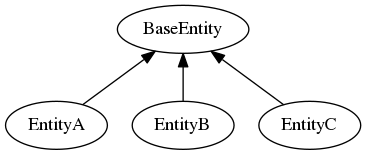
\includegraphics[width=0.65000\textwidth]{source/figures/generated/ecs/overview/oop/example_hierarchy_0.png}
\caption{Object-oriented inheritance: hypothetical entity hierarchy}
\end{figure}

\subsection{Implementation}\label{implementation}

This approach does not require any technique-specific implementation
detail. Since entity types have to conform to the same interface
\emph{(due to the use of run-time polymorphism)}, the \emph{``base
entity''} class is defined directly in the application's codebase. The
provided
\mintinline[numbersep=12pt, fontsize=\footnotesize, xleftmargin=17pt, linenos, mathescape, bgcolor=codebg]{text}{virtual}
interface greatly depends on the application itself. Some sort of
\emph{``manager''} class is usually defined as well, which keeps track
of the active entities and provides a convenient interface to perform
actions on them.

\subsubsection{Role-playing game}\label{role-playing-game-1}

To simulate the implementation of the example RPG, a hypothetical class
hierarchy is shown below:

\begin{figure}[htbp]
\centering
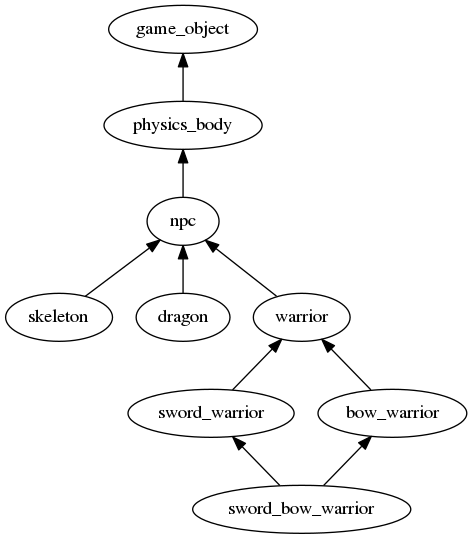
\includegraphics[width=0.70000\textwidth]{source/figures/generated/ecs/overview/oop/example_hierarchy_rpg.png}
\caption{Object-oriented inheritance: RPG entity hierarchy}
\end{figure}

The
\mintinline[numbersep=12pt, fontsize=\footnotesize, xleftmargin=17pt, linenos, mathescape, bgcolor=codebg]{text}{game_object}
entity type will be the base class from which all other game objects
derive - the interface has to be defined there:

\begin{minted}[numbersep=12pt, fontsize=\footnotesize, xleftmargin=17pt, linenos, mathescape]{cpp}
class game_object
{
public:
    virtual ~game_object() { }

    virtual void update(float dt) = 0;
    virtual void draw() = 0;
};
\end{minted}

The rest of the hierarchy is built upon
\mintinline[numbersep=12pt, fontsize=\footnotesize, xleftmargin=17pt, linenos, mathescape, bgcolor=codebg]{text}{game_object},
\textbf{incrementally} adding data and logic. Every game object that
follows the laws of physics will inherit from
\mintinline[numbersep=12pt, fontsize=\footnotesize, xleftmargin=17pt, linenos, mathescape, bgcolor=codebg]{text}{physics_body}:

\begin{minted}[numbersep=12pt, fontsize=\footnotesize, xleftmargin=17pt, linenos, mathescape]{cpp}
class physics_body : game_object
{
private:
    vector2f _position, _velocity;

public:
    void update(float dt) override
    {
        _position += _velocity * dt;
    }
};
\end{minted}

Physical objects that can be rendered and controlled by an AI will
inherit from
\mintinline[numbersep=12pt, fontsize=\footnotesize, xleftmargin=17pt, linenos, mathescape, bgcolor=codebg]{text}{npc}:

\begin{minted}[numbersep=12pt, fontsize=\footnotesize, xleftmargin=17pt, linenos, mathescape]{cpp}
class npc : physics_body
{
private:
    model* _model;
    texture* _texture;
    ai* _ai;

public:
    void update(float dt) override
    {
        physics_body::update(dt);
        _ai->think(dt);
    }

    void draw() override { /* ... */ }
};
\end{minted}

The leaves of the hierarchy tree will contain highly-specific data and
logic:

\begin{minted}[numbersep=12pt, fontsize=\footnotesize, xleftmargin=17pt, linenos, mathescape]{cpp}
class skeleton : npc { /* ... */ };
class dragon : npc { /* ... */ };
class warrior : npc { /* ... */ };

class sword_warrior : virtual warrior { /* ... */ };
class bow_warrior : virtual warrior { /* ... */ };

class sword_bow_warrior : sword_warrior, bow_warrior
{
    /* ... */
};
\end{minted}

To avoid code repetition during the implementation of a warrior that
simultaneously uses both a sword and a bow, a situation that requires
\emph{multiple inheritance} arises. A possible way of avoiding
duplicating the contents of the
\mintinline[numbersep=12pt, fontsize=\footnotesize, xleftmargin=17pt, linenos, mathescape, bgcolor=codebg]{text}{warrior}
class twice in
\mintinline[numbersep=12pt, fontsize=\footnotesize, xleftmargin=17pt, linenos, mathescape, bgcolor=codebg]{text}{sword_bow_warrior}
is using C++'s
\mintinline[numbersep=12pt, fontsize=\footnotesize, xleftmargin=17pt, linenos, mathescape, bgcolor=codebg]{text}{virtual}
inheritance feature, concisely explained in
{[}\protect\hyperlink{ref-cppreference_virtual_base_classes}{17}{]}.
These kind of hierarchies making use of multiple inheritance are
extremely cumbersome to maintain and expand: the pattern appearing in
\mintinline[numbersep=12pt, fontsize=\footnotesize, xleftmargin=17pt, linenos, mathescape, bgcolor=codebg]{text}{sword_bow_warrior}
is in fact commonly called \emph{``diamond of death''}.

\paragraph{\texorpdfstring{``Diamond of
death''}{Diamond of death}}\label{diamond-of-death}

The \textbf{``diamond of death''} \emph{(a.k.a. ``deadly diamond'' or
``common ancestor'' issue)} is a well-known problem that can appear in
object-oriented hierarchies. It was comprehensively covered in
{[}\protect\hyperlink{ref-truyen2004generalization}{18}{]}. An example
is found in this part of the previous hierarchy:

\begin{figure}[htbp]
\centering
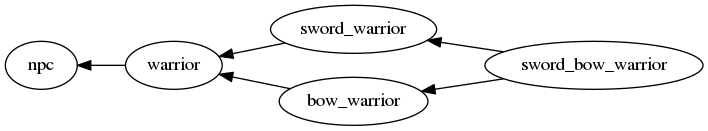
\includegraphics[width=0.85000\textwidth]{source/figures/generated/ecs/overview/oop/diamond_of_death.png}
\caption{OOP encoding issue: ``diamond of death''}
\end{figure}

The hierarchy causes \textbf{ambiguity} in case both
\mintinline[numbersep=12pt, fontsize=\footnotesize, xleftmargin=17pt, linenos, mathescape, bgcolor=codebg]{text}{sword_warrior}
and
\mintinline[numbersep=12pt, fontsize=\footnotesize, xleftmargin=17pt, linenos, mathescape, bgcolor=codebg]{text}{bow_warrior}
override the same method in
\mintinline[numbersep=12pt, fontsize=\footnotesize, xleftmargin=17pt, linenos, mathescape, bgcolor=codebg]{text}{warrior}
and causes \textbf{duplication} of
\mintinline[numbersep=12pt, fontsize=\footnotesize, xleftmargin=17pt, linenos, mathescape, bgcolor=codebg]{text}{warrior}'s
fields in
\mintinline[numbersep=12pt, fontsize=\footnotesize, xleftmargin=17pt, linenos, mathescape, bgcolor=codebg]{text}{sword_bow_warrior}.
To solve these problems, unless a feature like C++'s
\mintinline[numbersep=12pt, fontsize=\footnotesize, xleftmargin=17pt, linenos, mathescape, bgcolor=codebg]{text}{virtual}
inheritance is used, the class hierarchy has to be altered to avoid the
``diamond'', potentially introducing code repetition.

\subsubsection{GUI framework}\label{gui-framework-1}

An example implementation of the previously described imaginary GUI
framework will now be covered. As with the role-playing game, the proper
starting point is the class hierarchy. The base class of the framework
will be called
\mintinline[numbersep=12pt, fontsize=\footnotesize, xleftmargin=17pt, linenos, mathescape, bgcolor=codebg]{text}{widget}.
Unfortunately, the feature that allows widgets to be optionally animated
impedes the creation of a straightforward diagram and introduces the
\textbf{repetition problem}.

\paragraph{Repetition problem}\label{repetition-problem}

Handling optional animation features is problematic: a possible approach
would be defining a base
\mintinline[numbersep=12pt, fontsize=\footnotesize, xleftmargin=17pt, linenos, mathescape, bgcolor=codebg]{text}{animated_widget}
class and have all widgets derive from it.

\begin{figure}[htbp]
\centering
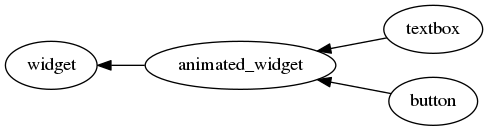
\includegraphics[width=0.75000\textwidth]{source/figures/generated/ecs/overview/oop/repetition_problem_0.png}
\caption{OOP encoding issue: repetition \#0}
\end{figure}

In the case shown above, all instances of
\mintinline[numbersep=12pt, fontsize=\footnotesize, xleftmargin=17pt, linenos, mathescape, bgcolor=codebg]{text}{textbox}
and
\mintinline[numbersep=12pt, fontsize=\footnotesize, xleftmargin=17pt, linenos, mathescape, bgcolor=codebg]{text}{button}
will have potentially unnecessary fields and methods if they do not make
use of the framework's animation capabilities. To solve this, one may
try to restructure the hierarchy as follows:

\begin{figure}[htbp]
\centering
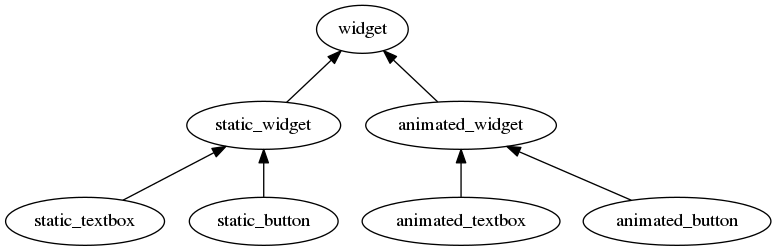
\includegraphics{source/figures/generated/ecs/overview/oop/repetition_problem_1.png}
\caption{OOP encoding issue: repetition \#1}
\end{figure}

Or in the following way:

\begin{figure}[htbp]
\centering
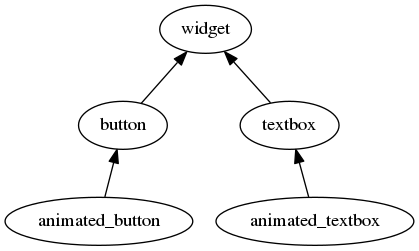
\includegraphics[width=0.70000\textwidth]{source/figures/generated/ecs/overview/oop/repetition_problem_2.png}
\caption{OOP encoding issue: repetition \#2}
\end{figure}

As the graphs show, \textbf{there is always some form of repetition in
one way or another}:

\begin{itemize}
\item
  In the first hierarchy, the widget data/logic for
  \mintinline[numbersep=12pt, fontsize=\footnotesize, xleftmargin=17pt, linenos, mathescape, bgcolor=codebg]{text}{textbox}
  and
  \mintinline[numbersep=12pt, fontsize=\footnotesize, xleftmargin=17pt, linenos, mathescape, bgcolor=codebg]{text}{button}
  has to be repeated for the
  \mintinline[numbersep=12pt, fontsize=\footnotesize, xleftmargin=17pt, linenos, mathescape, bgcolor=codebg]{text}{static_widget}
  and
  \mintinline[numbersep=12pt, fontsize=\footnotesize, xleftmargin=17pt, linenos, mathescape, bgcolor=codebg]{text}{animated_widget}
  branches of the hierarchies.
\item
  In the second hierarchy, the animation data/logic has to be repeated
  both for
  \mintinline[numbersep=12pt, fontsize=\footnotesize, xleftmargin=17pt, linenos, mathescape, bgcolor=codebg]{text}{textbox}
  and
  \mintinline[numbersep=12pt, fontsize=\footnotesize, xleftmargin=17pt, linenos, mathescape, bgcolor=codebg]{text}{button}.
\end{itemize}

Upon deciding between one of the hierarchies, the implementation does
not differ much from the RPG one: a
\mintinline[numbersep=12pt, fontsize=\footnotesize, xleftmargin=17pt, linenos, mathescape, bgcolor=codebg]{text}{widget}
base class will be created, with an interface all derived widgets must
conform to. The derived widget types will override
\mintinline[numbersep=12pt, fontsize=\footnotesize, xleftmargin=17pt, linenos, mathescape, bgcolor=codebg]{text}{widget}'s
methods to implement their logic.

\hypertarget{chapter_oop_communication}{\subsection{Communication}\label{chapter_oop_communication}}

Entity communication in this approach may need to occur for several
reasons, including:

\begin{itemize}
\item
  One entity needs to notify another entity about a particular event.

  \begin{itemize}
  \item
    \emph{Example:} the close button entity needs to inform the parent
    window that it needs to be closed.
  \item
    \emph{Example:} a ball hitting a brick in a Breakout clone needs to
    destroy the brick.
  \end{itemize}
\item
  An entity may be an aggregate of entities that need to cooperate.

  \begin{itemize}
  \tightlist
  \item
    \emph{Example:} a
    \mintinline[numbersep=12pt, fontsize=\footnotesize, xleftmargin=17pt, linenos, mathescape, bgcolor=codebg]{text}{tank}
    entity may be ``composed'' by a
    \mintinline[numbersep=12pt, fontsize=\footnotesize, xleftmargin=17pt, linenos, mathescape, bgcolor=codebg]{text}{cannon}
    entity and a
    \mintinline[numbersep=12pt, fontsize=\footnotesize, xleftmargin=17pt, linenos, mathescape, bgcolor=codebg]{text}{tracks}
    entity.
  \end{itemize}
\end{itemize}

\subsubsection{Address-based}\label{address-based}

Since entities are dynamically allocated, their location in memory does
not change during program execution. Senders that are \textbf{aware of
the lifetimes of their listeners} can effectively store pointers
\emph{(or references)} to them, in order to directly execute some of
their methods or mutate their
\mintinline[numbersep=12pt, fontsize=\footnotesize, xleftmargin=17pt, linenos, mathescape, bgcolor=codebg]{text}{public}
fields.

\begin{minted}[numbersep=12pt, fontsize=\footnotesize, xleftmargin=17pt, linenos, mathescape]{cpp}
class window : widget { /* ... */ };

class close_button : widget
{
private:
    window& _parent;

    // ...initialize fields on construction...

    void click()
    {
        _parent.close();
    }
};
\end{minted}

If senders are not aware of how long their receivers will live, or if
senders need to conditionally execute code depending on whether or not a
specific receiver is alive, this approach fails. Additional drawbacks
include harder networking and serialization, tightly coupled code which
is hard to reason about, and lack of flexibility. A possible alternative
given by the introduction of a \emph{mediator} class that deals with
entity creation and destruction, keeping track of entity states.

The mediator could generate \textbf{handles} that, similarly to
pointers, would allow access to entities' memory locations, but also add
an additional layer of indirection where the validity of the entity
pointed to by the handle can be checked.

\subsubsection{Subscription-based}\label{subscription-based}

Using a pattern similar to \textbf{``signals and slots''} or
\textbf{``events and delegates''}, it is possible to implement
inter-entity communication by subscribing/unsubscribing to events and
implementing event handlers. This approach solves the problem where the
sender is not aware of the lifetime of the receiver - the onus of
subscribing to specific event types lies on the receiver, that can
unsubscribe itself upon destruction.

The
\mintinline[numbersep=12pt, fontsize=\footnotesize, xleftmargin=17pt, linenos, mathescape, bgcolor=codebg]{text}{game_object}
class will contain an
\mintinline[numbersep=12pt, fontsize=\footnotesize, xleftmargin=17pt, linenos, mathescape, bgcolor=codebg]{text}{on_destruction}
event that will be invoked on entity destruction:

\begin{minted}[numbersep=12pt, fontsize=\footnotesize, xleftmargin=17pt, linenos, mathescape]{cpp}
class game_object
{
public:
    event on_destruction;
    // ...
};
\end{minted}

Game objects that need to communicate, like
\mintinline[numbersep=12pt, fontsize=\footnotesize, xleftmargin=17pt, linenos, mathescape, bgcolor=codebg]{text}{tank},
will provide subscribable events:

\begin{minted}[numbersep=12pt, fontsize=\footnotesize, xleftmargin=17pt, linenos, mathescape]{cpp}
class cannon : game_object { /* ... */ };
class tracks : game_object { /* ... */ };

class tank : game_object
{
public:
    event on_fire;
    // ...
};
\end{minted}

Entities will be \emph{``linked''} together after they have been
created:

\begin{minted}[numbersep=12pt, fontsize=\footnotesize, xleftmargin=17pt, linenos, mathescape]{cpp}
void link_tank_events(tank& tk, cannon& cn, tracks& ts)
{
    auto event_handle = tk.on_fire.subscribe([&]
        {
            ts.stop();
            cn.fire();
        });

    auto unsub_on_fire = [&tk, event_handle]
        {
            tk.on_fire.unsubscribe(event_handle);
        };

    cn.on_destruction(unsub_on_fire);
    ts.on_destruction(unsub_on_fire);
}
\end{minted}

While this approach provides some decoupling between entity types, it
also introduces unnecessary run-time overhead due to event management.
It is also unsafe, as application code needs to make sure entities with
subscribers outlive their subscribers \emph{(e.g.
\mintinline[numbersep=12pt, fontsize=\footnotesize, xleftmargin=17pt, linenos, mathescape, bgcolor=codebg]{text}{tk}
needs to outlive both
\mintinline[numbersep=12pt, fontsize=\footnotesize, xleftmargin=17pt, linenos, mathescape, bgcolor=codebg]{text}{cn}
and
\mintinline[numbersep=12pt, fontsize=\footnotesize, xleftmargin=17pt, linenos, mathescape, bgcolor=codebg]{text}{ts})}.

\subsubsection{Message-based}\label{message-based}

A superior technique, that decouples entity communication from the
entities themselves, consists in \textbf{producers} generating
\textbf{messages} that are forwarded to a \textbf{message queue} and
read by \textbf{consumers}. Message types can be implemented as a
\textbf{tagged}
\mintinline[numbersep=12pt, fontsize=\footnotesize, xleftmargin=17pt, linenos, mathescape, bgcolor=codebg]{text}{union}
of lightweight structs, by using run-time polymorphism, or by using a
variant type like
\mintinline[numbersep=12pt, fontsize=\footnotesize, xleftmargin=17pt, linenos, mathescape, bgcolor=codebg]{text}{boost::variant}:

\begin{minted}[numbersep=12pt, fontsize=\footnotesize, xleftmargin=17pt, linenos, mathescape]{cpp}
struct maximize_message { int _window_id; };
struct close_message { int _window_id; };

using message = variant<maximize_message, close_message>;
\end{minted}

After modeling the union of message types, the base entity class will
need to provide a
\mintinline[numbersep=12pt, fontsize=\footnotesize, xleftmargin=17pt, linenos, mathescape, bgcolor=codebg]{text}{virtual}
event handler method:

\begin{minted}[numbersep=12pt, fontsize=\footnotesize, xleftmargin=17pt, linenos, mathescape]{cpp}
class widget
{
protected:
    virtual handle_message(const message&) { }
    // ...
}
\end{minted}

Entities can create messages by enqueuing them in a shared
\mintinline[numbersep=12pt, fontsize=\footnotesize, xleftmargin=17pt, linenos, mathescape, bgcolor=codebg]{text}{message_queue}
object:

\begin{minted}[numbersep=12pt, fontsize=\footnotesize, xleftmargin=17pt, linenos, mathescape]{cpp}
class close_button : widget
{
private:
    int _parent_id;

    void click(message_queue& mq)
    {
        mq.enqueue(message{close_message{_parent_id}})
    }

    // ...
};
\end{minted}

Derived classes can override the event handler method to respond to
messages:

\begin{minted}[numbersep=12pt, fontsize=\footnotesize, xleftmargin=17pt, linenos, mathescape]{cpp}
class window : widget
{
private:
    int _id;

    void handle_message(const message& m) override
    {
        visit(m,
            [this](const maximize_message& x)
            {
                if(x._window_id == this->_id)
                    this->maximize();
            },
            [this](const close_message& x)
            {
                if(x._window_id == this->_id)
                    this->close();
            });
    }

    // ...
};
\end{minted}

This approach is versatile and can be implemented more cleverly and
efficiently, although it is rarely used outside of huge-scale projects
in practice. Entities never explicitly know about each other - they
``subscribe'' to particular message types instead and process them as
they arrive. When a sender or receiver entity is destroyed, it simply
stops sending or receiving messages, preventing erroneous memory
accesses.

\subsection{Advantages and
disadvantages}\label{advantages-and-disadvantages}

Compared to a completely \emph{unstructured} approach, using polymorphic
objects to encode entities provides a cleaner and simpler way of
managing data and logic. However, the object-oriented inheritance
technique is only suitable for simple applications and games with a
limited amount of entity types and a small number of active entity
instances at run-time. Its main selling point is the ease of development
and programming productivity.

The use of polymorphism negatively impacts performance and memory usage
in comparison to a data-oriented approach, especially because it makes
taking advantage of data locality and cache-friendliness
impossible\footnote{common reasons include: indirection and size
  overhead caused by dynamic allocation; loading unused fields in the
  cache. More information at
  {[}\protect\hyperlink{ref-ithare_allocations}{19}{]} and
  {[}\protect\hyperlink{ref-scee_oop_pitfalls}{20}{]}.}.

Using inheritance to build an entity type hierarchy lacks flexibility
and, as seen in the examples, introduces significant architectural
problems.

\section{Object-oriented composition}\label{object-oriented-composition}

A flexible way of solving the aforementioned \emph{repetition} and
\emph{diamond} issues requires a point-of-view shift from a hierarchical
approach to a \textbf{composition-based} one. Entities will be defined
as containers of small reusable \textbf{behaviors}\footnote{the term
  \textbf{``behavior''} is being used instead of \textbf{``component''}
  in order to clearly distinguish the two concepts, as the former
  contains and handles logic, in contrast to the latter.}, with the
following characteristics:

\begin{itemize}
\item
  Behaviors \textbf{store data} and \textbf{handle logic};
\item
  Behavior types \textbf{conform to the same interface} and
  polymorphically inherit from a base
  \mintinline[numbersep=12pt, fontsize=\footnotesize, xleftmargin=17pt, linenos, mathescape, bgcolor=codebg]{text}{behavior}
  class;
\item
  Behaviors can be added and removed from entities at run-time.
\end{itemize}

From a high-level perspective, object-oriented composition looks like
this:

\begin{figure}[htbp]
\centering
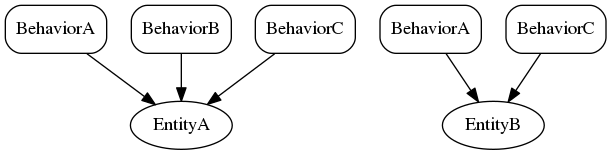
\includegraphics[width=0.75000\textwidth]{source/figures/generated/ecs/overview/oop_composition/example.png}
\caption{Object-oriented composition: hypotetical entity hierarchy}
\end{figure}

\subsection{Implementation}\label{implementation-1}

As with the previous approach, a base class containing an
application-specific
\mintinline[numbersep=12pt, fontsize=\footnotesize, xleftmargin=17pt, linenos, mathescape, bgcolor=codebg]{text}{virtual}
interface needs to be defined - this time the class will represent a
behavior type, not an entity type.

\subsubsection{Role-playing game}\label{role-playing-game-2}

Here is an example on how the
\mintinline[numbersep=12pt, fontsize=\footnotesize, xleftmargin=17pt, linenos, mathescape, bgcolor=codebg]{text}{skeleton}
and
\mintinline[numbersep=12pt, fontsize=\footnotesize, xleftmargin=17pt, linenos, mathescape, bgcolor=codebg]{text}{dragon}
entities could be encoded using object-oriented composition:

\begin{figure}[htbp]
\centering
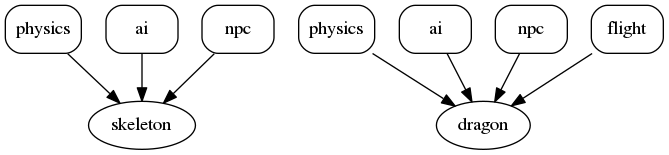
\includegraphics{source/figures/generated/ecs/overview/oop_composition/example_rpg_0.png}
\caption{Object-oriented composition: RPG - skeleton and dragon}
\end{figure}

This approach also solves the previously encountered ``diamond of
death'' issue:

\begin{figure}[htbp]
\centering
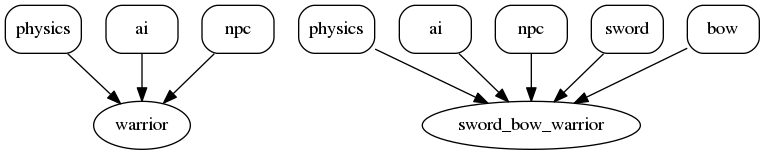
\includegraphics{source/figures/generated/ecs/overview/oop_composition/example_rpg_1.png}
\caption{Object-oriented composition: RPG - unarmed and sword+bow
warrior}
\end{figure}

The code for the base polymorphic
\mintinline[numbersep=12pt, fontsize=\footnotesize, xleftmargin=17pt, linenos, mathescape, bgcolor=codebg]{text}{behavior}
class closely resembles the previously seen
\mintinline[numbersep=12pt, fontsize=\footnotesize, xleftmargin=17pt, linenos, mathescape, bgcolor=codebg]{text}{game_object}:

\begin{minted}[numbersep=12pt, fontsize=\footnotesize, xleftmargin=17pt, linenos, mathescape]{cpp}
class behavior
{
public:
    virtual ~behavior() { }

    virtual void update(float dt) { }
    virtual void draw() { }
};


class physics : behavior { /* ... */ };
class ai : behavior { /* ... */ };
class npc : behavior { /* ... */ };
class flight : behavior { /* ... */ };
class sword : behavior { /* ... */ };
class bow : behavior { /* ... */ };
\end{minted}

The implementation of
\mintinline[numbersep=12pt, fontsize=\footnotesize, xleftmargin=17pt, linenos, mathescape, bgcolor=codebg]{text}{entity}
provides an interface to manipulate behaviors at run-time, and stores
the behaviors in a
\mintinline[numbersep=12pt, fontsize=\footnotesize, xleftmargin=17pt, linenos, mathescape, bgcolor=codebg]{text}{std::vector}
of
\mintinline[numbersep=12pt, fontsize=\footnotesize, xleftmargin=17pt, linenos, mathescape, bgcolor=codebg]{text}{std::unique_ptr<behavior>},
in order to enable polymorphism to correctly take place:

\begin{minted}[numbersep=12pt, fontsize=\footnotesize, xleftmargin=17pt, linenos, mathescape]{cpp}
class entity
{
private:
    std::vector<std::unique_ptr<behavior>> _behaviors;

public:
    template<typename T, typename... Ts>
    auto& emplace_behavior(Ts&&... xs) { /* ... */ }

    void update(float dt)
    {
        for(auto& c : _behaviors)
            c->update(dt);
    }

    void draw()
    {
        for(auto& c : _behaviors)
            c->draw();
    }
};
\end{minted}

Entity types \textbf{are not encoded as classes} anymore, but as
\textbf{functions} that return entity instances:

\begin{minted}[numbersep=12pt, fontsize=\footnotesize, xleftmargin=17pt, linenos, mathescape]{cpp}
auto make_skeleton(/* ... */)
{
    entity result;
    result.emplace_behavior<physics>(/* ... */);
    result.emplace_behavior<ai>(/* ... */);
    result.emplace_behavior<npc>(/* ... */);

    return result;
}
\end{minted}

\begin{minted}[numbersep=12pt, fontsize=\footnotesize, xleftmargin=17pt, linenos, mathescape]{cpp}
auto make_dragon(/* ... */)
{
    entity result;
    result.emplace_behavior<physics>(/* ... */);
    result.emplace_behavior<ai>(/* ... */);
    result.emplace_behavior<npc>(/* ... */);
    result.emplace_behavior<flight>(/* ... */);

    return result;
}
\end{minted}

\begin{minted}[numbersep=12pt, fontsize=\footnotesize, xleftmargin=17pt, linenos, mathescape]{cpp}
auto make_sword_bow_warrior(/* ... */)
{
    entity result;
    result.emplace_behavior<physics>(/* ... */);
    result.emplace_behavior<ai>(/* ... */);
    result.emplace_behavior<npc>(/* ... */);
    result.emplace_behavior<sword>(/* ... */);
    result.emplace_behavior<bow>(/* ... */);

    return result;
}
\end{minted}

\subsubsection{GUI framework}\label{gui-framework-2}

This technique solves the \textbf{repetition problem} encountered during
the object-oriented inheritance-based implementation of the example GUI
framework.

\begin{figure}[htbp]
\centering
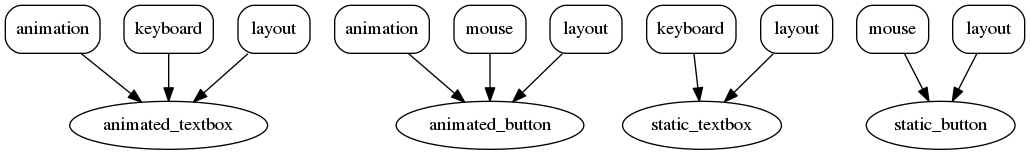
\includegraphics{source/figures/generated/ecs/overview/oop_composition/example_gui_0.png}
\caption{Object-oriented composition: GUI entity hierarchy}
\end{figure}

\subsection{Communication}\label{communication}

While entities still need to communicate with each other for the reasons
described in \protect\hyperlink{chapter_oop_communication}{Chapter 3,
Subsection 3.3.2}, this technique also may require that behaviors
``talk'' to one another.

Imagine implementing a
\mintinline[numbersep=12pt, fontsize=\footnotesize, xleftmargin=17pt, linenos, mathescape, bgcolor=codebg]{text}{clickable}
behavior for widgets:

\begin{minted}[numbersep=12pt, fontsize=\footnotesize, xleftmargin=17pt, linenos, mathescape]{cpp}
struct clickable : behavior
{
    bounding_box _bb;
    bool _clicked;

    void update(float) override
    {
        _clicked = mouse::overlaps(_bb);
    }
};
\end{minted}

Buttons and textboxes need to ``ask'' the
\mintinline[numbersep=12pt, fontsize=\footnotesize, xleftmargin=17pt, linenos, mathescape, bgcolor=codebg]{text}{clickable}
behavior whether or not they need to handle a mouse click.

\subsubsection{Address-based}\label{address-based-1}

A possible approach would be either checking or asserting the existence
of a behavior and then access it directly through the entity. A
requirement is that behaviors store a reference to their parent entity:

\begin{minted}[numbersep=12pt, fontsize=\footnotesize, xleftmargin=17pt, linenos, mathescape]{cpp}
class behavior
{
protected:
    entity& _entity;
    // ...
};

struct print_on_click : behavior
{
    void update(float) override
    {
        assert(_entity.has_behavior<clickable>());
        auto& bc = _entity.get_behavior<clickable>();

        if(bc._clicked) { /* ... */ }
    }
};
\end{minted}

This communication method quickly becomes hard to maintain due to heavy
coupling between behaviors.

\subsubsection{Message-based}\label{message-based-1}

Similarly to the object-oriented approach, using lightweight messages
and a mediator
\mintinline[numbersep=12pt, fontsize=\footnotesize, xleftmargin=17pt, linenos, mathescape, bgcolor=codebg]{text}{message_queue}
class can reduce coupling and make communication between behaviors much
easier to manage. The implementation is essentially equivalent to the
one previously shown: the base
\mintinline[numbersep=12pt, fontsize=\footnotesize, xleftmargin=17pt, linenos, mathescape, bgcolor=codebg]{text}{behavior}
type will provide a
\mintinline[numbersep=12pt, fontsize=\footnotesize, xleftmargin=17pt, linenos, mathescape, bgcolor=codebg]{text}{virtual handle_message(const message&)}
function that derived behavior types can override.

\subsection{Advantages and
disadvantages}\label{advantages-and-disadvantages-1}

Object-oriented composition is easy to implement and much more flexible
than the hierarchical approach, but it's still suboptimal compared to
data-oriented composition:

\begin{itemize}
\item
  No separation of data and logic is present;
\item
  There is a significant overhead due to run-time polymorphism;
\item
  It's still impossible to take advantage of the CPU cache.
\end{itemize}

A crucial piece of the ECS pattern, the \textbf{system}, is still
missing from this technique. Its introduction will allow a clean
separation of data and logic, that will lead to parallelization
opportunities and possible cache-friendliness. The introduction of the
system will allow to replace behaviors with logic-less
\textbf{components}.

\section{Data-oriented composition}\label{data-oriented-composition}

In order to make the most of a machine's hardware, a major development
paradigm shift has to be taken: enter \textbf{data-oriented design}. DOD
is \emph{all about the data}: code \textbf{has to be designed around the
data} and not vice-versa. When used correctly, data-oriented design can
allow applications to take advantage of parallelism and a higher
percentage of cache hits\footnote{cache-friendliness is obtained by
  storing data contiguously in memory, loading only necessary data in
  the cache, and avoiding indirection. See
  {[}\protect\hyperlink{ref-ithare_allocations}{19}{]} and
  {[}\protect\hyperlink{ref-scee_oop_pitfalls}{20}{]} for more details.}.
Additional benefits include modularity, easier networking, and easier
serialization.

To achieve all the aforementioned advantages, the following design will
be used:

\begin{itemize}
\item
  Entity instances will be simple \textbf{numerical IDs};
\item
  \textbf{Component types} will be simple, small and logic-less;
\item
  Component data will be \textbf{stored separately} from entities;
\item
  Logic will be separately handled by \textbf{systems};

  \begin{itemize}
  \tightlist
  \item
    Entities will subscribe to systems depending on their current active
    component types.
  \end{itemize}
\item
  A \textbf{context} \emph{(manager)} object will \textbf{tie everything
  together}.

  \begin{itemize}
  \tightlist
  \item
    The various parts of the pattern will communicate with each other
    and with the user through the context.
  \end{itemize}
\end{itemize}

An intuition for this technique is thinking about \textbf{relational
database management systems} \emph{(RDBMSs)} tables, with component
types as columns, and entity instances as rows:

\begin{longtable}[]{@{}lccc@{}}
\toprule
& ComponentA & ComponentB & ComponentC\tabularnewline
\midrule
\endhead
Entity \#0 & X & X &\tabularnewline
Entity \#1 & & X &\tabularnewline
Entity \#2 & X & & X\tabularnewline
\bottomrule
\end{longtable}

The table above shows how component types can be bound and unbound from
entity instances. The previously mentioned \textbf{context} object will
keep track of component availability in entity instances, thus providing
an interface roughly similar to
\mintinline[numbersep=12pt, fontsize=\footnotesize, xleftmargin=17pt, linenos, mathescape, bgcolor=codebg]{text}{bool context::has_component<...>(entity_id)}.

\begin{figure}[htbp]
\centering
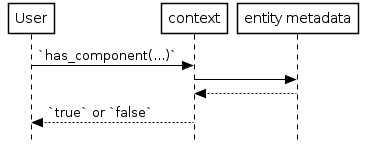
\includegraphics[width=0.65000\textwidth]{source/figures/generated/ecs/overview/dod_composition/uml_context_has_component.png}
\caption{DOD: checking component type availability through context
object}
\end{figure}

Knowing that an entity instance possesses a specific component type, a
function that retrieves the data of the component for that particular
instance will also be provided by the context object:
\mintinline[numbersep=12pt, fontsize=\footnotesize, xleftmargin=17pt, linenos, mathescape, bgcolor=codebg]{text}{auto& context::get_component<...>(entity_id)}.

\begin{figure}[htbp]
\centering
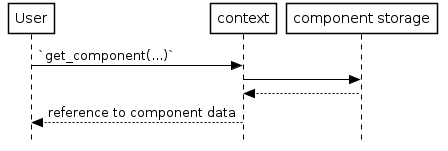
\includegraphics[width=0.65000\textwidth]{source/figures/generated/ecs/overview/dod_composition/uml_context_get_component.png}
\caption{DOD: getting component instance data through context object}
\end{figure}

The role of
\mintinline[numbersep=12pt, fontsize=\footnotesize, xleftmargin=17pt, linenos, mathescape, bgcolor=codebg]{text}{entity metadata}
and
\mintinline[numbersep=12pt, fontsize=\footnotesize, xleftmargin=17pt, linenos, mathescape, bgcolor=codebg]{text}{component storage}
in the diagrams is to show the additional layer of abstraction between
the user and the pattern implementation. With the introduction of the
\textbf{context object} concept, it is possible to cleanly implement
\textbf{systems}. They will ``ask'' the context to return the set of all
matching entities\footnote{in a real implementation, systems will
  efficiently cache the set of entities they match - the
  \mintinline[numbersep=12pt, fontsize=\footnotesize, xleftmargin=17pt, linenos, mathescape, bgcolor=codebg]{text}{context}
  will not have to continuously iterate over all existing entities.},
with an interface like
\mintinline[numbersep=12pt, fontsize=\footnotesize, xleftmargin=17pt, linenos, mathescape, bgcolor=codebg]{text}{void context::for_entities_with<...>(f)}.

\begin{figure}[htbp]
\centering
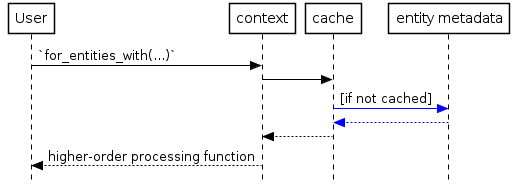
\includegraphics[width=0.75000\textwidth]{source/figures/generated/ecs/overview/dod_composition/uml_context_for_entities_with.png}
\caption{DOD: retrieving entities matching a component type set through
context object}
\end{figure}

Here is a user-code example system implementation:

\begin{minted}[numbersep=12pt, fontsize=\footnotesize, xleftmargin=17pt, linenos, mathescape]{cpp}
void example_system(context& c)
{
    c.for_entities_with<a_type, c_type>([&c](auto eid)
        {
            auto& a_data = c.get_component<a_type>(eid);
            auto& c_data = c.get_component<c_type>(eid);

            perform_action(a_data, c_data);
        });
}
\end{minted}

All the logic of the application can then be defined in terms of
sequential data transformations\footnote{``dataflow programming''.},
which are very easy to maintain, expand and parallelize. For instance,
\mintinline[numbersep=12pt, fontsize=\footnotesize, xleftmargin=17pt, linenos, mathescape, bgcolor=codebg]{text}{example_system}
could be parallelized by splitting the range provided by
\mintinline[numbersep=12pt, fontsize=\footnotesize, xleftmargin=17pt, linenos, mathescape, bgcolor=codebg]{text}{for_entities_with}
evenly between CPU cores.

The role of the context is to decouple entities, components and systems,
and provide a high level of abstraction. Component data could be stored
in \emph{arrays}, \emph{hash tables}, or even on another machine over
the network.

\begin{figure}[htbp]
\centering
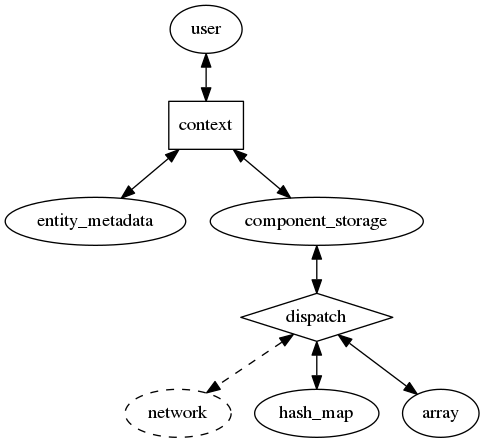
\includegraphics[width=0.75000\textwidth]{source/figures/generated/ecs/overview/dod_composition/context_role.png}
\caption{DOD: role of the context object}
\end{figure}

\subsection{Implementation}\label{implementation-2}

There are some implementation details inherently related to the
approach. Since entities are numerical IDs, it is sufficient to define a
type alias:

\begin{minted}[numbersep=12pt, fontsize=\footnotesize, xleftmargin=17pt, linenos, mathescape]{cpp}
using entity_id = std::size_t;
\end{minted}

If all component types and system types are supposed to be known at
compile-time, it is unnecessary to define base classes for them.
Implementing component storage can be done in multiple ways: the most
simple and straightforward way consists in using a separate array per
component type:

\begin{minted}[numbersep=12pt, fontsize=\footnotesize, xleftmargin=17pt, linenos, mathescape]{cpp}
struct component_a { /* ... */ };
struct component_b { /* ... */ };
struct component_c { /* ... */ };

constexpr auto max_entities{10000};

class component_storage
{
private:
    std::array<component_a, max_entities> _a;
    std::array<component_b, max_entities> _b;
    std::array<component_c, max_entities> _c;

public:
    template <typename TComponent>
    TComponent& get(entity_id eid);
};
\end{minted}

The
\mintinline[numbersep=12pt, fontsize=\footnotesize, xleftmargin=17pt, linenos, mathescape, bgcolor=codebg]{text}{context}
will take care of retrieving data from
\mintinline[numbersep=12pt, fontsize=\footnotesize, xleftmargin=17pt, linenos, mathescape, bgcolor=codebg]{text}{component_storage},
thus making the implementation of system types extremely simple:

\begin{minted}[numbersep=12pt, fontsize=\footnotesize, xleftmargin=17pt, linenos, mathescape]{cpp}
struct system_ac
{
    void process(context& c)
    {
        c.for_entities_with<a_type, c_type>([&c](auto eid)
            {
                 /* ... */
            });
    }
};
\end{minted}

The application code will roughly look like this:

\begin{minted}[numbersep=12pt, fontsize=\footnotesize, xleftmargin=17pt, linenos, mathescape]{cpp}
int main()
{
    component_storage cs;
    context c{cs};

    system_ac s_ac;

    // ...create entities...
    // ...add components...

    while(running)
    {
        s_ac.process(c);
    }
}
\end{minted}

All the leftover details can be implemented in multiple ways:

\begin{itemize}
\item
  Components can be bound to entities by using a \textbf{dense bitset},
  where every bit corresponds to a component type;

  \begin{itemize}
  \tightlist
  \item
    The bitsets and additional metadata can be stored in various ways -
    the
    \mintinline[numbersep=12pt, fontsize=\footnotesize, xleftmargin=17pt, linenos, mathescape, bgcolor=codebg]{text}{context}
    will take care of providing access to them.
  \end{itemize}
\item
  Systems can keep track of the subscribed entities by storing their IDs
  in an appropriate data structures;

  \begin{itemize}
  \tightlist
  \item
    The
    \mintinline[numbersep=12pt, fontsize=\footnotesize, xleftmargin=17pt, linenos, mathescape, bgcolor=codebg]{text}{context}
    can take care of matching entities to systems when a new entity is
    created or its components are changed.
  \end{itemize}
\item
  Components and entities can communicate with each other by allowing
  systems to produce outputs that can be processed by the application
  code.
\end{itemize}

\subsubsection{Role-playing game}\label{role-playing-game-3}

The class design is identical to the one seen in the object-oriented
composition approach. Instead of using
\mintinline[numbersep=12pt, fontsize=\footnotesize, xleftmargin=17pt, linenos, mathescape, bgcolor=codebg]{text}{behavior}
types that handle both data and logic, they are completely split: data
is stored in components, logic is handled by systems:

\begin{minted}[numbersep=12pt, fontsize=\footnotesize, xleftmargin=17pt, linenos, mathescape]{cpp}
// The namespace `c` will contain all component types.
namespace c
{
    struct physics { /* ... */ };
    struct ai { /* ... */ };
    struct npc { /* ... */ };
    struct flight { /* ... */ };
    struct sword { /* ... */ };
    struct bow { /* ... */ };
}

// The namespace `s` will contain all system types.
namespace s
{
    // Processes entities with `c::physics`.
    struct physics { /* ... */ };

    // Processes entities with `c::ai` and `c::npc`.
    struct ai_npc { /* ... */ };

    // ...
}
\end{minted}

Entity creation and mutation are delegated to the
\mintinline[numbersep=12pt, fontsize=\footnotesize, xleftmargin=17pt, linenos, mathescape, bgcolor=codebg]{text}{context},
which takes care of bookkeeping and binding all elements together:

\begin{minted}[numbersep=12pt, fontsize=\footnotesize, xleftmargin=17pt, linenos, mathescape]{cpp}
auto make_skeleton(context& c, /* ... */)
{
    auto eid = c.create_entity();
    c.emplace_component<physics>(eid, /* ... */);
    c.emplace_component<ai>(eid, /* ... */);
    c.emplace_component<npc>(eid, /* ... */);

    return eid;
}
\end{minted}

The application code or the
\mintinline[numbersep=12pt, fontsize=\footnotesize, xleftmargin=17pt, linenos, mathescape, bgcolor=codebg]{text}{context}
will take care of instantiating and executing systems. Systems that do
not depend on each other can be executed in parallel, and systems with
no processing ordering requirements can also be internally parallelized.

\subsubsection{GUI framework}\label{gui-framework-3}

The data-oriented implementation of the example GUI framework is
conceptually identically to the RPG one. A powerful benefit of using
systems to handle logic is that animation features are cleanly handled
and specialized for every widget type:

\begin{minted}[numbersep=12pt, fontsize=\footnotesize, xleftmargin=17pt, linenos, mathescape]{cpp}
namespace c
{
    struct animation { /* ... */ };
    struct layout { /* ... */ };
    struct keyboard { /* ... */ };
    struct mouse { /* ... */ };

    // Sometimes highly-specific components can be
    // defined to handle particular situations or to
    // simply "tag" entities.
    struct textbox { /* ... */ };
    struct button { /* ... */ };
}

namespace s
{
    // Processes entities with `c::textbox` and `c::keyboard`.
    struct textbox { /* ... */ };

    // Processes entities with `c::button` and `c::mouse`.
    struct button { /* ... */ };

    // Textbox-specific optional animations.
    // Processes entities with `c::textbox` and `c::animation`.
    struct anim_textbox { /* ... */ };

    // Button-specific optional animations.
    // Processes entities with `c::button` and `c::animation`.
    struct anim_button { /* ... */ };
}
\end{minted}

As seen from the above component and system definitions, the existence
of an
\mintinline[numbersep=12pt, fontsize=\footnotesize, xleftmargin=17pt, linenos, mathescape, bgcolor=codebg]{text}{animation}
component in an entity will either enable or disable optional
animations. If an entity has the
\mintinline[numbersep=12pt, fontsize=\footnotesize, xleftmargin=17pt, linenos, mathescape, bgcolor=codebg]{text}{animation}
component, the logic will depend on the other components the entity has,
making it easy to define widget-specific animation behavior.

All that is left is instantiating the
\mintinline[numbersep=12pt, fontsize=\footnotesize, xleftmargin=17pt, linenos, mathescape, bgcolor=codebg]{text}{context}
and the system types, then execute application-specific logic:

\begin{minted}[numbersep=12pt, fontsize=\footnotesize, xleftmargin=17pt, linenos, mathescape]{cpp}
int main()
{
    context c;

    s::textbox s_textbox;
    s::button s_button;
    s::anim_textbox s_anim_textbox;
    s::anim_button s_anim_button;

    // ...create entities and components...

    while(running)
    {
        s_textbox.process(c);
        s_button.process(c);
        s_anim_textbox.process(c);
        s_anim_button.process(c);
    }
}
\end{minted}

The boilerplate code shown in the code snippet above can be avoided by
using advanced metaprogramming techniques. In
\protect\hyperlink{part2_ecst}{Part 2}, the way \textbf{ECST} avoids
similar bookkeeping code will be analyzed.

\subsection{Communication}\label{communication-1}

\subsubsection{Inter-component}\label{inter-component}

Systems elegantly solve the problem of inter-component communication.
Imagine a simple physics simulation using the following components:

\begin{minted}[numbersep=12pt, fontsize=\footnotesize, xleftmargin=17pt, linenos, mathescape]{cpp}
struct position { vec3f _v };
struct velocity { vec3f _v };
struct acceleration { vec3f _v };
\end{minted}

Two systems can be used to implement \(v' = v + a\) and \(p' = p + v\),
allowing
\mintinline[numbersep=12pt, fontsize=\footnotesize, xleftmargin=17pt, linenos, mathescape, bgcolor=codebg]{text}{velocity}
to communicate with
\mintinline[numbersep=12pt, fontsize=\footnotesize, xleftmargin=17pt, linenos, mathescape, bgcolor=codebg]{text}{acceleration}
and
\mintinline[numbersep=12pt, fontsize=\footnotesize, xleftmargin=17pt, linenos, mathescape, bgcolor=codebg]{text}{position}
to communicate with
\mintinline[numbersep=12pt, fontsize=\footnotesize, xleftmargin=17pt, linenos, mathescape, bgcolor=codebg]{text}{velocity}:

\begin{minted}[numbersep=12pt, fontsize=\footnotesize, xleftmargin=17pt, linenos, mathescape]{cpp}
void process_acceleration(context& c)
{
    c.for_entities_with<velocity, acceleration>([&c](auto eid)
        {
            c.get_component<velocity>(eid)._v +=
                c.get_component<acceleration>(eid)._v;
        });
}

void process_velocity(context& c)
{
    c.for_entities_with<position, velocity>([&c](auto eid)
        {
            c.get_component<position>(eid)._v +=
                c.get_component<velocity>(eid)._v;
        });
};
\end{minted}

\hypertarget{sys_streamqueue}{\subsubsection{Inter-system}\label{sys_streamqueue}}

Inter-system communication can also be very useful. Consider situations
where multiple system dependency chains run in parallel: some systems
may require forwarding information to the next system in the chain.

There are various ways of solving this problem:

\begin{itemize}
\item
  Systems could be stateful \emph{(storing their outputs, so that others
  can access them)} and could store references to other systems.
  Particular care must be used in making sure that a system has finished
  processing before accessing its output and that its memory location
  does not change.

  \begin{figure}[htbp]
  \centering
  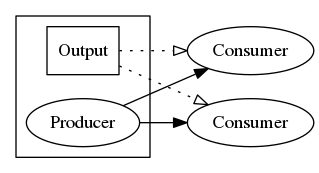
\includegraphics[width=0.55000\textwidth]{source/figures/generated/ecs/overview/dod_composition/output_system_communication.png}
  \caption{DOD communication: example stateful system communication
  architecture}
  \end{figure}
\item
  A \textbf{streaming} technique using queues could be used in certain
  situations \emph{(depending on the implementation of the systems)} -
  one system would act as a \emph{producer} and other systems would act
  as \emph{consumers}. The producer system would enqueue messages during
  entity processing - other systems would not directly process entities,
  instead process received messages.

  \begin{figure}[htbp]
  \centering
  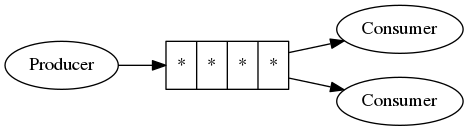
\includegraphics[width=0.70000\textwidth]{source/figures/generated/ecs/overview/dod_composition/queue_system_communication.png}
  \caption{DOD communication: example streaming system communication
  architecture}
  \end{figure}
\end{itemize}

\subsubsection{Inter-entity}\label{inter-entity}

Inter-entity communication is not as useful as in the previous encoding
techniques, but some particular situations may require specific entity
instances to share data. \emph{``Inter-entity''} is a misnomer, as
logic-less entities cannot directly communicate together - specialized
systems will have to initiate and resolve inter-entity messages. This
can be achieved in multiple ways:

\begin{itemize}
\item
  Systems can produce special outputs containing the IDs of the entities
  that intend to communicate and a particular message. Subsequent
  systems will take care of processing those outputs and performing
  actions depending on the type/contents of the messages.
\item
  A thread-safe queue can be accessed by systems during execution to
  enqueue messages. Subsequent systems can sequentially dequeue all
  messages and directly act upon entity instances depending on the
  type/contents of the messages.
\end{itemize}

Having two tightly coupled entity instances when using the
Entity-Component-System pattern is a red flag: it is very likely that
the coupling can be avoided by introducing new components and/or
systems, or by modifying the design of the application.

\subsection{Advantages and
disadvantages}\label{advantages-and-disadvantages-2}

Using data-oriented composition, all the benefits of object-oriented
composition are maintained, but several new advantages are achieved:

\begin{itemize}
\item
  Data and logic \textbf{are separated};
\item
  The code becomes \textbf{more modular}, easier to maintain and extend;
\item
  Entities are more easily \textbf{serializable}\footnote{the use of
    numerical IDs instead of pointers and the separation of data and
    logic make serialization trivial.} and \textbf{synchronizable} over
  the network;
\item
  Entities can be processed in terms of \textbf{chained data
  transformations}, allowing parallelization and cache-friendliness;
\item
  No unnecessary run-time polymorphism overhead.
\end{itemize}

One \emph{perceived} disadvantage may be that the code is harder to
reason about compared to an object-oriented approach, and inherently
less abstracted. One of the objectives of this thesis is showing that,
with a proper ECS library, the code is \textbf{actually easier to reason
about} \emph{(thanks to a dataflow-oriented approach)} and that
high-level abstractions \emph{(and the safety/convenience they provide)}
do \textbf{not have to be sacrificed}.

In addition, data-oriented composition lends itself very nicely to
multi-machine parallel computing - a real-world example is Improbable's
\textbf{SpatialOS} cloud-based architecture
{[}\protect\hyperlink{ref-spatialos_learnmore}{21}{]}, which massively
parallelizes computation in a transparent way using a variant of the
Entity-Component-System pattern.

\section{Conclusion}\label{conclusion}

A gradual transition from a traditional \textbf{object-oriented
inheritance} entity encoding technique to a \textbf{data-oriented
composition} one was shown in this chapter. The data-oriented
composition approach allows an efficient and correct implementation of
the \textbf{Entity-Component-System} pattern.

Every analyzed entity encoding technique has several advantages and
drawbacks - the complexity of a project is the most important parameter
to consider when choosing between them.

\part{ECST}

\hypertarget{part2_ecst}{\chapter{Overview}\label{part2_ecst}}

\textbf{ECST} is a \textbf{C++14} library designed to let users
implement the \textbf{Entity-Component-System} pattern in their
applications leveraging \textbf{compile-time} knowledge of component
types, data-structures and system dependencies to allow
\textbf{automatic parallelization} of separate data transformation
chains.

The source code is available on GitHub under the \emph{Academic Free
License (``AFL'') v. 3.0}: \url{https://github.com/SuperV1234/ecst}.

\section{Design}\label{design}

The library was designed to allow users to safely implement the ECS
pattern using an \textbf{high-level of abstraction} without sacrificing
\textbf{performance} and \textbf{flexibility}, using knowledge of the
supported component and system types at compile-time.

\subsection{Compile-time ECS}\label{compile-time-ecs}

Every feature offered by ECST requires the instantiation of a
\textbf{context} template class \emph{(whose role is the management of
the entire pattern)} which provides the user with a high-level interface
to interact with entities, components and systems. The context object
requires \textbf{prior knowledge} of all \textbf{component types} and
\textbf{system types} at compile-time. Additionally, options regarding
multithreading support, system scheduling and entity limits can be
specified before the instantiation of a context.

Due to these factors, ECST is \textbf{not a data-driven}
Entity-Component-System library. If the target application domain
requires dynamic run-time composition and flexibility, it is sensible
\emph{(and recommended)} to use ECST with an additional data-driven ECS
library\footnote{ECST can be used to implement engine-level components
  and systems, while an additional data-driven library provides run-time
  flexibility and extensibility. Integration with ECST could be achieved
  by creating a ``bridge'' component that links entities between the two
  libraries.}.

\begin{itemize}
\item
  All component and system types must be known at compile-time;
\item
  Entities can be created, destroyed, tracked and mutated at run-time.
\end{itemize}

Some disadvantages of this approach include:

\begin{itemize}
\item
  Longer and potentially-unreadable errors;
\item
  Increased compilation times.
\end{itemize}

The implementation details regarding the definition and usage of
compile-time settings will be explored in
\protect\hyperlink{chap_ecst_metaprogramming}{Chapter 6} and
\protect\hyperlink{chap_ecst_compilemtime}{Chapter 7}. To make the
following points simpler to understand and to give the readers an idea
of the previously mentioned limitations and features, the code snippet
below will illustrate how context objects are configured and
instantiated in the user code.

\hypertarget{code_example_settings_definition}{\subsubsection{Code
example: settings definition}\label{code_example_settings_definition}}

Imagine a 2D particle simulation composed by:

\begin{itemize}
\item
  Three component types: \textbf{Position}, \textbf{Velocity}, and
  \textbf{Acceleration}.
\item
  Two system types: \textbf{Velocity} and \textbf{Acceleration}.
\end{itemize}

Component types are defined as simple \textbf{POD}
\emph{(plain-old-data)}
\mintinline[numbersep=12pt, fontsize=\footnotesize, xleftmargin=17pt, linenos, mathescape, bgcolor=codebg]{text}{struct}
types.

\begin{minted}[numbersep=12pt, fontsize=\footnotesize, xleftmargin=17pt, linenos, mathescape]{cpp}
// The namespace `c` will contain all component types.
namespace c
{
    struct position { /* ... */ };
    struct velocity { /* ... */ };
    struct acceleration { /* ... */ };
}
\end{minted}

System types are declared as
\mintinline[numbersep=12pt, fontsize=\footnotesize, xleftmargin=17pt, linenos, mathescape, bgcolor=codebg]{text}{struct}
types that will eventually be defined alongside their processing logic.

\begin{minted}[numbersep=12pt, fontsize=\footnotesize, xleftmargin=17pt, linenos, mathescape]{cpp}
//The namespace `s` will contain all system types.
namespace s
{
    struct velocity;
    struct acceleration;
}
\end{minted}

ECST makes heavy use of the \textbf{type-value-encoding} \emph{(a.k.a.
dependent typing)} meta-programming paradigm. It is necessary to define
wrapper
\mintinline[numbersep=12pt, fontsize=\footnotesize, xleftmargin=17pt, linenos, mathescape, bgcolor=codebg]{text}{constexpr}
\textbf{tag} values that will store the type information of components
and systems: tags are be used to greatly simplify both the user
interface \emph{(as accessing template methods in C++ requires the
cumbersome
\mintinline[numbersep=12pt, fontsize=\footnotesize, xleftmargin=17pt, linenos, mathescape, bgcolor=codebg]{text}{.template}
disambiguation syntax)} and implementation code.

Component tags are defined using
\mintinline[numbersep=12pt, fontsize=\footnotesize, xleftmargin=17pt, linenos, mathescape, bgcolor=codebg]{text}{ecst::tag::component::v}:

\begin{minted}[numbersep=12pt, fontsize=\footnotesize, xleftmargin=17pt, linenos, mathescape]{cpp}
// The namespace `ct` will contain all component tags.
namespace ct
{
    constexpr auto position =
        ecst::tag::component::v<c::position>;

    constexpr auto velocity =
        ecst::tag::component::v<c::velocity>;

    constexpr auto acceleration =
        ecst::tag::component::v<c::acceleration>;
}
\end{minted}

System tags are defined using
\mintinline[numbersep=12pt, fontsize=\footnotesize, xleftmargin=17pt, linenos, mathescape, bgcolor=codebg]{text}{ecst::tag::system::v}:

\begin{minted}[numbersep=12pt, fontsize=\footnotesize, xleftmargin=17pt, linenos, mathescape]{cpp}
// The namespace `st` will contain all system tags.
namespace st
{
    constexpr auto velocity =
        ecst::tag::system::v<c::velocity>;

    constexpr auto acceleration =
        ecst::tag::system::v<c::acceleration>;
}
\end{minted}

The verbosity of the code shown above can be avoided through the use of
convenient preprocessor macros. The definition of tag objects only needs
to occur once in the entire user codebase.

Having defined all required types and tags, the next step will consist
in defining \emph{signatures}:

\begin{itemize}
\item
  \textbf{Component signatures} bind component tags to \textbf{storage
  policies}.
\item
  \textbf{System signatures} bind system tags to multiple settings which
  will be analyzed in depth in \protect\hyperlink{system_sigs}{Chapter
  7, Subsection 7.1.2}: \textbf{parallelization policies} and
  \textbf{dependencies} can be found among them.
\end{itemize}

Signatures are stored in compile-time type lists called
\textbf{signature lists}, which must be forwarded to the context
creation, in order to instantiate a context object.

The
\mintinline[numbersep=12pt, fontsize=\footnotesize, xleftmargin=17pt, linenos, mathescape, bgcolor=codebg]{text}{make_csl()}
function will create a component signature for every previously-defined
component tag, and will return a component signature list holding all of
them.

\begin{minted}[numbersep=12pt, fontsize=\footnotesize, xleftmargin=17pt, linenos, mathescape]{cpp}
constexpr auto make_csl()
{
    // Component signature namespace aliases.
    namespace sc = ecst::signature::component;
    namespace slc = ecst::signature_list::component;

    // Store `c::acceleration`, `c::velocity` and `c::position` in
    // three separate contiguous buffers (SoA).
    constexpr auto cs_acceleration =
        sc::make(ct::acceleration).contiguous_buffer();

    constexpr auto cs_velocity =
        sc::make(ct::velocity).contiguous_buffer();

    constexpr auto cs_position =
        sc::make(ct::position).contiguous_buffer();

    // Build and return the "component signature list".
    return slc::make(cs_acceleration, cs_velocity, cs_position);
}
\end{minted}

The
\mintinline[numbersep=12pt, fontsize=\footnotesize, xleftmargin=17pt, linenos, mathescape, bgcolor=codebg]{text}{make_ssl()}
function will create a system signature for every previously-defined
system tag, and will return a system signature list holding all of them.

\begin{minted}[numbersep=12pt, fontsize=\footnotesize, xleftmargin=17pt, linenos, mathescape]{cpp}
constexpr auto make_ssl()
{
    // System signature namespace aliases.
    namespace ss = ecst::signature::system;
    namespace sls = ecst::signature_list::system;

    // Acceleration system signature.
    constexpr auto ss_acceleration =
        ss::make(st::acceleration)
            .parallelism(split_evenly_per_core)
            .read(ct::acceleration)
            .write(ct::velocity);

    // Velocity system signature.
    constexpr auto ss_velocity =
        ss::make(st::velocity)
            .dependencies(st::acceleration)
            .parallelism(split_evenly_per_core)
            .read(ct::velocity)
            .write(ct::position);

    // Build and return the "system signature list".
    return sls::make(ss_acceleration, ss_velocity);
}
\end{minted}

The final setup step consists in the definition of a
\mintinline[numbersep=12pt, fontsize=\footnotesize, xleftmargin=17pt, linenos, mathescape, bgcolor=codebg]{text}{constexpr}
\textbf{context settings} instance, which will be used to instantiate an
ECST context.

\begin{minted}[numbersep=12pt, fontsize=\footnotesize, xleftmargin=17pt, linenos, mathescape]{cpp}
constexpr auto context_settings =
    ecst::settings::make()
        .component_signatures(make_csl())
        .system_signatures(make_ssl())

auto context =
    ecst::context::make(context_settings);
\end{minted}

Note that this example skipped many possible configuration options and
implementation and design details for the current settings definition
approach: the goal of the code snippets above is to clarify that
component and system types \emph{need} to be known at compile-time and
\emph{how} that information is passed to an ECST context. The knowledge
provided by
\mintinline[numbersep=12pt, fontsize=\footnotesize, xleftmargin=17pt, linenos, mathescape, bgcolor=codebg]{text}{context_settings}
will be used to \textbf{generate} the following elements at
\textbf{compile-time}:

\begin{itemize}
\item
  Storage for \protect\hyperlink{storage_entity}{\textbf{entity
  metadata}}, \protect\hyperlink{storage_component}{\textbf{component
  data}}, and \protect\hyperlink{storage_system}{\textbf{systems}};
\item
  An implicit \textbf{system dependency graph}, which is used to
  automatically run different systems in parallel.
\end{itemize}

Easily interchangeable compile-time options also allow developers to
experiment with different data layouts and scheduling policies without
having to modify the application code.

\subsection{Customizability}\label{customizability}

The compile-time-driven nature of the library lends itself to
\textbf{policy-based design} for user-configurable options. In line with
the \emph{``pay for what you use''} C++ philosophy, the specified
policies are taken into account in various ways to optimize run-time
performance and memory usage.

All featured options will be analyzed in
\protect\hyperlink{chap_ecst_compiletime}{Chapter 7}. As a simple
example, the following code snippet that generates two different context
instances can help understand the power of policy-based settings:

\subsubsection{Code example: policy-based
customization}\label{code-example-policy-based-customization}

\begin{minted}[numbersep=12pt, fontsize=\footnotesize, xleftmargin=17pt, linenos, mathescape]{cpp}
constexpr auto context_settings_0 =
    ecst::settings::make()
        .allow_inner_parallelism()
        .fixed_entity_limit(ecst::sz_v<10000>);

constexpr auto context_settings_1 =
    ecst::settings::make()
        .disallow_inner_parallelism()
        .dynamic_entity_limit()
        .scheduler(cs::scheduler<user_defined_scheduler>);
\end{minted}

Note how easy and intuitive it is to change major library components and
affect the flexibility and performance of user applications. This
pattern is not only used in context settings definition, but also in
component and system signatures \emph{(e.g.~inner parallelism policies
or system dependencies)}.

The approach also favours \textbf{test-driven-development} and
application code \textbf{transparency}: tests and benchmarks covering
various combinations of policies \emph{(either exhaustively or with a
fuzzy approach)} can be easily generated by using nested compile-time
loops over desired policy lists, thus providing information regarding
the correctness and performance of the user code.

\subsection{Abstraction, user-friendliness, and
safety}\label{abstraction-user-friendliness-and-safety}

A common misconception regarding \textbf{data-oriented design} is that
it's necessary to sacrifice \textbf{encapsulation} and to \textbf{reduce
the level of abstraction} in order to achieve performance and
cache-friendliness. The following beliefs are commonly found in online
discussions:

\begin{itemize}
\item
  High-level multi-paradigm languages like \textbf{C++14} or \textbf{D}
  are not suitable for high-performance DOD because they inherently
  drive programmers to design highly-abstracted code that is not closely
  mapped to the machine hardware. The origin of this belief can be
  attributed to the abuse of OOP techniques, such as run-time
  polymorphism and encapsulation, which tend to increase the level of
  abstraction, with the side-effect of harming data locality and leading
  to suboptimal memory layouts;
\item
  Every abstraction has an intrinsic cost \emph{(``there is no such
  thing as cost-free abstractions'')}.
\end{itemize}

These misbeliefs may result in the fallacy that performant DOD code must
be devoid of high-level abstractions.

ECST aims to \emph{counter this fallacy} by providing a high-level
interface that does not sacrifice run-time performance thanks to C++14
\textbf{cost-free abstractions}. Benefits of a highly-abstracted
data-oriented ECS library include:

\begin{itemize}
\item
  \textbf{User-friendly} and \textbf{transparent} syntax. No explicit
  storage or pointer management is required, and application code is
  independent of user-defined settings and policies;
\item
  Higher \textbf{safety}, as many development mistakes regarding
  dependencies and data access can be caught at compile-time;
\item
  Easier \textbf{testability}, due to the fact that abstracting settings
  and policies allows tests to run comprehensively over a wide set of
  option combinations;

  \begin{itemize}
  \tightlist
  \item
    Closely related, the possibility of quickly \textbf{experimenting}
    with different strategies is also a major benefit of a higher
    abstraction level.
  \end{itemize}
\item
  \textbf{Encapsulation}, \textbf{reusability}, and fulfillment of the
  \textbf{DRY} principle: abstracting and templatizing storage
  strategies and policies allows code to be conveniently reused.
\end{itemize}

\subsubsection{Syntax-level
transparency}\label{ecstoverview_syntaxtransp}

One important design goal of ECST is allowing the user to experiment
with different policies, schedulers and execution methods
\textbf{without having to explicitly change the application code}. This
objective is achieved through the use of \textbf{proxy} objects and
heavily-templatized type-value-encoding implementation code. The result
is a \textbf{syntax-level transparency} that allows the application code
to be completely independent of compile-time policies/strategies.

Proxies and transparency implementation details will be covered in
\protect\hyperlink{chap_proxies}{Chapter 11} - a simple code example
will illustrate one possible use of syntax-level transparency through
proxies.

\subsubsection{Code example: transparency through
proxies}\label{code-example-transparency-through-proxies}

Here's a possible implementation of the
\mintinline[numbersep=12pt, fontsize=\footnotesize, xleftmargin=17pt, linenos, mathescape, bgcolor=codebg]{text}{s::velocity}
system declared in
\protect\hyperlink{code_example_settings_definition}{Subsection 4.1.1}:

\begin{minted}[numbersep=12pt, fontsize=\footnotesize, xleftmargin=17pt, linenos, mathescape]{cpp}
struct velocity
{
    template<typename TData>
    void process(TData& data)
    {
        data.for_entities([](auto eid)
        {
            auto& position =
                data.get(ct::position, eid)._v;

            const auto& velocity =
                data.get(ct::velocity, eid)._v;

            position += velocity;
        });
    }
};
\end{minted}

The
\mintinline[numbersep=12pt, fontsize=\footnotesize, xleftmargin=17pt, linenos, mathescape, bgcolor=codebg]{text}{velocity}
system
\mintinline[numbersep=12pt, fontsize=\footnotesize, xleftmargin=17pt, linenos, mathescape, bgcolor=codebg]{text}{struct}
contains a
\mintinline[numbersep=12pt, fontsize=\footnotesize, xleftmargin=17pt, linenos, mathescape, bgcolor=codebg]{text}{process}
template method that takes a single
\mintinline[numbersep=12pt, fontsize=\footnotesize, xleftmargin=17pt, linenos, mathescape, bgcolor=codebg]{text}{TData& data}
\emph{lvalue reference} as its argument \emph{(note that
\mintinline[numbersep=12pt, fontsize=\footnotesize, xleftmargin=17pt, linenos, mathescape, bgcolor=codebg]{text}{process}
is not a special method that is specifically recognized by ECST)}.
\mintinline[numbersep=12pt, fontsize=\footnotesize, xleftmargin=17pt, linenos, mathescape, bgcolor=codebg]{text}{data}
is a \textbf{data proxy} object, which abstracts the operations of a
system behind a \textbf{safe and transparent} interface.

By invoking the
\mintinline[numbersep=12pt, fontsize=\footnotesize, xleftmargin=17pt, linenos, mathescape, bgcolor=codebg]{text}{data.for_entities}
method with a callable object, it is possible to iterate over the
entities subscribed to the system, and perform some actions on the
component they own. In this case, we're accessing the
\mintinline[numbersep=12pt, fontsize=\footnotesize, xleftmargin=17pt, linenos, mathescape, bgcolor=codebg]{text}{c::position}
component through a mutable reference, and the
\mintinline[numbersep=12pt, fontsize=\footnotesize, xleftmargin=17pt, linenos, mathescape, bgcolor=codebg]{text}{c::velocity}
component through a
\mintinline[numbersep=12pt, fontsize=\footnotesize, xleftmargin=17pt, linenos, mathescape, bgcolor=codebg]{text}{const}
reference, in order to move the particle by its velocity.

The interesting thing is that this syntax is \textbf{completely
independent} of the system settings and execution policies - the
system's dependencies or parallelism policies do not matter to the data
proxy. Other things to take notice of are:

\begin{itemize}
\item
  The storage policy of the components is irrelevant.
  \mintinline[numbersep=12pt, fontsize=\footnotesize, xleftmargin=17pt, linenos, mathescape, bgcolor=codebg]{text}{c::position}
  and
  \mintinline[numbersep=12pt, fontsize=\footnotesize, xleftmargin=17pt, linenos, mathescape, bgcolor=codebg]{text}{c::velocity}
  could be stored in the same contiguous buffer, or one of them could be
  in an hash-map while the other one is in a machine on the other side
  of the world \emph{(storing a component in a different continent could
  slightly affect the performance of your application)};
\item
  Getting a mutable or
  \mintinline[numbersep=12pt, fontsize=\footnotesize, xleftmargin=17pt, linenos, mathescape, bgcolor=codebg]{text}{const}
  reference to a component is \textbf{statically checked} at
  compile-time, producing an error in case the component access does not
  fulfill what was specified in the system signature;
\item
  \mintinline[numbersep=12pt, fontsize=\footnotesize, xleftmargin=17pt, linenos, mathescape, bgcolor=codebg]{text}{process}
  is not special, and not limited to a single argument - additional data
  could be passed to the method and captured in the lambda. This will be
  covered in detail in \protect\hyperlink{chap_flow}{Chapter 8} - here's
  a possible way of invoking
  \mintinline[numbersep=12pt, fontsize=\footnotesize, xleftmargin=17pt, linenos, mathescape, bgcolor=codebg]{text}{s::velocity::process}:

  \begin{minted}[numbersep=12pt, fontsize=\footnotesize, xleftmargin=17pt, linenos, mathescape]{cpp}
  namespace sea = ecst::system_execution_adapter;

  context.step([](auto& proxy)
  {
      proxy.execute_systems(
          sea::t(st::velocity).for_subtasks(
              [](auto& s, auto& data)
              {
                  s.process(data);
              })
      );
  });
  \end{minted}
\end{itemize}

\subsection{Multithreading model}\label{multithreading-model}

The library was designed with user-friendly multithreading as one of the
primary goals, which is achieved by providing two levels of parallelism
that considerably increase application performance in the presence of
multiple CPU cores: \textbf{``outer parallelism''} and \textbf{``inner
parallelism''}.

Multithreading support is enabled by default, but can be switched off
completely or only in particular systems.

\hypertarget{overview_outer_parallelism_dag}{\subsubsection{Outer
parallelism}\label{overview_outer_parallelism_dag}}

\textbf{``Outer parallelism''} is the term used in ECST which defines
the concept of running multiple systems that do not depend on each other
in parallel. Its implementation details will be analyzed in
\protect\hyperlink{multithreading_system_scheduling}{Chapter 10}.
Conceptually, an \textbf{implicit directed acyclic graph} is created at
compile-time thanks to the knowledge of system dependencies. The
execution of the implicit DAG is handled by a \textbf{system scheduler}
type specified during settings definition.

Consider the previously defined system signatures - an implicit DAG
isomorphic to the one below will be generated by ECST \emph{(arrows
between nodes should be read as ``depends on'')}:

\begin{figure}[htbp]
\centering
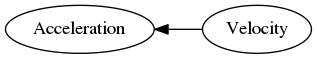
\includegraphics[width=0.50000\textwidth]{source/figures/generated/ecst/overview/multithreading/outer/dag0.png}
\caption{ECST multithreading: example outer parallelism DAG \#0}
\end{figure}

The graph makes it obvious that no outer parallelism can take place
here. Increasing the number of component and system types introduces
separate dependency chains - imagine the addition of \textbf{Growth},
\textbf{Shape}, \textbf{Rotation} and \textbf{Rendering} systems for a
graphical particle simulation:

\begin{figure}[htbp]
\centering
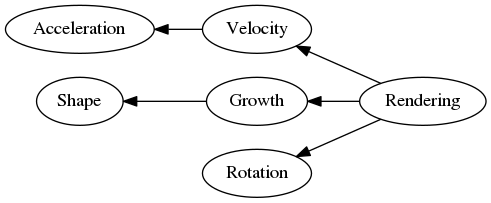
\includegraphics[width=0.65000\textwidth]{source/figures/generated/ecst/overview/multithreading/outer/dag1.png}
\caption{ECST multithreading: example outer parallelism DAG \#1}
\end{figure}

The DAG now shows three separate dependency chains:

\begin{itemize}
\item
  Rendering → Velocity → Acceleration;
\item
  Rendering → Growth → Shape;
\item
  Rendering → Rotation.
\end{itemize}

The chains starting with \textbf{Acceleration}, \textbf{Shape} and
\textbf{Rotation} can be executed in parallel. The \textbf{Rendering}
system will wait until all three chains have been successfully executed,
then it will process its subscribed entities.

Note that the user does not have to specify these chains anywhere - they
are implicitly created thanks to the dependencies described during
system signature definition.

\subsubsection{Inner parallelism}\label{inner-parallelism}

Other that running separate systems in parallel, ECST supports splitting
a single system into multiple \textbf{sub-tasks}, which can be executed
on separate threads. Many systems, such as the ones that represent
functionally pure computations, do not contain \emph{side-effects} that
modify their own state or that define interactions between the
subscribed entities: these are prime examples of
\textbf{``embarrassingly parallel''} computations. In contrast, some
systems \emph{(e.g.~broad-phase collision spatial partitioning)} require
processing their subscribed entities on a single thread, in order to
update data structures without explicit locking mechanisms\footnote{some
  systems need to mutate a data structure during execution. Splitting
  them in separate subtasks requires \emph{explicit locking} or a
  \emph{thread-safe} data structure to avoid race conditions. It is
  often more efficient to simply run these systems in a single subtask.}.

The aforementioned \textbf{Velocity} and \textbf{Acceleration} systems
are suited for inner parallelism. The user can enable inner parallelism
when defining system signatures, also choosing an \textbf{inner
parallelism strategy} that can be generated by composing multiple
strategies together \emph{(e.g. ``split into 4 sub-tasks only if
subscribed entity count is more than 100000'')}.

Imagine applying a \emph{``split into 4 sub-tasks''} strategy to
\textbf{Velocity} and \textbf{Acceleration} - the resulting DAG would
look as follows:

\begin{figure}[htbp]
\centering
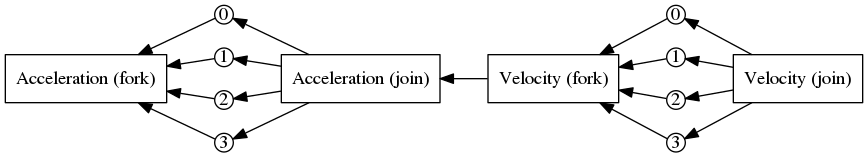
\includegraphics{source/figures/generated/ecst/overview/multithreading/inner/dag0.png}
\caption{ECST multithreading: example inner parallelism DAG}
\end{figure}

This allows the \(0..4\) sub-tasks to run in parallel. Commonly,
\textbf{inner parallelism executors}, which implement inner parallelism
policies, simply split the subscribed entities of a system evenly
between the generated subtasks. The \emph{``fork''} and \emph{``join''}
nodes present in the DAG are implicit - they can however be handled by
users thanks to \textbf{system execution adapters} \emph{(described in
\protect\hyperlink{chap_advfeats}{the ``advanced features'' chapter})},
allowing to code execution before and/or after the execution of a
system's sub-tasks.

\chapter{Architecture}\label{architecture}

Before analyzing the code and techniques used to implement ECST, the
architecture of the library will be examined.

A very high-level view of ECST's architecture can be illustrated as
such:

\begin{figure}[htbp]
\centering
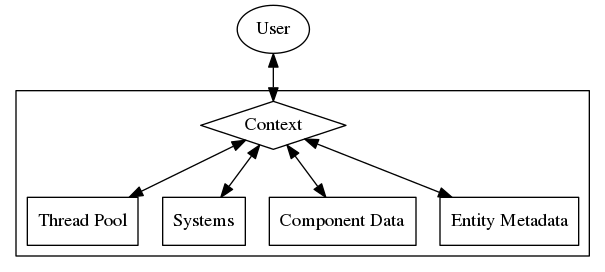
\includegraphics[width=0.75000\textwidth]{source/figures/generated/ecst/architecture/high_level.png}
\caption{ECST architecture: high-level overview}
\end{figure}

By looking at the diagram, it is obvious that the roles of the context
are:

\begin{itemize}
\item
  Providing a \textbf{friendly interface} between the user and the
  library;
\item
  \textbf{Decoupling} entities, components, and systems.
\end{itemize}

\section{Context}\label{context}

In the current version of the library, the
\mintinline[numbersep=12pt, fontsize=\footnotesize, xleftmargin=17pt, linenos, mathescape, bgcolor=codebg]{text}{context}
stores entity, system and component data.

\begin{itemize}
\item
  The composition of the \textbf{entity metadata storage} and of the
  \textbf{component data storage} is called
  \mintinline[numbersep=12pt, fontsize=\footnotesize, xleftmargin=17pt, linenos, mathescape, bgcolor=codebg]{text}{main_storage}.
\item
  The element managing systems, threads, and scheduling is called the
  \mintinline[numbersep=12pt, fontsize=\footnotesize, xleftmargin=17pt, linenos, mathescape, bgcolor=codebg]{text}{system_manager}.
\end{itemize}

\begin{figure}[htbp]
\centering
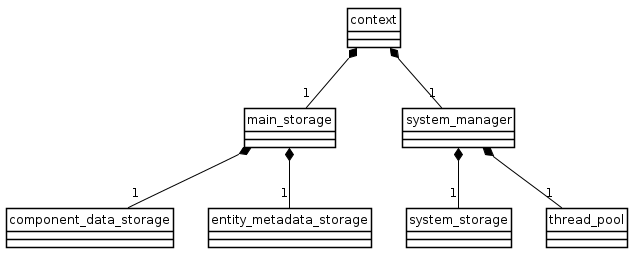
\includegraphics[width=0.80000\textwidth]{source/figures/generated/ecst/architecture/context_aggregation.png}
\caption{ECST architecture: context}
\end{figure}

\subsection{Entity metadata storage}\label{entity-metadata-storage}

The \textbf{entity metadata storage} contains
\mintinline[numbersep=12pt, fontsize=\footnotesize, xleftmargin=17pt, linenos, mathescape, bgcolor=codebg]{text}{metadata}
instances for every entity, which are used to:

\begin{itemize}
\item
  Keep track of the component types an entity possesses;
\item
  Map entities to handles and check their validity.
\end{itemize}

It also manages unused and used entity IDs.

\begin{figure}[htbp]
\centering
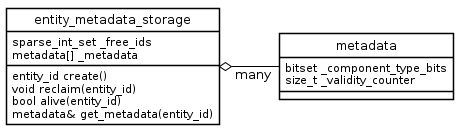
\includegraphics[width=0.75000\textwidth]{source/figures/generated/ecst/architecture/entity_metadata_storage.png}
\caption{ECST architecture: entity metadata storage}
\end{figure}

\subsection{Component data storage}\label{component-data-storage}

The \textbf{component data storage} contains
\mintinline[numbersep=12pt, fontsize=\footnotesize, xleftmargin=17pt, linenos, mathescape, bgcolor=codebg]{text}{chunk}
instances for every component signature type. \textbf{Chunks} store the
data of one or more component types with a user-specified strategy
\emph{(e.g.~contiguous buffer or hash map)} and provide a way to
retrieve references to component data given entity IDs.

\begin{figure}[htbp]
\centering
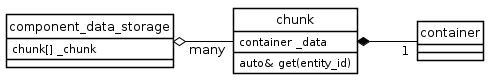
\includegraphics[width=0.85000\textwidth]{source/figures/generated/ecst/architecture/component_data_storage.png}
\caption{ECST architecture: component data storage}
\end{figure}

\hypertarget{architecture_system_mgr}{\subsection{System
manager}\label{architecture_system_mgr}}

The system manager contains:

\begin{itemize}
\item
  A
  \mintinline[numbersep=12pt, fontsize=\footnotesize, xleftmargin=17pt, linenos, mathescape, bgcolor=codebg]{text}{thread_pool}
  instance, used to efficiently execute system logic in separate
  threads;
\item
  A
  \mintinline[numbersep=12pt, fontsize=\footnotesize, xleftmargin=17pt, linenos, mathescape, bgcolor=codebg]{text}{system_storage},
  which stores an
  \mintinline[numbersep=12pt, fontsize=\footnotesize, xleftmargin=17pt, linenos, mathescape, bgcolor=codebg]{text}{instance}
  for every system signature type.

  \begin{itemize}
  \tightlist
  \item
    \textbf{Instances} store an instance of the user-provided system
    type and system metadata.
  \end{itemize}
\end{itemize}

\begin{figure}[htbp]
\centering
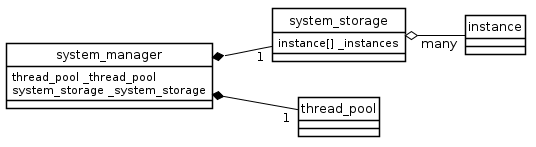
\includegraphics[width=0.85000\textwidth]{source/figures/generated/ecst/architecture/system_manager.png}
\caption{ECST architecture: system manager}
\end{figure}

\subsubsection{Instances}\label{instances}

Instances wrap user-provided systems, storing an instance of the
``real'' system type and additional metadata:

\begin{itemize}
\item
  A
  \mintinline[numbersep=12pt, fontsize=\footnotesize, xleftmargin=17pt, linenos, mathescape, bgcolor=codebg]{text}{state_manager},
  containing
  \mintinline[numbersep=12pt, fontsize=\footnotesize, xleftmargin=17pt, linenos, mathescape, bgcolor=codebg]{text}{state}
  instances;

  \begin{itemize}
  \tightlist
  \item
    Every subtask executed by an
    \mintinline[numbersep=12pt, fontsize=\footnotesize, xleftmargin=17pt, linenos, mathescape, bgcolor=codebg]{text}{instance}
    has its own
    \mintinline[numbersep=12pt, fontsize=\footnotesize, xleftmargin=17pt, linenos, mathescape, bgcolor=codebg]{text}{state},
    which contains eventual \emph{system output}, \emph{deferred
    functions}\footnote{used to delay the execution of functions in a
      later synchronous step.}, and IDs of entities to reclaim.
  \end{itemize}
\item
  A \emph{sparse integer set}\footnote{``sparse integer sets'' are very
    efficient data structures for the management of entity IDs. They are
    covered in \protect\hyperlink{appendix_sparse_integer_sets}{Chapter
    14, Section 14.1}.} tracking the entity IDs subscribed to the
  instance;
\item
  A \emph{dense bitset}\footnote{\mintinline[numbersep=12pt, fontsize=\footnotesize, xleftmargin=17pt, linenos, mathescape, bgcolor=codebg]{text}{std::bitset}.}
  representing the set of component types required for system
  subscription.
\end{itemize}

\begin{figure}[htbp]
\centering
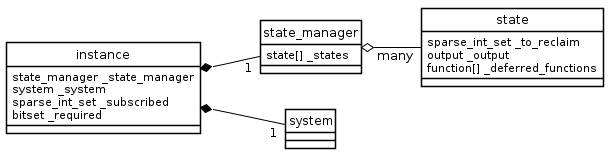
\includegraphics{source/figures/generated/ecst/architecture/instance.png}
\caption{ECST architecture: system instance}
\end{figure}

\hypertarget{chap_ecst_metaprogramming}{\chapter{Metaprogramming}\label{chap_ecst_metaprogramming}}

Before diving into Entity-Component-System related implementation
details, the \textbf{metaprogramming} techniques used throughout the
library will be covered in this chapter, as understanding them is a
prerequisite for the analysis of ECST's modules.

\section{Boost.Hana}\label{boost.hana}

\textbf{Boost.Hana} {[}\protect\hyperlink{ref-boosthana}{22}{]} is an
astonishing modern \emph{header-only} C++14 metaprogramming library
created \href{http://ldionne.com/}{by Louis Dionne} that uses the
\textbf{type-value encoding} paradigm \emph{(a.k.a. dependent typing
{[}\protect\hyperlink{ref-pfultz2_dependentyping}{23}{]})} - it is
heavily used throughout ECST's implementation. By wrapping types in
values, Hana allows users to perform both type-level computations and
heterogeneous computations using natural syntax\footnote{syntax that
  ``looks like'' regular run-time computation syntax.} and with minimal
compilation time overhead.

A simple example, taken from the original documentation, shows the idea
behind type-value encoding:

\begin{minted}[numbersep=12pt, fontsize=\footnotesize, xleftmargin=17pt, linenos, mathescape]{cpp}
auto animal_types = hana::make_tuple(
    hana::type_c<Fish*>, hana::type_c<Cat&>, hana::type_c<Dog>);

auto no_pointers = hana::remove_if(animal_types, [](auto a) {
    return hana::traits::is_pointer(a);
});

static_assert(no_pointers ==
    hana::make_tuple(hana::type_c<Cat&>, hana::type_c<Dog>), "");
\end{minted}

As seen in the code snippet above, types can be manipulated as values
\emph{(even using lambdas)}. Hana provides a huge number of powerful
algorithms and utilities that work both on types and ``traditional''
values.

As an example, component and system signature lists are implemented as
\href{http://www.boost.org/doc/libs/1_61_0/libs/hana/doc/html/structboost_1_1hana_1_1basic__tuple.html}{\mintinline[numbersep=12pt, fontsize=\footnotesize, xleftmargin=17pt, linenos, mathescape, bgcolor=codebg]{text}{boost::hana::basic_tuple}}
instances containing the user-specified signature types wrapped in
\href{http://www.boost.org/doc/libs/1_61_0/libs/hana/doc/html/structboost_1_1hana_1_1type.html\#ae35139e732c4b75e91061513cf445628}{\mintinline[numbersep=12pt, fontsize=\footnotesize, xleftmargin=17pt, linenos, mathescape, bgcolor=codebg]{text}{boost::hana::type_c}}
instances, which can be passed around like any other value and easily
manipulated.

\hypertarget{metaprogramming_tags}{\section{Tags}\label{metaprogramming_tags}}

\subsection{Motivation and usage}\label{motivation-and-usage}

A very large number of methods in the library is parametrized on
component types and system types. User code calling those methods would
normally require the constant and inelegant use of the
\mintinline[numbersep=12pt, fontsize=\footnotesize, xleftmargin=17pt, linenos, mathescape, bgcolor=codebg]{text}{instance.template method<...>(...)}
template disambiguation syntax\footnote{such syntax negatively impacts
  the readability of the code and is essentially avoidable boilerplate.
  It is required due to ambiguous parsing for the
  \mintinline[numbersep=12pt, fontsize=\footnotesize, xleftmargin=17pt, linenos, mathescape, bgcolor=codebg]{text}{<}
  token, which could be interpreted both as an \emph{``angle bracket''}
  or as a \emph{less-than operator}. Details can be found
  \href{http://en.cppreference.com/w/cpp/language/dependent_name\#The_template_disambiguator_for_dependent_names}{on
  cppreference}.}. \textbf{Tags} are designed to solve this problem.

Examples will be used in order to easily explain the role of tags. Here
is an hypotetical set of component and system types:

\begin{minted}[numbersep=12pt, fontsize=\footnotesize, xleftmargin=17pt, linenos, mathescape]{cpp}
namespace c
{
    struct position { /* ... */ };
    struct velocity { /* ... */ };
    struct acceleration { /* ... */ };
}

namespace s
{
    struct velocity { /* ... */ };
    struct acceleration { /* ... */ };
}
\end{minted}

Imagine a function that creates a particle using the components listed
above using ``traditional'' template method calling syntax:

\begin{minted}[numbersep=12pt, fontsize=\footnotesize, xleftmargin=17pt, linenos, mathescape]{cpp}
auto make_particle = [](auto& proxy)
{
    auto eid = proxy.create_entity();

    proxy.template add_component<c::position>(eid);
    proxy.template add_component<c::velocity>(eid);
    proxy.template add_component<c::acceleration>(eid);

    return eid;
};
\end{minted}

In order to prevent the mandatory
\mintinline[numbersep=12pt, fontsize=\footnotesize, xleftmargin=17pt, linenos, mathescape, bgcolor=codebg]{text}{.template}
disambiguation syntax and to treat component and system types as values,
ECST provides \textbf{component tags} and \textbf{system tags}.
\textbf{Tags} are
\mintinline[numbersep=12pt, fontsize=\footnotesize, xleftmargin=17pt, linenos, mathescape, bgcolor=codebg]{text}{constexpr}
wrappers that store the type information of components and systems in
values, allowing them to be conveniently passed to implementation and
interface functions with a natural syntax.

Tags need to be defined by the user, with the following syntax\footnote{preprocessor
  macros can be used to reduce required boilerplate code.}.

\begin{minted}[numbersep=12pt, fontsize=\footnotesize, xleftmargin=17pt, linenos, mathescape]{cpp}
// The namespace `ct` will contain all component tags.
namespace ct
{
    constexpr auto position =
        ecst::tag::component::v<c::position>;

    constexpr auto velocity =
        ecst::tag::component::v<c::velocity>;

    constexpr auto acceleration =
        ecst::tag::component::v<c::acceleration>;
}
\end{minted}

It is a good practice to separate \emph{component types}, \emph{system
types}, \emph{component tags} and \emph{system tags} in separate
namespaces.

\begin{minted}[numbersep=12pt, fontsize=\footnotesize, xleftmargin=17pt, linenos, mathescape]{cpp}
// The namespace `st` will contain all system tags.
namespace st
{
    constexpr auto velocity =
        ecst::tag::system::v<c::velocity>;

    constexpr auto acceleration =
        ecst::tag::system::v<c::acceleration>;
}
\end{minted}

Afterwards, calling template methods becomes much more natural:

\begin{minted}[numbersep=12pt, fontsize=\footnotesize, xleftmargin=17pt, linenos, mathescape]{cpp}
auto make_particle = [](auto& proxy)
{
    auto eid = proxy.create_entity();

    proxy.add_component(ct::position, eid);
    proxy.add_component(ct::velocity, eid);
    proxy.add_component(ct::acceleration, eid);

    return eid;
};
\end{minted}

Manipulating and storing tags is also easier, both in user and
implementation code, resulting in a more maintainable and extensible
codebase.

\subsection{Implementation}\label{implementation-3}

All tag-related types and functions are declared in the
\mintinline[numbersep=12pt, fontsize=\footnotesize, xleftmargin=17pt, linenos, mathescape, bgcolor=codebg]{text}{ecst::tag}
namespace. Both component tags and system tags are implemented in the
same way: a
\mintinline[numbersep=12pt, fontsize=\footnotesize, xleftmargin=17pt, linenos, mathescape, bgcolor=codebg]{text}{struct}
deriving from
\href{http://www.boost.org/doc/libs/1_61_0/libs/hana/doc/html/structboost_1_1hana_1_1type.html}{\mintinline[numbersep=12pt, fontsize=\footnotesize, xleftmargin=17pt, linenos, mathescape, bgcolor=codebg]{text}{boost::hana::type}}
is defined, that can be immediately used in any Boost.Hana algorithm.

\begin{minted}[numbersep=12pt, fontsize=\footnotesize, xleftmargin=17pt, linenos, mathescape]{cpp}
namespace impl
{
    template <typename T>
    struct tag_impl : public boost::hana::type<T> { };
}
\end{minted}

A
\mintinline[numbersep=12pt, fontsize=\footnotesize, xleftmargin=17pt, linenos, mathescape, bgcolor=codebg]{text}{constexpr}
variable called
\mintinline[numbersep=12pt, fontsize=\footnotesize, xleftmargin=17pt, linenos, mathescape, bgcolor=codebg]{text}{v}
\emph{(standing for ``value'')} is provided as a convenient way for the
user to define tags:

\begin{minted}[numbersep=12pt, fontsize=\footnotesize, xleftmargin=17pt, linenos, mathescape]{cpp}
template <typename T>
constexpr auto v = impl::tag_impl<T>{};
\end{minted}

The types encoded inside tags can be accessed using
\mintinline[numbersep=12pt, fontsize=\footnotesize, xleftmargin=17pt, linenos, mathescape, bgcolor=codebg]{text}{ecst::mp::unwrap}\footnote{the
  \mintinline[numbersep=12pt, fontsize=\footnotesize, xleftmargin=17pt, linenos, mathescape, bgcolor=codebg]{text}{ecst::mp}
  namespace contains metaprogramming-related utilities.}, which is a
type alias for types stored inside
\href{http://www.boost.org/doc/libs/1_61_0/libs/hana/doc/html/structboost_1_1hana_1_1type.html}{\mintinline[numbersep=12pt, fontsize=\footnotesize, xleftmargin=17pt, linenos, mathescape, bgcolor=codebg]{text}{boost::hana::type}}:

\begin{minted}[numbersep=12pt, fontsize=\footnotesize, xleftmargin=17pt, linenos, mathescape]{cpp}
namespace mp
{
    template <typename T>
    using unwrap = typename T::type;
}
\end{minted}

Converting a traditional template method to a tag-accepting one is a
straightforward process: the original method is hidden using the
\mintinline[numbersep=12pt, fontsize=\footnotesize, xleftmargin=17pt, linenos, mathescape, bgcolor=codebg]{text}{private}
access specifier - the new one will call it by \emph{unwrapping} the
tag:

\begin{minted}[numbersep=12pt, fontsize=\footnotesize, xleftmargin=17pt, linenos, mathescape]{cpp}
struct example
{
private:
    template <typename TComponent>
    auto& access_component(entity_id);

public:
    template <typename TComponentTag>
    auto& access_component(TComponentTag, entity_id eid)
    {
        return access_component<mp::unwrap<TComponentTag>>(eid);
    }
};
\end{minted}

Checking if a type or a value is a tag is also possible thanks to the
following utilities:

\begin{minted}[numbersep=12pt, fontsize=\footnotesize, xleftmargin=17pt, linenos, mathescape]{cpp}
namespace impl
{
    template <typename T>
    constexpr auto is_tag_impl =
        mp::is_specialization_of_v<tag_impl, T>;

    struct valid_t
    {
        template <typename... Ts>
        constexpr auto operator()(Ts...) const
        {
            return mp::list::all_variadic(is_tag_impl<Ts>...);
        }
    };
}

// Evaluates to true if all `xs...` are component tags.
constexpr impl::valid_t valid{};
\end{minted}

Note that
\mintinline[numbersep=12pt, fontsize=\footnotesize, xleftmargin=17pt, linenos, mathescape, bgcolor=codebg]{text}{valid}
is implemented as a
\mintinline[numbersep=12pt, fontsize=\footnotesize, xleftmargin=17pt, linenos, mathescape, bgcolor=codebg]{text}{constexpr}
value \emph{(instance of
\mintinline[numbersep=12pt, fontsize=\footnotesize, xleftmargin=17pt, linenos, mathescape, bgcolor=codebg]{text}{impl::valid_t})}
and not as a regular function. This pattern is used throughout ECST, due
to the fact that functions implemented as
\mintinline[numbersep=12pt, fontsize=\footnotesize, xleftmargin=17pt, linenos, mathescape, bgcolor=codebg]{text}{constexpr}
instances of callable objects can be easily used as arguments to other
functions without the need of a lambda wrapper. This is the case for the
\mintinline[numbersep=12pt, fontsize=\footnotesize, xleftmargin=17pt, linenos, mathescape, bgcolor=codebg]{text}{tag::component::is_list}
and
\mintinline[numbersep=12pt, fontsize=\footnotesize, xleftmargin=17pt, linenos, mathescape, bgcolor=codebg]{text}{tag::system::is_list}
functions, that return whether or not the passed argument is a list of
tags:

\begin{minted}[numbersep=12pt, fontsize=\footnotesize, xleftmargin=17pt, linenos, mathescape]{cpp}
template <typename T>
constexpr auto is_list(T x)
{
    return boost::hana::all_of(x, valid);
}
\end{minted}

\hypertarget{metaprogramming_option_maps}{\section{Option
maps}\label{metaprogramming_option_maps}}

\subsection{Motivation and usage}\label{motivation-and-usage-1}

User-provided compile-time settings are a vital part of ECST: in order
to allow users to set options in a convenient and clear way,
\textbf{option maps} were implemented using
\href{http://www.boost.org/doc/libs/1_61_0/libs/hana/doc/html/structboost_1_1hana_1_1map.html}{\mintinline[numbersep=12pt, fontsize=\footnotesize, xleftmargin=17pt, linenos, mathescape, bgcolor=codebg]{text}{boost::hana::map}}
instances and method chaining. Here is an example of user code that
creates a \emph{system signature} for
\mintinline[numbersep=12pt, fontsize=\footnotesize, xleftmargin=17pt, linenos, mathescape, bgcolor=codebg]{text}{s::acceleration}:

\begin{minted}[numbersep=12pt, fontsize=\footnotesize, xleftmargin=17pt, linenos, mathescape]{cpp}
constexpr auto ss_acceleration =
    ss::make(st::acceleration)
        .parallelism(split_evenly_per_core)
        .read(ct::acceleration)
        .write(ct::velocity);
\end{minted}

The code snippet above defines
\mintinline[numbersep=12pt, fontsize=\footnotesize, xleftmargin=17pt, linenos, mathescape, bgcolor=codebg]{text}{ss_acceleration}
to be a system signature for
\mintinline[numbersep=12pt, fontsize=\footnotesize, xleftmargin=17pt, linenos, mathescape, bgcolor=codebg]{text}{s::acceleration}
with the following settings, known at \textbf{compile-time}:

\begin{itemize}
\item
  Use the
  \mintinline[numbersep=12pt, fontsize=\footnotesize, xleftmargin=17pt, linenos, mathescape, bgcolor=codebg]{text}{split_evenly_per_core}
  \emph{inner parallelism strategy};
\item
  Use the
  \mintinline[numbersep=12pt, fontsize=\footnotesize, xleftmargin=17pt, linenos, mathescape, bgcolor=codebg]{text}{c::acceleration}
  component (read-only);
\item
  Use the
  \mintinline[numbersep=12pt, fontsize=\footnotesize, xleftmargin=17pt, linenos, mathescape, bgcolor=codebg]{text}{c::velocity}
  component (mutable).
\end{itemize}

The options are provided by the user by chaining methods such as
\mintinline[numbersep=12pt, fontsize=\footnotesize, xleftmargin=17pt, linenos, mathescape, bgcolor=codebg]{text}{.parallelism(...)}
and
\mintinline[numbersep=12pt, fontsize=\footnotesize, xleftmargin=17pt, linenos, mathescape, bgcolor=codebg]{text}{.read(...)}.
The calls can be freely re-ordered, and if the same method is
accidentally called twice, a compile-time error will be generated.

Defining settings using the pattern above is possible thanks to the
\mintinline[numbersep=12pt, fontsize=\footnotesize, xleftmargin=17pt, linenos, mathescape, bgcolor=codebg]{text}{ecst::mp::option_map}
compile-time data structure.

\subsection{Implementation}\label{implementation-4}

Conceptually, an option map is a compile-time associative container with
the following properties:

\begin{itemize}
\item
  Keys are values fulfilling the Boost.Hana
  \href{http://www.boost.org/doc/libs/1_61_0/libs/hana/doc/html/group__group-Comparable.html}{\mintinline[numbersep=12pt, fontsize=\footnotesize, xleftmargin=17pt, linenos, mathescape, bgcolor=codebg]{text}{Comparable}}
  and
  \href{http://www.boost.org/doc/libs/1_61_0/libs/hana/doc/html/group__group-Hashable.html}{\mintinline[numbersep=12pt, fontsize=\footnotesize, xleftmargin=17pt, linenos, mathescape, bgcolor=codebg]{text}{Hashable}}
  concept;

  \begin{itemize}
  \tightlist
  \item
    A set of keys is composed by
    \mintinline[numbersep=12pt, fontsize=\footnotesize, xleftmargin=17pt, linenos, mathescape, bgcolor=codebg]{text}{constexpr}
    \href{http://www.boost.org/doc/libs/1_61_0/libs/hana/doc/html/structboost_1_1hana_1_1integral__constant.html}{\mintinline[numbersep=12pt, fontsize=\footnotesize, xleftmargin=17pt, linenos, mathescape, bgcolor=codebg]{text}{boost::hana::integral_constant}}
    instances, with incrementing values.
  \end{itemize}
\item
  The keys are associated with compile-time pairs of an user-defined
  type and
  \href{http://www.boost.org/doc/libs/1_61_0/libs/hana/doc/html/structboost_1_1hana_1_1integral__constant.html\#aa301b96de91d665fdc846bde4659b0d3}{\mintinline[numbersep=12pt, fontsize=\footnotesize, xleftmargin=17pt, linenos, mathescape, bgcolor=codebg]{text}{boost::hana::bool_c}}.

  \begin{itemize}
  \item
    The user-defined type is option-specific;
  \item
    The boolean integral constant is used to mark the option as
    \emph{``already set''}, in order to prevent accidental multiple
    method calls.
  \end{itemize}
\end{itemize}

Option maps are implemented as \emph{immutable data structures}:
performing operations on them returns a new option map with the desired
changes.

\begin{minted}[numbersep=12pt, fontsize=\footnotesize, xleftmargin=17pt, linenos, mathescape]{cpp}
template <typename TMap>
class option_map
{
private:
    TMap _map;

public:
    template <typename TKey>
    constexpr auto at(const TKey& key) const;

    template <typename TKey, typename T>
    constexpr auto add(const TKey& key, T&& x) const;

    template <typename TKey, typename T>
    constexpr auto set(const TKey& key, T&& x) const;
};
\end{minted}

The
\mintinline[numbersep=12pt, fontsize=\footnotesize, xleftmargin=17pt, linenos, mathescape, bgcolor=codebg]{text}{_map}
field is a
\href{http://www.boost.org/doc/libs/1_61_0/libs/hana/doc/html/structboost_1_1hana_1_1map.html}{\mintinline[numbersep=12pt, fontsize=\footnotesize, xleftmargin=17pt, linenos, mathescape, bgcolor=codebg]{text}{boost::hana::map}}
instance. The
\mintinline[numbersep=12pt, fontsize=\footnotesize, xleftmargin=17pt, linenos, mathescape, bgcolor=codebg]{text}{set}
method returns a new
\mintinline[numbersep=12pt, fontsize=\footnotesize, xleftmargin=17pt, linenos, mathescape, bgcolor=codebg]{text}{option_map}
instance, adding
\mintinline[numbersep=12pt, fontsize=\footnotesize, xleftmargin=17pt, linenos, mathescape, bgcolor=codebg]{text}{key -> (x, boost::hana::false_c)}
to
\mintinline[numbersep=12pt, fontsize=\footnotesize, xleftmargin=17pt, linenos, mathescape, bgcolor=codebg]{text}{_map}.
The
\mintinline[numbersep=12pt, fontsize=\footnotesize, xleftmargin=17pt, linenos, mathescape, bgcolor=codebg]{text}{add}
method returns a new
\mintinline[numbersep=12pt, fontsize=\footnotesize, xleftmargin=17pt, linenos, mathescape, bgcolor=codebg]{text}{option_map}
instance, setting the value at
\mintinline[numbersep=12pt, fontsize=\footnotesize, xleftmargin=17pt, linenos, mathescape, bgcolor=codebg]{text}{key}
to
\mintinline[numbersep=12pt, fontsize=\footnotesize, xleftmargin=17pt, linenos, mathescape, bgcolor=codebg]{text}{(x, boost::hana::true_c)}
- it statically asserts the bool at
\mintinline[numbersep=12pt, fontsize=\footnotesize, xleftmargin=17pt, linenos, mathescape, bgcolor=codebg]{text}{key}
to be false, to prevent users from accidentally modifying a previously
set option.

Using an option map to implement compile-time settings with method
chaining requires the following elements:

\begin{itemize}
\item
  A class that contains an
  \mintinline[numbersep=12pt, fontsize=\footnotesize, xleftmargin=17pt, linenos, mathescape, bgcolor=codebg]{text}{option_map}
  instance and provides a clean method chaining interface;
\item
  A set of keys representing the available options;
\item
  An initial set of default options.
\end{itemize}

As an example, the implementation of system signatures will be analyzed.

\subsubsection{Example: system signature
settings}\label{example-system-signature-settings}

The class that contains the option map, the interface, and the system
tag is declared as such:

\begin{minted}[numbersep=12pt, fontsize=\footnotesize, xleftmargin=17pt, linenos, mathescape]{cpp}
template <typename TTag, typename TOptionMap>
class system_signature;
\end{minted}

It is default-instantiated using the
\mintinline[numbersep=12pt, fontsize=\footnotesize, xleftmargin=17pt, linenos, mathescape, bgcolor=codebg]{text}{ecst::signature::system::make(...)}
function:

\begin{minted}[numbersep=12pt, fontsize=\footnotesize, xleftmargin=17pt, linenos, mathescape]{cpp}
template <typename TSystemTag>
constexpr auto make(TSystemTag)
{
    constexpr auto default_options =
        mp::option_map::make()
            .add(keys::parallelism, ips::none::v())
            .add(keys::dependencies, hana::make_tuple())
            .add(keys::read_components, hana::make_tuple())
            .add(keys::write_components, hana::make_tuple())
            .add(keys::output, no_output);

    return system_signature<TSystemTag,
        decay_t<decltype(default_options)>>{};
}
\end{minted}

The keys shown above are
\mintinline[numbersep=12pt, fontsize=\footnotesize, xleftmargin=17pt, linenos, mathescape, bgcolor=codebg]{text}{constexpr}
instances of Hana integral constants with unique values:

\begin{minted}[numbersep=12pt, fontsize=\footnotesize, xleftmargin=17pt, linenos, mathescape]{cpp}
namespace keys
{
    constexpr auto parallelism = hana::int_c<0>;
    constexpr auto dependencies = hana::int_c<1>;
    constexpr auto read_components = hana::int_c<2>;
    constexpr auto write_components = hana::int_c<3>;
    constexpr auto output = hana::int_c<4>;
}
\end{minted}

After instantiating a default
\mintinline[numbersep=12pt, fontsize=\footnotesize, xleftmargin=17pt, linenos, mathescape, bgcolor=codebg]{text}{system_signature}
by calling
\mintinline[numbersep=12pt, fontsize=\footnotesize, xleftmargin=17pt, linenos, mathescape, bgcolor=codebg]{text}{signature::system::make},
the user can modify options by using its methods, which return updated
copies of the signature. After calling any number of unique methods, the
final expression will evaluate to an instance of
\mintinline[numbersep=12pt, fontsize=\footnotesize, xleftmargin=17pt, linenos, mathescape, bgcolor=codebg]{text}{system_signature}
containing all user-desired settings.

\begin{minted}[numbersep=12pt, fontsize=\footnotesize, xleftmargin=17pt, linenos, mathescape]{cpp}
template <typename TTag, typename TOptionMap>
class system_signature
{
private:
    TOptionMap _option_map;

    template <typename TKey, typename T>
    constexpr auto change_self(const TKey& key, T x) const
    {
        auto new_map = _option_map.set(key, x);
        return system_signature<TTag, decay_t<decltype(new_map)>>{};
    }

public:
    template <typename TParallelismOption>
    constexpr auto parallelism(TParallelismOption x) const
    {
        return change_self(keys::parallelism, x);
    }

    // ...
};
\end{minted}

Upon passing the final customized system signature to the context, ECST
can retrieve the options provided by the user by querying
\mintinline[numbersep=12pt, fontsize=\footnotesize, xleftmargin=17pt, linenos, mathescape, bgcolor=codebg]{text}{_option_map}.
This pattern is currently used to implement \textbf{system signatures},
\textbf{component signatures} and \textbf{context settings}.

\section{Other techniques and
algorithms}\label{other-techniques-and-algorithms}

A number of other metaprogramming techniques and compile-time algorithms
are used throughout ECST:

\begin{itemize}
\item
  A \textbf{breadth-first traversal} algorithm is used to find and count
  dependencies in isolated system chains - it is covered in
  \protect\hyperlink{appendix_compiletime_bfs}{Chapter 14, Section
  14.4};
\item
  Compile-time \textbf{tuple element iteration} is used to build
  \emph{component type bitsets}, to start parallel system execution and
  to run tests with various combinations of settings. See
  \protect\hyperlink{appendix_component_bitset_creation}{Chapter 14,
  Section 14.2} for more details;
\item
  \textbf{SFINAE},
  \mintinline[numbersep=12pt, fontsize=\footnotesize, xleftmargin=17pt, linenos, mathescape, bgcolor=codebg]{text}{std::enable_if_t},
  and generic lambdas with trailing return types are used together with
  \href{http://www.boost.org/doc/libs/1_61_0/libs/hana/doc/html/overload_8hpp.html}{\mintinline[numbersep=12pt, fontsize=\footnotesize, xleftmargin=17pt, linenos, mathescape, bgcolor=codebg]{text}{boost::hana::overload}}
  to implement \emph{system execution adapters}, \emph{refresh event
  handling}, and \emph{generic system execution}. These techniques will
  be covered in \protect\hyperlink{chap_flow}{Chapter 8} and
  \protect\hyperlink{chap_advfeats}{Chapter 12}.
\end{itemize}

\hypertarget{chap_ecst_compiletime}{\chapter{Compile-time
settings}\label{chap_ecst_compiletime}}

After including ECST, the user must define some mandatory compile-time
settings, required to instantiate a
\mintinline[numbersep=12pt, fontsize=\footnotesize, xleftmargin=17pt, linenos, mathescape, bgcolor=codebg]{text}{context}:

\begin{figure}[htbp]
\centering
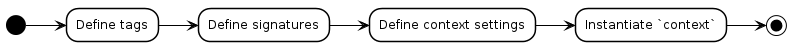
\includegraphics{source/figures/generated/ecst/compiletime/options_activity.png}
\caption{ECST compile-time settings: mandatory options}
\end{figure}

Tag definition was previously described in
\protect\hyperlink{metaprogramming_tags}{Chapter 6, Section 6.2}.
\textbf{Signatures} and \textbf{context settings} will be covered in the
following sections.

\section{Signatures}\label{signatures}

\textbf{Signatures} are
\mintinline[numbersep=12pt, fontsize=\footnotesize, xleftmargin=17pt, linenos, mathescape, bgcolor=codebg]{text}{constexpr}
values containing compile-time options. They are implemented using
option maps, covered in
\protect\hyperlink{metaprogramming_option_maps}{Chapter 6, Section 6.3}.
There are two kinds of signatures: \textbf{component signatures} and
\textbf{system signatures}.

\subsection{Component signatures}\label{component-signatures}

\textbf{Component signatures} are used to \emph{bind} storage strategies
with component types. Multiple component tags can be bound to a specific
storage strategy. Users can implement their own storage strategies
\emph{(briefly explained in
\protect\hyperlink{storage_comp_strategy}{Chapter 9, Subsection
9.1.1})}. The
\mintinline[numbersep=12pt, fontsize=\footnotesize, xleftmargin=17pt, linenos, mathescape, bgcolor=codebg]{text}{contiguous_buffer}
strategy is available by default and allows users to store components in
contiguous memory locations.

\subsubsection{SoA}\label{soa}

Creating a
\mintinline[numbersep=12pt, fontsize=\footnotesize, xleftmargin=17pt, linenos, mathescape, bgcolor=codebg]{text}{contiguous_buffer}
signature per component type results in a \textbf{SoA} \emph{(structure
of arrays)} storage layout:

\begin{minted}[numbersep=12pt, fontsize=\footnotesize, xleftmargin=17pt, linenos, mathescape]{cpp}
namespace cs = ecst::signature::component;

constexpr auto cs_acceleration =
    cs::make(ct::acceleration).contiguous_buffer();

constexpr auto cs_velocity =
    cs::make(ct::velocity).contiguous_buffer();

constexpr auto cs_position =
    cs::make(ct::position).contiguous_buffer();
\end{minted}

\begin{figure}[htbp]
\centering
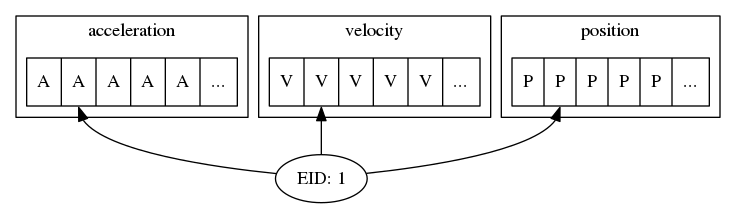
\includegraphics{source/figures/generated/ecst/compiletime/soa_layout.png}
\caption{ECST compile-time settings: high-level view of SoA component
storage layout}
\end{figure}

\subsubsection{AoS}\label{aos}

Creating a
\mintinline[numbersep=12pt, fontsize=\footnotesize, xleftmargin=17pt, linenos, mathescape, bgcolor=codebg]{text}{contiguous_buffer}
signature with multiple component types results in a \textbf{AoS}
\emph{(array of structures)} storage layout:

\begin{minted}[numbersep=12pt, fontsize=\footnotesize, xleftmargin=17pt, linenos, mathescape]{cpp}
constexpr auto cs_physics = signature::component::make(
    ct::acceleration, ct::velocity, ct::position)
        .contiguous_buffer();
\end{minted}

\begin{figure}[htbp]
\centering
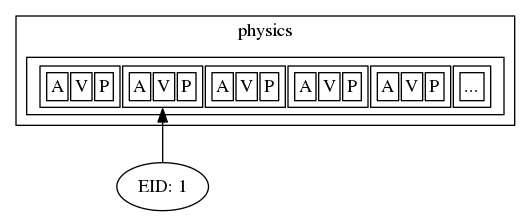
\includegraphics[width=0.75000\textwidth]{source/figures/generated/ecst/compiletime/aos_layout.png}
\caption{ECST compile-time settings: high-level view of AoS component
storage layout}
\end{figure}

\hypertarget{system_sigs}{\subsection{System
signatures}\label{system_sigs}}

\textbf{System signatures} are used to define the following system
settings:

\begin{itemize}
\item
  \textbf{Inner parallelism policy}: either allows the system to run in
  multiple threads \emph{(subtasks)} using a specific strategy or forces
  the system to run in a single thread;
\item
  \textbf{List of dependencies}: list of systems whose execution needs
  to be completed before allowing the current one to run. Used to build
  the \protect\hyperlink{overview_outer_parallelism_dag}{previously
  mentioned} outer parallelism DAG;
\item
  \textbf{Accessed component types}: components types mutated or read by
  the system. Used to subscribe matching entities to the system and to
  allow and verify component access in system implementation;
\item
  \textbf{Output type}: type of data produced by every subtask, if any.
\end{itemize}

An example of a system signature definition is given below:

\begin{minted}[numbersep=12pt, fontsize=\footnotesize, xleftmargin=17pt, linenos, mathescape]{cpp}
constexpr auto ss_collision =
    signature::system::make(st::collision)
        .parallelism(split_evenly_per_core)
        .dependencies(st::spatial_partition)
        .read(ct::circle)
        .write(ct::position, ct::velocity)
        .output(ss::output<std::vector<contact>>);
\end{minted}

\hypertarget{ctopts_siglist}{\subsection{Signature
lists}\label{ctopts_siglist}}

\textbf{Signature lists} are compile-time lists of system signatures,
that are used to group all defined component signatures and system
signatures together, in order to pass them to the context settings
definition.

They are implemented using
\href{http://www.boost.org/doc/libs/1_61_0/libs/hana/doc/html/structboost_1_1hana_1_1basic__tuple.html}{\mintinline[numbersep=12pt, fontsize=\footnotesize, xleftmargin=17pt, linenos, mathescape, bgcolor=codebg]{text}{boost::hana::basic_tuple}}.
The user creates them using the following syntax:

\begin{minted}[numbersep=12pt, fontsize=\footnotesize, xleftmargin=17pt, linenos, mathescape]{cpp}
constexpr auto make_csl()
{
    constexpr auto cs_acceleration = /* ... */;
    constexpr auto cs_velocity = /* ... */;
    constexpr auto cs_position = /* ... */;

    return signature_list::component::make(
        cs_acceleration, cs_velocity, cs_position
        );
}

constexpr auto make_ssl()
{
    constexpr auto ss_acceleration = /* ... */;
    constexpr auto ss_velocity = /* ... */;
    constexpr auto ss_collision = /* ... */;

    return signature_list::system::make(
        ss_acceleration, ss_velocity, ss_collision
        );
}
\end{minted}

\section{Context settings}\label{context-settings}

\textbf{Context settings} are mandatory options that need to be defined
prior to
\mintinline[numbersep=12pt, fontsize=\footnotesize, xleftmargin=17pt, linenos, mathescape, bgcolor=codebg]{text}{context}
instantiation, implemented using
\protect\hyperlink{metaprogramming_option_maps}{option maps}. The
context needs to be aware of:

\begin{itemize}
\item
  All the previously defined \emph{component signatures}, and
  \emph{system signatures}. These will be passed to the settings as
  \emph{signature lists};
\item
  The chosen \textbf{multithreading policy} and \textbf{system
  scheduling strategy};
\item
  The desired \textbf{entity storage policy}, which can be
  \emph{dynamic} or \emph{fixed}.

  \begin{itemize}
  \tightlist
  \item
    Entity and component insertion will be faster with a fixed limit, as
    no checks for possible reallocations are required.
  \end{itemize}
\end{itemize}

Here is an example context settings definition and context
instantiation:

\begin{minted}[numbersep=12pt, fontsize=\footnotesize, xleftmargin=17pt, linenos, mathescape]{cpp}
constexpr auto context_settings =
    ecst::settings::make()
        .allow_inner_parallelism()
        .fixed_entity_limit(ecst::sz_v<10000>)
        .component_signatures(make_csl())
        .system_signatures(make_ssl());

auto context = ecst::context::make(context_settings);
\end{minted}

\hypertarget{chap_flow}{\chapter{Execution flow}\label{chap_flow}}

Using ECST requires the user to follow a particular \textbf{execution
flow}, composed of different stages. The execution flow restricts
possible operations \emph{(using \protect\hyperlink{chap_proxies}{proxy
objects})} in order to keep the state of the application consistent and
to avoid a set of race conditions.

Before examining the execution flow, \textbf{critical operations} will
be defined in the following section.

\section{Critical operations}\label{critical-operations}

Some of the actions that can be executed in specific stages of the
execution flow are called \textbf{critical operations}. These operations
may require \textbf{memory allocations} and/or \textbf{synchronization}
- they have to be executed sequentially. Execution of critical
operations can happen immediately in some contexts \emph{(e.g.~during a
\textbf{step})} or can be delayed using \textbf{deferred functions} in
other contexts \emph{(e.g.~system execution)}.

Critical operations include:

\begin{itemize}
\item
  Creating or destroying an entity;
\item
  Adding or removing a component to/from an entity;
\item
  Starting the execution of a system chain.
\end{itemize}

Non-critical operations include:

\begin{itemize}
\item
  Using a system's output data;
\item
  Marking an entity as \emph{``dead''};
\item
  Accessing or mutating existing component data.
\end{itemize}

An example containing critical and non-critical operations in a system
implementation is shown below:

\begin{minted}[numbersep=12pt, fontsize=\footnotesize, xleftmargin=17pt, linenos, mathescape]{cpp}
template <typename TData>
void process_collision_particles(TData& data)
{
    data.for_entities([&](auto eid)
        {
            // Reading/mutating components is a
            // non-critical operation.
            const auto& contact_list =
                data.get(ct::contact, eid);

            for(const auto& c : contact_list)
            {
                // Critical operation can be delayed
                // to a later stage.
                data.defer([&](auto& proxy)
                    {
                        // Creating entities and adding
                        // or removing components is a
                        // critical operation.
                        auto p = proxy.create_entity();
                        proxy.add_component(ct::particle, p);
                    });
            }

            if(!contact_list.empty())
            {
                // Marking an entity as "dead" is a
                // non-critical operation.
                data.kill_entity(eid);
            }
        });
}
\end{minted}

\section{Flow stages}\label{flow-stages}

ECST's execution flow is composed of the following stages:
\textbf{step}, \textbf{system execution}, \textbf{refresh}.

\hypertarget{step_stage}{\subsection{Step}\label{step_stage}}

\textbf{Step} stages are accessed through a
\mintinline[numbersep=12pt, fontsize=\footnotesize, xleftmargin=17pt, linenos, mathescape, bgcolor=codebg]{text}{context},
using a \textbf{step proxy}.

They:

\begin{itemize}
\item
  Allow immediate execution of \emph{non-critical operations};
\item
  Allow immediate execution of \emph{critical operations};
\item
  Allow execution of system chains;
\item
  Execute a \textbf{refresh} after completion.
\end{itemize}

\begin{figure}[htbp]
\centering
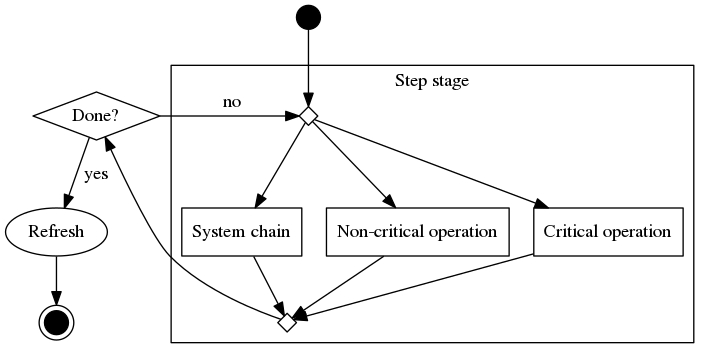
\includegraphics[width=0.90000\textwidth]{source/figures/generated/ecst/flow/stepact.png}
\caption{ECST flow: ``step'' stage overview}
\end{figure}

\subsubsection{User code}\label{user-code}

A step can be defined in user code by calling
\mintinline[numbersep=12pt, fontsize=\footnotesize, xleftmargin=17pt, linenos, mathescape, bgcolor=codebg]{text}{context::step(...)}
with a function that accepts a \emph{step proxy}. The following example
shows a code snippet in which the user, inside of a step stage, prepares
a rendering system, executes a system chain that processes physics and
generates vertices, and finally renders the generated vertices to the
window.

\begin{minted}[numbersep=12pt, fontsize=\footnotesize, xleftmargin=17pt, linenos, mathescape]{cpp}
namespace sea = ::ecst::system_execution_adapter;

context.step([&](auto& proxy)
{
    proxy.system(st::render).prepare();

    proxy.execute_systems(
        sea::t(st::physics).for_subtasks(
            [dt](auto& s, auto& data)
            {
                s.process(dt, data);
            }),
        sea::t(st::render).for_subtasks(
            [](auto& s, auto& data)
            {
                s.process(data);
            })
        );

    proxy.for_system_outputs(st::render,
        [&window](auto& s, auto& va)
        {
            window.draw(va.data(), va.size(),
                PrimitiveType::Triangles);
        });
});
\end{minted}

\subsection{System execution}\label{system-execution}

\textbf{System execution} stages are accessed through system
implementations, using a \textbf{data proxy}.

They:

\begin{itemize}
\item
  Allow immediate execution of \emph{non-critical operations};
\item
  Allow deferred execution of \emph{critical operations}.
\end{itemize}

\hypertarget{flow_refresh}{\subsection{Refresh}\label{flow_refresh}}

\textbf{Refresh} stages are automatically executed after the completion
of a \emph{step stage}.

They sequentially perform the following operations:

\begin{enumerate}
\def\labelenumi{\arabic{enumi}.}
\item
  Collects all deferred functions and executes them sequentially.
\item
  Reclaims all entities marked as ``dead'', making the reuse of their
  IDs possible.
\item
  Matches all newly created, destroyed and modified entities to systems,
  subscribing or unsubscribing them.
\end{enumerate}

A \textbf{refresh state} is instantiated at the beginning of the
refresh, that will be used as a buffer in order to allow communication
between all refresh stages. The refresh state contains a set of entity
IDs to reclaim
\mintinline[numbersep=12pt, fontsize=\footnotesize, xleftmargin=17pt, linenos, mathescape, bgcolor=codebg]{text}{to_kill}
and a set of entity IDs to match
\mintinline[numbersep=12pt, fontsize=\footnotesize, xleftmargin=17pt, linenos, mathescape, bgcolor=codebg]{text}{to_match}.

\begin{algorithm}[H]
\caption{ECST flow: refresh algorithm overview}
\footnotesize

\SetKwData{ToKill}{toKill}
\SetKwData{ToMatch}{toMatch}
\SetKwFunction{ExecuteDeferredFunctions}{ExecuteDeferredFunctions}
\SetKwFunction{ReclaimDeadEntities}{ReclaimDeadEntities}
\SetKwFunction{MatchEntitiesToSystems}{MatchEntitiesToSystems}

    \ToKill $\longleftarrow \emptyset$\;
    \ToMatch $\longleftarrow \emptyset$\;
    \BlankLine
    \ExecuteDeferredFunctions{\ToKill, \ToMatch} \tcp*{fills \ToKill and \ToMatch}
    \ReclaimDeadEntities{\ToKill} \tcp*{mutates and reads \ToKill}
    \MatchEntitiesToSystems{\ToMatch} \tcp*{reads \ToMatch}

\end{algorithm}

\hypertarget{flow_exec_dfuncs}{\subsubsection{Deferred function
execution}\label{flow_exec_dfuncs}}

As deferred functions may contain \emph{critical operations}, they need
to be executed sequentially. Deferred functions are produced during
system execution - every \emph{subtask state} has its own deferred
function list.

\begin{algorithm}[H]
\caption{ECST flow: refresh - ExecuteDeferredFunctions}
\footnotesize

\SetKwData{ToKill}{toKill}
\SetKwData{ToMatch}{toMatch}
\SetKwData{I}{i}
\SetKwData{S}{s}
\SetKwData{C}{c}
\SetKwFunction{F}{F}

    \ForEach{instance \I $\in$ context \C}{
        \ForEach{state \S $\in$ instance \I}{
            \ForEach{function \F $\in$ state \S}{
                \tcc{entity deletion mutats \ToKill}
                \tcc{entity creation or component addition/removal mutates \ToMatch}
                \F{\ToKill, \ToMatch}\;
            }
        }
    }

\end{algorithm}

\subsubsection{Dead entity reclamation}\label{dead-entity-reclamation}

During system execution, entities may be marked as ``dead'' by subtasks.
Every \emph{subtask state} contains a \emph{sparse set} of entity IDs
marked as dead.

\begin{algorithm}[H]
\caption{ECST flow: refresh - ReclaimDeadEntities}
\footnotesize

\SetKwData{ToKill}{toKill}
\SetKwData{I}{i}
\SetKwData{S}{s}
\SetKwData{C}{c}
\SetKwData{Eid}{eid}
\SetKwFunction{F}{F}
\SetKwFunction{Unsubscribe}{Unsubscribe}
\SetKwFunction{Reclaim}{Reclaim}

    \tcc{add entities marked during system execution to \ToKill}
    \ForEach{instance \I $\in$ context \C}{
        \ForEach{state \S $\in$ instance \I}{
             \ToKill $\longleftarrow$ \ToKill $\cup$ \S.\ToKill \;
        }
    }

    \BlankLine

    \tcc{unsubscribe dead entities from systems}
    \ForEach(in parallel){instance \I $\in$ context \C}{
        \ForEach{entityID \Eid $\in$ \ToKill}{
            \Unsubscribe{\I, \Eid}\;
        }
    }

    \BlankLine

    \tcc{reclaim IDs for future use}
    \ForEach{entityID \Eid $\in$ \ToKill}{
        \C.\Reclaim{\Eid}
    }

\end{algorithm}

\subsubsection{Entity-system matching}\label{entity-system-matching}

Newly created entities and entities with a mutated component set must be
matched to systems. Checking if an entity matches a system is done by
computing \emph{dense bitset inclusion} between the entity's active
component bitset and the system's required component bitset. Testing
\mintinline[numbersep=12pt, fontsize=\footnotesize, xleftmargin=17pt, linenos, mathescape, bgcolor=codebg]{text}{std::bitset}
inclusion is not part of the Standard Library \emph{(although proposed,
see {[}\protect\hyperlink{ref-isocpp_proposal_p0125r0}{24}{]})} - it can
be implemented using bitwise operators as follows:

\begin{minted}[numbersep=12pt, fontsize=\footnotesize, xleftmargin=17pt, linenos, mathescape]{cpp}
bool matches(component_bitset cb_entity, component_bitset cb_system)
{
    return (cb_system & cb_entity) == cb_system;
}
\end{minted}

A possible intuition for the code snippet above consists in thinking
about systems as \textbf{keys} and entity instances as \textbf{locks}.
If a key \emph{fits in} a lock, the corresponding entity matches the
system.

\begin{figure}[htbp]
\centering
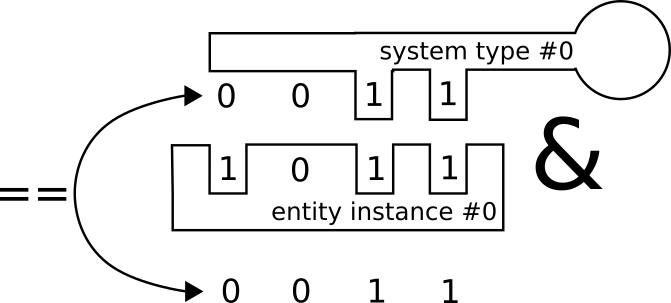
\includegraphics[width=0.85000\textwidth]{source/figures/keylock.png}
\caption{ECST flow: key/lock entity/system matching
intuition}\label{keylock}
\end{figure}

Bitwise inclusion tests can be executed in parallel over all system
instances:

\begin{algorithm}[H]

\caption{ECST flow: refresh - MatchEntitiesToSystems}
\footnotesize

\SetKwData{ToMatch}{toMatch}
\SetKwData{I}{i}
\SetKwData{C}{c}
\SetKwData{Eid}{eid}
\SetKwFunction{Matches}{Matches}
\SetKwFunction{GetComponentBitset}{GetComponentBitset}
\SetKwFunction{Subscribe}{Subscribe}
\SetKwFunction{Unsubscribe}{Unsubscribe}

    \ForEach(in parallel){instance \I $\in$ context \C}{
        \ForEach{entityID \Eid $\in$ \ToMatch}{
            \eIf{\Matches{\GetComponentBitset{\I}, \GetComponentBitset{\Eid}}}{
                \Subscribe{\I, \Eid}\;
            }{
                \Unsubscribe{\I, \Eid}\;
            }
        }
    }

\end{algorithm}

\chapter{Storage}\label{storage}

ECST stores \textbf{entity metadata}, \textbf{component data}, and
\textbf{system instances} inside the context object. To optimize
performance depending on user-defined settings, \emph{static
dispatching} \emph{(see
\protect\hyperlink{appendix_static_dispatching}{Chapter 14, Section
14.3})} techniques are used. This chapter will cover the design and
implementation of the aforementioned storage types.

\hypertarget{storage_component}{\section{Component
data}\label{storage_component}}

Component data is stored in \textbf{chunks}. A \textbf{chunk} binds one
or more component types to a particular \textbf{component storage
strategy}. When the user tries to access a component by a tag
\mintinline[numbersep=12pt, fontsize=\footnotesize, xleftmargin=17pt, linenos, mathescape, bgcolor=codebg]{text}{ct},
the chunk responsible for storing
\mintinline[numbersep=12pt, fontsize=\footnotesize, xleftmargin=17pt, linenos, mathescape, bgcolor=codebg]{text}{ct}
is found at compile-time, and the data is retrieved from the bound
storage.

Chunks are stored inside the context in a
\href{http://www.boost.org/doc/libs/1_61_0/libs/hana/doc/html/structboost_1_1hana_1_1tuple.html}{\mintinline[numbersep=12pt, fontsize=\footnotesize, xleftmargin=17pt, linenos, mathescape, bgcolor=codebg]{text}{boost::hana::tuple}}.

\hypertarget{storage_comp_strategy}{\subsection{Component storage
strategy}\label{storage_comp_strategy}}

A \textbf{component storage strategy} is a class designed to store
component data. Any class can be used as a storage strategy, as long as
it satisfies the following requirements:

\begin{itemize}
\item
  It needs to provide two nested type names:

  \begin{itemize}
  \item
    \mintinline[numbersep=12pt, fontsize=\footnotesize, xleftmargin=17pt, linenos, mathescape, bgcolor=codebg]{text}{component_tag_list_type}:
    a \emph{type list} containing all the tags of components stored;
  \item
    \mintinline[numbersep=12pt, fontsize=\footnotesize, xleftmargin=17pt, linenos, mathescape, bgcolor=codebg]{text}{metadata_type}:
    storage-specific metadata that will be \emph{injected} in entity
    metadata. Can be used to store additional data required to retrieve
    components directly in the entities. Usually an empty class.
  \end{itemize}
\item
  It needs to implement the following interface:

  \begin{minted}[numbersep=12pt, fontsize=\footnotesize, xleftmargin=17pt, linenos, mathescape]{cpp}
  // Given a component tag, an entity ID and its
  // storage-specific metadata, returns a reference to
  // the corresponding component.
  template <typename TComponentTag, typename... Ts>
  auto& get(TComponentTag, entity_id, const metadata_type&);

  // Given a component tag, an entity ID and its
  // storage-specific metadata, creates a component and
  // returns a reference to it.
  template <typename TComponentTag, typename... Ts>
  auto& add(TComponentTag, entity_id, metadata_type&);
  \end{minted}
\end{itemize}

By default, the
\mintinline[numbersep=12pt, fontsize=\footnotesize, xleftmargin=17pt, linenos, mathescape, bgcolor=codebg]{text}{contiguous_buffer},
\mintinline[numbersep=12pt, fontsize=\footnotesize, xleftmargin=17pt, linenos, mathescape, bgcolor=codebg]{text}{empty}
and
\mintinline[numbersep=12pt, fontsize=\footnotesize, xleftmargin=17pt, linenos, mathescape, bgcolor=codebg]{text}{hash_map}
storage strategies are available.

\begin{itemize}
\item
  \mintinline[numbersep=12pt, fontsize=\footnotesize, xleftmargin=17pt, linenos, mathescape, bgcolor=codebg]{text}{contiguous_buffer}
  stores data in either an
  \mintinline[numbersep=12pt, fontsize=\footnotesize, xleftmargin=17pt, linenos, mathescape, bgcolor=codebg]{text}{std::array}
  or an
  \mintinline[numbersep=12pt, fontsize=\footnotesize, xleftmargin=17pt, linenos, mathescape, bgcolor=codebg]{text}{std::vector},
  depending on whether or not the \emph{entity limit} is fixed or
  dynamic.
\item
  \mintinline[numbersep=12pt, fontsize=\footnotesize, xleftmargin=17pt, linenos, mathescape, bgcolor=codebg]{text}{empty}
  does not store any data - it's used for data-less components which
  only ``mark'' entities.
\item
  \mintinline[numbersep=12pt, fontsize=\footnotesize, xleftmargin=17pt, linenos, mathescape, bgcolor=codebg]{text}{hash_map}
  stores data in an
  \mintinline[numbersep=12pt, fontsize=\footnotesize, xleftmargin=17pt, linenos, mathescape, bgcolor=codebg]{text}{std::unordered_map}.
  It should only be used for very big components with infrequent
  lookups/additions.
\end{itemize}

Users can create their own storage strategies by writing classes
fulfilling the requirements mentioned above, and by providing a
\emph{``maker''}
\mintinline[numbersep=12pt, fontsize=\footnotesize, xleftmargin=17pt, linenos, mathescape, bgcolor=codebg]{text}{struct}
with the following interface:

\begin{minted}[numbersep=12pt, fontsize=\footnotesize, xleftmargin=17pt, linenos, mathescape]{cpp}
template <typename TComponentTagList>
struct my_storage_strategy { /* ... */ };

struct my_storage_strategy_maker
{
    // Given context settings and a list of component tags, return
    // an `mp::type_c` wrapping the appropriate storage strategy.
    template <typename TSettings, typename TComponentTagList>
    constexpr auto make_type(TSettings, TComponentTagList) const

    {
        // Static dispatching that depends on `TSettings` and
        // `TComponentTagList` can be performed here to improve
        // performance and memory usage.

        return mp::type_c</* ... */>;
    }
};
\end{minted}

The newly created class can then be used during component signature
definition:

\begin{minted}[numbersep=12pt, fontsize=\footnotesize, xleftmargin=17pt, linenos, mathescape]{cpp}
constexpr auto cs_test_component =
    cs::make(ct::test_component)
        .storage_strategy(my_storage_strategy_maker{});
\end{minted}

Several component storage strategy designs have been analyzed in depth
by Adam Martin {[}\protect\hyperlink{ref-tmachine_compstorage}{25}{]}.

\hypertarget{storage_entity}{\section{Entity
metadata}\label{storage_entity}}

\textbf{Entity metadata} can be accessed through entity IDs and deals
with keeping track of active components, ensuring handle validity and
storing \emph{chunk metadata}.

It is implemented as a simple
\mintinline[numbersep=12pt, fontsize=\footnotesize, xleftmargin=17pt, linenos, mathescape, bgcolor=codebg]{text}{struct}:

\begin{minted}[numbersep=12pt, fontsize=\footnotesize, xleftmargin=17pt, linenos, mathescape]{cpp}
template <typename TComponentBitset, typename TChunkMetadataTuple>
struct metadata : TChunkMetadataTuple
{
    TComponentBitset _bitset;
    counter _counter;
    // ...
};
\end{minted}

\mintinline[numbersep=12pt, fontsize=\footnotesize, xleftmargin=17pt, linenos, mathescape, bgcolor=codebg]{text}{metadata}
derives from
\mintinline[numbersep=12pt, fontsize=\footnotesize, xleftmargin=17pt, linenos, mathescape, bgcolor=codebg]{text}{TChunkMetadataTuple}
in order to take advantage of the \textbf{empty base optimization}
\emph{(EBO)} \emph{(more details at
{[}\protect\hyperlink{ref-cppreference_ebo}{26}{]})}. The stored
\mintinline[numbersep=12pt, fontsize=\footnotesize, xleftmargin=17pt, linenos, mathescape, bgcolor=codebg]{text}{_counter}
is incremented every time an entity IDs is reused - handles that try to
access an entity check if their local counter matches with
\mintinline[numbersep=12pt, fontsize=\footnotesize, xleftmargin=17pt, linenos, mathescape, bgcolor=codebg]{text}{_counter}
to make sure they're not accessing another entity reusing the same ID
{[}\protect\hyperlink{ref-tmachine_eids}{27}{]}.

All entity metadata instances, along with available entity IDs, are
stored in either
\mintinline[numbersep=12pt, fontsize=\footnotesize, xleftmargin=17pt, linenos, mathescape, bgcolor=codebg]{text}{ecst::entity::container::dynamic}
or
\mintinline[numbersep=12pt, fontsize=\footnotesize, xleftmargin=17pt, linenos, mathescape, bgcolor=codebg]{text}{ecst::entity::container::fixed},
depending on the entity limit specified by the user in context settings.

The dynamic storage uses an
\mintinline[numbersep=12pt, fontsize=\footnotesize, xleftmargin=17pt, linenos, mathescape, bgcolor=codebg]{text}{std::vector}
to store metadata and a \emph{dynamic sparse integer set} to store
available IDs. The fixed storage uses an
\mintinline[numbersep=12pt, fontsize=\footnotesize, xleftmargin=17pt, linenos, mathescape, bgcolor=codebg]{text}{std::array}
to store metadata and a \emph{fixed sparse integer set} to store
available IDs - it is faster than the dynamic one as no checks for
growth \emph{(reallocation)} have to be performed.

\textbf{Sparse integer sets} are data structures extremely efficient for
the management of entity IDs. They are analyzed in
\protect\hyperlink{appendix_sparse_integer_sets}{Chapter 14, Section
14.1}.

\hypertarget{storage_system}{\section{Instances and
systems}\label{storage_system}}

User-defined systems are stored inside \textbf{system instances}. Every
system type has a corresponding system instance. All system instances
are stored in the context, in an
\mintinline[numbersep=12pt, fontsize=\footnotesize, xleftmargin=17pt, linenos, mathescape, bgcolor=codebg]{text}{std::tuple},
allowing users and other modules of the library to lookup instances at
compile-time by system type.

\subsection{Instance}\label{instance}

A \textbf{system instance} is composed of the following members:

\begin{itemize}
\item
  An instance of the user-defined system type - systems can be stateful
  \emph{(e.g.~for caching reasons or to store a data structure)} and may
  require storage;
\item
  A \protect\hyperlink{appendix_sparse_integer_sets}{\emph{sparse
  integer set}} of the currently subscribed entity IDs;
\item
  A \emph{dense bitset} of the component types required for system
  subscription \emph{(see
  \protect\hyperlink{appendix_component_bitset_creation}{Chapter 14,
  Section 14.2} for details)};
\item
  A \protect\hyperlink{multithreading_par_executor}{\textbf{parallel
  executor}} object that implements
  \protect\hyperlink{multithreading_inner_par}{\emph{inner
  parallelism}};
\item
  A \textbf{state manager} object that binds a \textbf{state} to every
  \emph{subtask}.
\end{itemize}

\hypertarget{storage_state}{\subsubsection{State}\label{storage_state}}

Every \emph{subtask} has a corresponding \textbf{state}, which stores
the following elements:

\begin{itemize}
\item
  \emph{Output data} optionally generated from the subtask;

  \begin{itemize}
  \item
    The data is set during subtask execution;
  \item
    The data can be read from dependent systems or during a \emph{step}.
  \end{itemize}
\item
  A
  \mintinline[numbersep=12pt, fontsize=\footnotesize, xleftmargin=17pt, linenos, mathescape, bgcolor=codebg]{text}{to_kill}
  sparse integer set, that keeps track of the entities marked as dead
  during subtask execution;

  \begin{itemize}
  \item
    The set is filled during subtask execution;
  \item
    The entities are reclaimed during a \emph{refresh}.
  \end{itemize}
\item
  A
  \mintinline[numbersep=12pt, fontsize=\footnotesize, xleftmargin=17pt, linenos, mathescape, bgcolor=codebg]{text}{std::vector}
  of \textbf{deferred functions}.

  \begin{itemize}
  \item
    The vector is filled during subtask execution;
  \item
    The functions are sequentially executed during a \emph{refresh}.
  \end{itemize}
\end{itemize}

\chapter{Multithreading}\label{multithreading}

Multithreading is used in ECST in the following situations, to
potentially increase the run-time performance of user applications:

\begin{itemize}
\item
  \textbf{Outer parallelism}: system chains independent from each other
  can run in parallel. Implemented with \textbf{system scheduling};
\item
  \textbf{Inner parallelism}: system execution can be split over
  multiple \emph{subtasks}. Implemented with \textbf{inner parallelism
  strategies} and \textbf{slicing};
\item
  \textbf{Refresh}: some operations in the
  \protect\hyperlink{flow_refresh}{refresh stage} can run in parallel.
\end{itemize}

\section{Thread pool}\label{thread-pool}

Execution of operations in separate threads is achieved through a simple
\textbf{thread pool} which consists of a \textbf{lock-free queue} and a
number of \textbf{workers}. Every worker runs on a separate thread and
continuously dequeues \textbf{tasks} from the queue, executing them.

\begin{figure}[htbp]
\centering
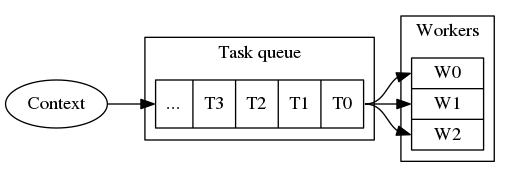
\includegraphics[width=0.75000\textwidth]{source/figures/generated/ecst/multithreading/threadpool.png}
\caption{ECST multithreading: thread-pool architecture}
\end{figure}

Tasks are implemented using
\mintinline[numbersep=12pt, fontsize=\footnotesize, xleftmargin=17pt, linenos, mathescape, bgcolor=codebg]{text}{ecst::fixed_function},
similar to
\mintinline[numbersep=12pt, fontsize=\footnotesize, xleftmargin=17pt, linenos, mathescape, bgcolor=codebg]{text}{std::function}
but with a fixed allocation size. Synchronization is implemented using
\mintinline[numbersep=12pt, fontsize=\footnotesize, xleftmargin=17pt, linenos, mathescape, bgcolor=codebg]{text}{std::condition_variable}
and simple
\mintinline[numbersep=12pt, fontsize=\footnotesize, xleftmargin=17pt, linenos, mathescape, bgcolor=codebg]{text}{std::size_t}
counters. An implementation making use of
\mintinline[numbersep=12pt, fontsize=\footnotesize, xleftmargin=17pt, linenos, mathescape, bgcolor=codebg]{text}{std::packaged_task}
and
\mintinline[numbersep=12pt, fontsize=\footnotesize, xleftmargin=17pt, linenos, mathescape, bgcolor=codebg]{text}{std::future}
was tested, but the unnecessary overhead brought by those classes was
significant.

\subsection{Lock-free queue}\label{lock-free-queue}

To provide \textbf{workers} with tasks, a third-party blocking
concurrent lock-free queue developed by Cameron Desrochers is used. The
queue class is called
\mintinline[numbersep=12pt, fontsize=\footnotesize, xleftmargin=17pt, linenos, mathescape, bgcolor=codebg]{text}{moodycamel::BlockingConcurrentQueue},
and is \href{https://github.com/cameron314/concurrentqueue}{available on
GitHub} under the \emph{Simplified BSD License}.

The queue is used in the worker code as follows:

\begin{minted}[numbersep=12pt, fontsize=\footnotesize, xleftmargin=17pt, linenos, mathescape]{cpp}
void worker::run()
{
    task t;

    while(_state == state::running)
    {
        _queue->wait_dequeue(t);
        t();
    }
}
\end{minted}

The
\mintinline[numbersep=12pt, fontsize=\footnotesize, xleftmargin=17pt, linenos, mathescape, bgcolor=codebg]{text}{_queue->wait_dequeue(t)}
method call will block the current thread until the queue is not empty,
and then dequeue a task into
\mintinline[numbersep=12pt, fontsize=\footnotesize, xleftmargin=17pt, linenos, mathescape, bgcolor=codebg]{text}{t}.
In order to prevent indefinitely waiting upon thread pool destruction, a
number of \emph{``dummy''} empty tasks are spawned to wake up the
waiting workers:

\begin{minted}[numbersep=12pt, fontsize=\footnotesize, xleftmargin=17pt, linenos, mathescape]{cpp}
thread_pool::~thread_pool()
{
    // Signal all workers to exit their processing loops.
    for(auto& w : _workers) w.stop();

    // Post dummy tasks until all workers have exited their loops.
    while(!all_workers_finished()) post_dummy_task();

    // Join the workers' threads.
    for(auto& w : _workers) w.join();
}
\end{minted}

\section{Synchronization}\label{synchronization}

Synchronization and waiting are required when implementing both outer
and inner parallelism:

\begin{itemize}
\item
  When executing outer parallelism, systems must wait for \textbf{all}
  their dependencies to complete before starting execution.
\item
  When executing inner parallelism, \textbf{all} subtasks must be
  finished in order to complete a system execution.
\end{itemize}

The waiting conditions are very simple and can easily and efficiently be
implemented using
\mintinline[numbersep=12pt, fontsize=\footnotesize, xleftmargin=17pt, linenos, mathescape, bgcolor=codebg]{text}{std::condition_variable}
and simple
\mintinline[numbersep=12pt, fontsize=\footnotesize, xleftmargin=17pt, linenos, mathescape, bgcolor=codebg]{text}{std::size_T}
counters. ECST provides a convenient and safe waiting interface,
obtained by wrapping the aforementioned synchronization primitives
alongside an
\mintinline[numbersep=12pt, fontsize=\footnotesize, xleftmargin=17pt, linenos, mathescape, bgcolor=codebg]{text}{std::mutex}
in a class called
\mintinline[numbersep=12pt, fontsize=\footnotesize, xleftmargin=17pt, linenos, mathescape, bgcolor=codebg]{text}{counter_blocker}:

\begin{minted}[numbersep=12pt, fontsize=\footnotesize, xleftmargin=17pt, linenos, mathescape]{cpp}
class counter_blocker
{
private:
    std::condition_variable _cv;
    std::mutex _mutex;
    std::size_t _counter;

public:
    counter_blocker(std::size_t initial_count);

    // Decrements the counter and notifies one waiting thread.
    void decrement_and_notify_one();

    // Decrements the counter and notifies all waiting threads.
    void decrement_and_notify_all();

    // Executes `f` and blocks the caller until the counter
    // reaches zero. Assumes that `f` will trigger a chain of
    // operations that will decrement the counter.
    template <typename TF>
    void execute_and_wait_until_zero(TF&& f);
};
\end{minted}

The
\mintinline[numbersep=12pt, fontsize=\footnotesize, xleftmargin=17pt, linenos, mathescape, bgcolor=codebg]{text}{counter_blocker}
can be used as follows:

\begin{minted}[numbersep=12pt, fontsize=\footnotesize, xleftmargin=17pt, linenos, mathescape]{cpp}
// Create a `counter_blocker` initialized to `n`.
counter_blocker cb{n};

// Immediately execute the passed function and block
// until `cb` reaches zero.
cb.execute_and_wait_until_zero([&]
    {
        // `spawn_tasks` will decrement the counter.
        spawn_tasks(cb, n);
    });
\end{minted}

Here's a possible implementation for
\mintinline[numbersep=12pt, fontsize=\footnotesize, xleftmargin=17pt, linenos, mathescape, bgcolor=codebg]{text}{spawn_tasks}:

\begin{minted}[numbersep=12pt, fontsize=\footnotesize, xleftmargin=17pt, linenos, mathescape]{cpp}
void spawn_tasks(counter_blocker& cb, int n)
{
    for(int i = 0; i < n; ++i)
    {
        post_in_thread_pool([&]
            {
                // Decrement the counter inside `cb` and
                // notify one thread.
                cb.decrement_and_notify_one();
            });
    }
}
\end{minted}

The pattern shown above is used in the implementation of both outer and
inner parallelism and in the refresh stage.

\subsection{Implementation details}\label{implementation-details}

The synchronization operations are hidden behind an interface that takes
a reference to the members of a
\mintinline[numbersep=12pt, fontsize=\footnotesize, xleftmargin=17pt, linenos, mathescape, bgcolor=codebg]{text}{counter_blocker}.
The public methods in
\mintinline[numbersep=12pt, fontsize=\footnotesize, xleftmargin=17pt, linenos, mathescape, bgcolor=codebg]{text}{counter_blocker}
call the following functions:

\begin{minted}[numbersep=12pt, fontsize=\footnotesize, xleftmargin=17pt, linenos, mathescape]{cpp}
// Decrements `c` through `mutex`, and calls `cv.notify_one()`.
void decrement_cv_counter_and_notify_one(
    mutex_type& mutex, cv_type& cv, counter_type& c);

// Decrements `c` through `mutex`, and calls `cv.notify_all()`.
void decrement_cv_counter_and_notify_all(
    mutex_type& mutex, cv_type& cv, counter_type& c);

// Locks `mutex`, executes `f` and waits until `c` is zero
// through `cv`.
template <typename TF>
void execute_and_wait_until_counter_zero(
    mutex_type& mutex, cv_type& cv, counter_type& c, TF&& f);
\end{minted}

The functions above call implementation functions to access the passed
arguments. The most primitive implementation function is
\mintinline[numbersep=12pt, fontsize=\footnotesize, xleftmargin=17pt, linenos, mathescape, bgcolor=codebg]{text}{access_cv_counter},
which calls a passed function after safely accessing the counter inside
a
\mintinline[numbersep=12pt, fontsize=\footnotesize, xleftmargin=17pt, linenos, mathescape, bgcolor=codebg]{text}{counter_blocker}:

\begin{minted}[numbersep=12pt, fontsize=\footnotesize, xleftmargin=17pt, linenos, mathescape]{cpp}
template <typename TF>
void access_cv_counter(
    mutex_type& mutex, cv_type& cv, counter_type& c, TF&& f)
{
    lock_guard_type l(mutex);
    f(cv, c);
}
\end{minted}

It is used as a building block for the \emph{``decrement and notify''}
functions:

\begin{minted}[numbersep=12pt, fontsize=\footnotesize, xleftmargin=17pt, linenos, mathescape]{cpp}
void decrement_cv_counter_and_notify_one(
    mutex_type& m, cv_type& cv, counter_type& c)
{
    access_cv_counter(m, cv, c, [](auto& x_cv, auto& x_c)
        {
            assert(x_c > 0);
            --x_c;
            x_cv.notify_one();
        });
}
\end{minted}

The \emph{``execute and wait''} functions are implemented using an
\mintinline[numbersep=12pt, fontsize=\footnotesize, xleftmargin=17pt, linenos, mathescape, bgcolor=codebg]{text}{std::unique_lock}
waiting on a generic predicate through the
\mintinline[numbersep=12pt, fontsize=\footnotesize, xleftmargin=17pt, linenos, mathescape, bgcolor=codebg]{text}{std::condition_variable}
stored in the
\mintinline[numbersep=12pt, fontsize=\footnotesize, xleftmargin=17pt, linenos, mathescape, bgcolor=codebg]{text}{counter_blocker}:

\begin{minted}[numbersep=12pt, fontsize=\footnotesize, xleftmargin=17pt, linenos, mathescape]{cpp}
template <typename TPredicate, typename TF>
void execute_and_wait_until(
    mutex_type& m, cv_type& cv, TPredicate&& p, TF&& f)
{
    unique_lock_type l(m);
    f();
    cv.wait(l, p);
}

template <typename TF>
void execute_and_wait_until_counter_zero(
    mutex_type& m, cv_type& cv, counter_type& c, TF&& f)
{
    execute_and_wait_until(m, cv,
        [&c]
        {
            return c == 0;
        },
        f);
}
\end{minted}

\section{System scheduling}\label{system-scheduling}

\textbf{System scheduling} implements the concept of \emph{outer
parallelism}. The user can begin system execution during a
\protect\hyperlink{step_stage}{\emph{step stage}} from any number of
independent systems:

\begin{minted}[numbersep=12pt, fontsize=\footnotesize, xleftmargin=17pt, linenos, mathescape]{cpp}
ctx.step([&](auto& proxy)
{
    // Start execution of system chains from `s::s0` and `s::s1`:
    proxy.execute_systems_from(st::s0, st::s1)(
        sea::t(st::s0).for_subtasks([dt](auto& s, auto& data)
            {
                // Overload for `s::s0`.
                s.process(dt, data);
            }),
        sea::t(st::s1).for_subtasks([dt](auto& s, auto& data)
            {
                // Overload for `s::s1`.
                s.process(dt, data);
            }));
});
\end{minted}

The
\mintinline[numbersep=12pt, fontsize=\footnotesize, xleftmargin=17pt, linenos, mathescape, bgcolor=codebg]{text}{s::s0}
and
\mintinline[numbersep=12pt, fontsize=\footnotesize, xleftmargin=17pt, linenos, mathescape, bgcolor=codebg]{text}{s::s1}
system types need to be independent of each other \emph{(a compile-time
error will occur otherwise)}. After calling
\mintinline[numbersep=12pt, fontsize=\footnotesize, xleftmargin=17pt, linenos, mathescape, bgcolor=codebg]{text}{proxy.execute_systems_from},
the \protect\hyperlink{architecture_system_mgr}{system manager} inside
the context will instantiate a system scheduler and begin execution:

\begin{minted}[numbersep=12pt, fontsize=\footnotesize, xleftmargin=17pt, linenos, mathescape]{cpp}
template <typename TSettings>
template <typename TCtx, typename TSystemTagList, typename... TFs>
void system_manager<TSettings>::execute_systems_impl(
    TCtx& ctx, TSystemTagList sstl, TFs&&... fs)
{
    // Instantiate system scheduler (specified in context settings).
    scheduler_type s;

    // Overload user-provided functions.
    auto o_fs = boost::hana::overload_linearly(fs...);

    // Begin execution.
    // (Blocks until all systems in the chain have been executed.)
    s.execute(ctx, sstl, os);
}
\end{minted}

The current only default system scheduler type is called
\mintinline[numbersep=12pt, fontsize=\footnotesize, xleftmargin=17pt, linenos, mathescape, bgcolor=codebg]{text}{atomic_counter}
- it
\mintinline[numbersep=12pt, fontsize=\footnotesize, xleftmargin=17pt, linenos, mathescape, bgcolor=codebg]{text}{counter_blocker}
instances to wait for system dependencies' execution completion.

\hypertarget{mt_ac_scheduler}{\subsection{Atomic counter
scheduler}\label{mt_ac_scheduler}}

The
\mintinline[numbersep=12pt, fontsize=\footnotesize, xleftmargin=17pt, linenos, mathescape, bgcolor=codebg]{text}{atomic_counter}
scheduler keeps count of the remaining systems \emph{(yet to be
executed)} and assigns a \textbf{task} to every system. Every task keeps
count of its \textbf{remaining dependencies}. Tasks are executed
recursively - after completing the starting independent tasks, every
\textbf{dependent task} \emph{(child task)} whose dependencies were
satisfied is executed.

The scheduler will block until all systems have been executed, and all
dependencies between systems will be respected. Here's a high-level
pseudocode of the algorithm:

\begin{algorithm}[H]

\caption{ECST multithreading: system scheduler - atomic counter}
\footnotesize

\SetKwFunction{GetChainSize}{GetChainSize}
\SetKwData{StartTags}{startSystems}
\SetKwData{CurrentSystems}{currentSystems}
\SetKwData{RemainingSystems}{remainingSystems}

\SetKwFunction{ExecuteSystems}{ExecuteSystems}
\SetKwFunction{RunChain}{RunTask}
\SetKwFunction{TaskFromSystem}{TaskFromSystem}
\SetKwFunction{SystemOf}{SystemOf}
\SetKwFunction{DependentTasks}{DependentTasks}
\SetKwFunction{DecrementAtomicCounter}{DecrementAtomicCounter}

\SetKwFunction{DecrementRemainingDependencies}{DecrementRemainingDependencies}
\SetKwFunction{RemainingDependenciesCount}{RemainingDependenciesCount}

\SetKwInOut{Input}{input}\SetKwInOut{Output}{output}

\SetKwBlock{BlockWhile}{}{end}
\SetKw{BlockWhileKw}{block thread while}
\SetKw{KwEnd}{end}

\SetKwData{T}{t}
\SetKwData{Dt}{dt}
\SetKwData{S}{s}
\SetKwData{F}{f}


\Input{List of starting system tags \StartTags}
\Input{Overloaded processing function \F}

\SetKwFunction{algo}{algo}\SetKwFunction{proc}{proc}
\SetKwProg{myalg}{Algorithm}{}{}

\SetAlgoLined

    \BlankLine

    \myalg{\ExecuteSystems{\StartTags, \F}}{
        \tcc{count unique nodes traversed from every starting system}
        \RemainingSystems $\longleftarrow$ \GetChainSize{\StartTags}\;

        \BlankLine

        \tcc{start recursive task execution}
        \ForEach(in parallel){system \S $\in$ \StartTags}{
            \T $\longleftarrow$ \TaskFromSystem{\S}\;
            \RunChain{\RemainingSystems, \T, \F}\;
        }

        \BlankLine

        \tcc{block until all systems have been executed}
        \BlockWhileKw \RemainingSystems $> 0$\;
    }
    \KwEnd

    \BlankLine
    \BlankLine

    \SetKwProg{myproc}{Procedure}{}{}
    \myproc{\RunChain{\RemainingSystems, \T, \F}}{

        \tcc{execute current task}
        \F{\SystemOf{\T}}\;
        \DecrementAtomicCounter{\RemainingSystems}\;
        \BlankLine


        \tcc{for each dependent child task}
        \ForEach{task \Dt $\in$ \DependentTasks{\T}}{

            \tcc{notify \Dt the current (parent) task was executed}
            \DecrementRemainingDependencies{\Dt}\;

            \BlankLine

            \tcc{run \Dt recursively if its dependencies were satisfied}

            \If{\RemainingDependenciesCount{\Dt} $ == 0$}{
                \RunChain{\RemainingSystems, \Dt, \F}\;
            }
        }
    }
    \KwEnd

\end{algorithm}

The implementation of the algorithm above will be now analyzed in the
sections below.

\hypertarget{mt_s_sce}{\subsubsection{Starting chain
execution}\label{mt_s_sce}}

The first step is traversing the implicit dependency \textbf{directed
acyclic graph}, from every user-provided starting system type, counting
the unique traversed nodes. This is done with a compile-time
\protect\hyperlink{appendix_compiletime_bfs}{\textbf{breadth-first
traversal}}.

\begin{minted}[numbersep=12pt, fontsize=\footnotesize, xleftmargin=17pt, linenos, mathescape]{cpp}
template <typename TCtx, typename TSystemTagList, typename TF>
void atomic_counter::execute(TCtx& ctx, TSystemTagList sstl, TF&& f)
{
    // Count of nodes traversed starting from every node in `sstl`.
    constexpr auto n = signature_list::system::chain_size(ssl, sstl);

    // Counter blocker used to block until all systems in the chain
    // have been executed.
    counter_blocker b{n};

    // Begin the execution and block until all systems have finished.
    b.execute_and_wait_until_zero([&]() mutable
        {
            this->start_execution(ctx, sstl, b, f);
        });
}
\end{minted}

\mintinline[numbersep=12pt, fontsize=\footnotesize, xleftmargin=17pt, linenos, mathescape, bgcolor=codebg]{text}{atomic_counter::start_execution}
will begin the recursive task execution.

\hypertarget{multithreading_recursive_task_execution}{\subsubsection{Recursive
task execution}\label{multithreading_recursive_task_execution}}

Every system in the context has an assigned task, which has a unique ID.
\mintinline[numbersep=12pt, fontsize=\footnotesize, xleftmargin=17pt, linenos, mathescape, bgcolor=codebg]{text}{atomic_counter::start_execution}
retrieves the tasks of the starting systems and executes them
recursively:

\begin{minted}[numbersep=12pt, fontsize=\footnotesize, xleftmargin=17pt, linenos, mathescape]{cpp}
template <typename TCtx, typename TSystemTagList, typename TBlocker,
    typename TF>
void atomic_counter::start_execution(
    TCtx& ctx, TSystemTagList sstl, TBlocker& b, TF&& f)
{
    // For each system tag in `sstl`...
    boost::hana::for_each(sstl, [&](auto st) mutable
        {
            // Get the corresponding task ID.
            auto sid = sls::id_by_tag(this->ssl(), st);

            // Run task with ID `sid`.
            ctx.post_in_thread_pool([&]() mutable
                {
                    this->task_by_id(sid).run(b, id, sp, f);
                });
        });
}
\end{minted}

After retrieving a task by ID,
\mintinline[numbersep=12pt, fontsize=\footnotesize, xleftmargin=17pt, linenos, mathescape, bgcolor=codebg]{text}{atomic_counter::task::run}
will effectively execute the overloaded user-provided processing
function on the system and recursively run children tasks with no
remaining dependencies:

\begin{minted}[numbersep=12pt, fontsize=\footnotesize, xleftmargin=17pt, linenos, mathescape]{cpp}
template <typename TBlocker, typename TID, typename TCtx, typename TF>
void atomic_counter::task::run(TBlocker& b, TID sid, TCtx& ctx, TF&& f)
{
    // Get reference to system instance from task ID.
    auto& s_instance(ctx.instance_by_id(sid));

    // Execute overloaded processing function on system instance.
    s_instance.execute(ctx, f);

    // Safely decrement "remaining systems" counter.
    b.decrement_and_notify_one();

    // For every dependent task ID...
    for_dependent_ids([&](auto id)
        {
            // Retrieve the corresponding task.
            auto& dt = task_by_id(id);

            // Then, inform the task that one of its dependencies (the
            // current task) has been executed.
            dt.decrement_remaining_dependencies();

            if(dt.remaining_dependencies() == 0)
            {
                // Recursively run the dependent task.
                ctx.post_in_thread_pool([&]
                    {
                        dt.run(b, id, ctx, f);
                    });
            }
        });
}
\end{minted}

\hypertarget{multithreading_inner_par}{\section{Inner
parallelism}\label{multithreading_inner_par}}

\textbf{Inner parallelism} allows single systems to be run in parallel
by \emph{splitting} the range of their subscribed entities across a
number of \textbf{subtasks}. Every subtask has its own \textbf{state}
and can run in a separate thread. \textbf{Parallel executors}, which are
obtained by composing \textbf{inner parallelism strategies}, implement
the concept of \emph{inner parallelism}.

\hypertarget{multithreading_par_executor}{\subsection{Parallel
executor}\label{multithreading_par_executor}}

Every \emph{system instance} stores a \textbf{parallel executor}.
Parallel executors wrap inner parallelism strategies composed at
compile-time by library users. Here is an example definition of an inner
parallelism strategy:

\begin{minted}[numbersep=12pt, fontsize=\footnotesize, xleftmargin=17pt, linenos, mathescape]{cpp}
namespace ips = ecst::inner_parallelism::strategy;
namespace ipc = ecst::inner_parallelism::composer;

constexpr auto my_parallelism_strategy =
    ipc::none_below_threshold::v(sz_v<10000>,
        ips::split_evenly_fn::v_cores()
        );

constexpr auto ss_acceleration =
    ss::make(st::acceleration)
        .parallelism(my_parallelism_strategy)
        .read(ct::acceleration)
        .write(ct::velocity);
\end{minted}

The code snippet above configures
\mintinline[numbersep=12pt, fontsize=\footnotesize, xleftmargin=17pt, linenos, mathescape, bgcolor=codebg]{text}{s::acceleration}
to run in a single thread if its subscriber count is less than
\(10000\), otherwise it will be evenly split across the available CPU
cores.

System instances invoke the parallel executor by passing a reference to
the parent context and a \textbf{subtask adapter} function. The subtask
adapter function for parallel execution takes the following arguments:

\begin{itemize}
\item
  \textbf{Split index}, which is the ID of the current subtask.
\item
  Begin and end \textbf{slice indices}, which will be stored inside a
  \protect\hyperlink{dddata_proxy}{data proxy}. They are used to
  retrieve the target entity subset.
\end{itemize}

\begin{minted}[numbersep=12pt, fontsize=\footnotesize, xleftmargin=17pt, linenos, mathescape]{cpp}
template <typename TContext, typename TF>
void instance</* ... */>::execute_in_parallel(TContext& ctx, TF&& f)
{
    // "Subtask adapter" lambda.
    auto st = [&](auto split_idx, auto i_begin, auto i_end)
    {
        // Create multi data proxy.
        auto dp = data_proxy::make_multi<TSystemSignature>(
            *this, ctx, split_idx, i_begin, i_end);

        // Execute the bound slice.
        f(dp);
    };

    _parallel_executor.execute(*this, ctx, std::move(st));
}
\end{minted}

This design has been chosen in order to easily implement other system
instance types in the future \emph{(e.g.~systems that directly process
component data, without knowledge of entities)}. The parallel executor
implementation will ask the caller instance to prepare execution of
\(n\) subtasks:

\begin{minted}[numbersep=12pt, fontsize=\footnotesize, xleftmargin=17pt, linenos, mathescape]{cpp}
template <typename TInstance, typename TCtx, typename TF>
void split_every_n</* ... */>::execute(
    TInstance& i, TCtx& ctx, TF&& f)
{
    // Perform strategy-related calculations.
    auto per_split = /* ... */;
    auto split_count = /* ... */;

    // Executes all subtasks. Blocks until completed.
    utils::prepare_execute_wait_subtasks(
       inst, ctx, split_count, per_split, f);
}
\end{minted}

The
\mintinline[numbersep=12pt, fontsize=\footnotesize, xleftmargin=17pt, linenos, mathescape, bgcolor=codebg]{text}{utils::prepare_execute_wait_subtasks}
function takes care of calling the
\mintinline[numbersep=12pt, fontsize=\footnotesize, xleftmargin=17pt, linenos, mathescape, bgcolor=codebg]{text}{instance::prepare_and_wait_subtasks}
method, which initializes the
\mintinline[numbersep=12pt, fontsize=\footnotesize, xleftmargin=17pt, linenos, mathescape, bgcolor=codebg]{text}{counter_blocker}
with the number of produced subtasks and starts their execution. The
method performs the following operations:

\begin{itemize}
\item
  It \textbf{clears} and \textbf{prepares} the
  \protect\hyperlink{storage_state}{\emph{states}} necessary for subtask
  execution.
\item
  It instantiates a
  \mintinline[numbersep=12pt, fontsize=\footnotesize, xleftmargin=17pt, linenos, mathescape, bgcolor=codebg]{text}{counter_blocker}
  that will block until all subtasks have been executed.
\item
  It creates an adapter \emph{``run in separate thread''} function that
  will be used to run all subtasks except one in separate thread pool
  tasks. This will allow the current thread to execute one of the
  subtasks.
\end{itemize}

\begin{minted}[numbersep=12pt, fontsize=\footnotesize, xleftmargin=17pt, linenos, mathescape]{cpp}
template <typename TContext, typename TF>
void instance</* ... */>::prepare_and_wait_n_subtasks(
    TContext& ctx, int n, TF&& f)
{
    // Prepare `n` states, but set the counter to `n - 1` since one
    // of the subtasks will be executed in the current thread.
    _sm.clear_and_prepare(n);
    counter_blocker b{n - 1};

    // Function accepting a callable object which will be executed
    // in a separate thread. Intended to be called from inner
    // parallelism strategy executors.
    auto run_in_separate_thread = [this, &ctx, &b](auto& xf)
    {
        return [this, &b, &ctx, &xf](auto&&... xs)
        {
            ctx.post_in_thread_pool([&xf, &b, xs...]()
                {
                    xf(xs...);
                    b.decrement_and_notify_all();
                });
        };
    };

    // Runs the parallel executor and waits until the remaining
    // subtasks counter is zero.
    b.execute_and_wait_until_zero([&f, &run_in_separate_thread]
        {
            f(run_in_separate_thread);
        });
}
\end{minted}

\hypertarget{chap_proxies}{\chapter{Proxy objects}\label{chap_proxies}}

\textbf{Proxy objects} are used to provide the user with a
\emph{restricted interface} that increases the safety and readability of
application code. Proxy objects are instantiated by ECST and passed as a
reference in the following cases:

\begin{itemize}
\item
  During entity processing in systems, a \textbf{data proxy} object is
  used to access \emph{component data} and \emph{previous system
  outputs}.

  \begin{itemize}
  \tightlist
  \item
    Data proxies also give access to \emph{deferred function} creation,
    which is done through \textbf{defer proxy} objects. Defer proxies
    allow the user to enqueue \emph{critical operations} in a context
    where only non-critical operations can be executed.
  \end{itemize}
\item
  In order to immediately execute \emph{critical operations} or begin
  \emph{system chain execution}, a \textbf{step proxy} object must be
  used. Step proxies are created from the context and accessed through
  the
  \mintinline[numbersep=12pt, fontsize=\footnotesize, xleftmargin=17pt, linenos, mathescape, bgcolor=codebg]{text}{context::step}
  method.

  \begin{itemize}
  \tightlist
  \item
    \textbf{Executor proxy} objects are required to access \emph{system
    processing functions} during system chain execution \emph{(inside of
    a \textbf{step})}. They are usually hidden behind more convenient
    abstractions provided by \emph{system execution adapters}.
  \end{itemize}
\end{itemize}

All proxies are implemented as template classes containing
\mintinline[numbersep=12pt, fontsize=\footnotesize, xleftmargin=17pt, linenos, mathescape, bgcolor=codebg]{text}{private}
callable objects \emph{(and additional data)}, with a
\mintinline[numbersep=12pt, fontsize=\footnotesize, xleftmargin=17pt, linenos, mathescape, bgcolor=codebg]{text}{public}
interface that invokes the stored callables.

\hypertarget{dddata_proxy}{\section{Data proxies}\label{dddata_proxy}}

\textbf{Data proxies} are created during
\protect\hyperlink{inner_par_slicing}{\emph{inner parallelism slicing}}.
Every data proxy is bound to a particular
\protect\hyperlink{storage_state}{\emph{subtask state}} and provides the
following interface functions:

\begin{itemize}
\item
  Entity iteration:

  \begin{minted}[numbersep=12pt, fontsize=\footnotesize, xleftmargin=17pt, linenos, mathescape]{cpp}
  // Iterates over entities assigned to the current subtask.
  template <typename TF>
  auto for_entities(TF&& f);

  // Iterates over all entities in the system.
  template <typename TF>
  auto for_all_entities(TF&& f);

  // Iterates over all entities not in the current subtask.
  template <typename TF>
  auto for_other_entities(TF&& f);
  \end{minted}
\item
  Entity count:

  \begin{minted}[numbersep=12pt, fontsize=\footnotesize, xleftmargin=17pt, linenos, mathescape]{cpp}
  // Count of entities of the current subtask.
  auto entity_count() const;

  // Count of all entities in the system.
  auto all_entity_count() const;

  // Count of entities not in the current subtask.
  auto other_entity_count() const;
  \end{minted}
\item
  Entity/component manipulation:

  \begin{minted}[numbersep=12pt, fontsize=\footnotesize, xleftmargin=17pt, linenos, mathescape]{cpp}
  // Returns a reference to a component of `eid` with tag `ct`.
  template <typename TComponentTag>
  decltype(auto) get(TComponentTag ct, entity_id eid);

  // Enqueues a "deferred function".
  template <typename TF>
  void defer(TF&& f);

  // Marks an entity as "dead".
  void kill_entity(entity_id eid);
  \end{minted}
\item
  System output access:

  \begin{minted}[numbersep=12pt, fontsize=\footnotesize, xleftmargin=17pt, linenos, mathescape]{cpp}
  // Returns a reference to the system's output data.
  auto& output();

  // Loops over the outputs of a previous system (dependency).
  template <typename TSystemTag, typename TF>
  decltype(auto) for_previous_outputs(TSystemTag st, TF&& f);
  \end{minted}
\end{itemize}

Data proxies begin their life during the definition of system processing
overloads \emph{(in a \textbf{step})}:

\begin{minted}[numbersep=12pt, fontsize=\footnotesize, xleftmargin=17pt, linenos, mathescape]{cpp}
ctx.step([&](auto& proxy)
    {
        proxy.execute_systems_from(st::s0, st::s1)(
            sea::t(st::s0).for_subtasks([](auto& s, auto& data)
                {
                    s.process(data);
                }),
            sea::t(st::s1).for_subtasks([](auto& s, auto& data)
                {
                    s.process(data);
                }));
    });
\end{minted}

The
\mintinline[numbersep=12pt, fontsize=\footnotesize, xleftmargin=17pt, linenos, mathescape, bgcolor=codebg]{text}{data}
arguments shown above are created during
\protect\hyperlink{inner_par_slicing}{\emph{inner parallelism slicing}}
and automatically passed to the overloaded processing functions by the
context. The system implementation can then access data proxies as
follows:

\begin{minted}[numbersep=12pt, fontsize=\footnotesize, xleftmargin=17pt, linenos, mathescape]{cpp}
struct s0
{
    template<typename TData>
    void process(TData& data)
    {
        data.for_entities([](auto eid){ /* ... */ });
    }
};
\end{minted}

\hypertarget{proxies_defer}{\subsection{Defer
proxies}\label{proxies_defer}}

\textbf{Defer proxies} are created by data proxies and can only be
accessed through them. They provide an interface to enqueue critical
operations that will be executed during a
\protect\hyperlink{flow_refresh}{\emph{refresh}}:

\begin{itemize}
\item
  Entity/handle manipulation:

  \begin{minted}[numbersep=12pt, fontsize=\footnotesize, xleftmargin=17pt, linenos, mathescape]{cpp}
  entity_id create_entity();
  void kill_entity(entity_id);

  handle create_handle(entity_id);
  handle create_entity_and_handle();
  auto valid_handle(const handle& h) const;
  auto access(const handle&) const;
  \end{minted}
\item
  Component access/manipulation:

  \begin{minted}[numbersep=12pt, fontsize=\footnotesize, xleftmargin=17pt, linenos, mathescape]{cpp}
  template <typename TComponentTag>
  decltype(auto) add_component(TComponentTag, entity_id);

  template <typename TComponentTag>
  decltype(auto) get_component(TComponentTag, entity_id);

  template <typename TComponentTag>
  void remove_component(TComponentTag, entity_id);
  \end{minted}
\item
  System access:

  \begin{minted}[numbersep=12pt, fontsize=\footnotesize, xleftmargin=17pt, linenos, mathescape]{cpp}
  template <typename TSystemTag>
  auto& instance(TSystemTag);

  template <typename TSystemTag>
  auto& system(TSystemTag);

  template <typename TSystemTag, typename TF>
  decltype(auto) for_system_outputs(TSystemTag, TF&& f);
  \end{minted}
\end{itemize}

Here is an example of a defer proxy in use:

\begin{minted}[numbersep=12pt, fontsize=\footnotesize, xleftmargin=17pt, linenos, mathescape]{cpp}
data.for_entities([&](auto eid)
    {
        data.defer([&](auto& proxy)
            {
                auto e = proxy.create_entity();
                proxy.add_component(ct::c0, e);
            });
    });
\end{minted}

The enqueued operations will be executed at the end of a
\protect\hyperlink{step_stage}{\emph{step}}, during the
automatically-triggered \protect\hyperlink{flow_exec_dfuncs}{refresh
\emph{``execute deferred functions''} phase}.

\hypertarget{proxies_step}{\section{Step proxies}\label{proxies_step}}

\textbf{Step proxies} allow every operation that
\protect\hyperlink{proxies_defer}{\emph{defer proxies}} do, in addition
to functions which \emph{begin system chain execution}:

\begin{minted}[numbersep=12pt, fontsize=\footnotesize, xleftmargin=17pt, linenos, mathescape]{cpp}
// Executes all system chains starting from `sts...`.
template <typename... TStartSystemTags>
auto execute_systems_from(TStartSystemTags... sts);

// Executes all system chains.
auto execute_systems();
\end{minted}

These functions are accessed through the
\mintinline[numbersep=12pt, fontsize=\footnotesize, xleftmargin=17pt, linenos, mathescape, bgcolor=codebg]{text}{context::step}
method, which creates a step proxy and passes it to an user-defined
function. The method also accepts a variadic number of
\mintinline[numbersep=12pt, fontsize=\footnotesize, xleftmargin=17pt, linenos, mathescape, bgcolor=codebg]{text}{fs_refresh...}
refresh event handler functions: the feature will be covered in
\protect\hyperlink{chap_advfeats}{Chapter 12, Section 12.1}.

\begin{minted}[numbersep=12pt, fontsize=\footnotesize, xleftmargin=17pt, linenos, mathescape]{cpp}
template <typename TFStep, typename... TFsRefresh>
auto context::step(TFStep&& f_step, TFsRefresh&&... fs_refresh)
{
    auto refresh_event_handler =
        boost::hana::overload_linearly(fs_refresh...);

    // Ensure `refresh()` is automatically called after executing `f`.
    ECST_SCOPE_GUARD([this, reh = std::move(refresh_event_handler)]
        {
            this->refresh(std::move(reh));
        });

    // Clear refresh state.
    _refresh_state.clear();

    // Build context step proxy.
    step_proxy_type step_proxy{*this, _refresh_state};

    // Execute user-defined step.
    return f_step(step_proxy);
}
\end{minted}

Here is an example usage of a step proxy:

\begin{minted}[numbersep=12pt, fontsize=\footnotesize, xleftmargin=17pt, linenos, mathescape]{cpp}
ctx.step([&](auto& proxy)
    {
        proxy.execute_systems()(
            sea::all().for_subtasks([](auto& s, auto& data)
                {
                    s.process(data);
                }));
    },
    ecst::refresh_event::on_unsubscribe(st::s0,
        [](s::s0& system, entity_id eid){ /* ... */ }));
\end{minted}

\subsection{Executor proxies}\label{executor-proxies}

\textbf{Executor proxies} are created from \emph{system instances} and
used to execute system processing functions. They allow more
fine-grained control over system execution and can only be accessed in a
\emph{step}, using the
\mintinline[numbersep=12pt, fontsize=\footnotesize, xleftmargin=17pt, linenos, mathescape, bgcolor=codebg]{text}{.detailed}
method of any \emph{system execution adapter}. Here's a usage example:

\begin{minted}[numbersep=12pt, fontsize=\footnotesize, xleftmargin=17pt, linenos, mathescape]{cpp}
ctx.step([](auto& proxy)
    {
        proxy.execute_systems()(
            sea::all().detailed([&](auto& system, auto& executor)
                {
                    // Code to run before execution.

                    executor.for_subtasks([&](auto& data)
                        {
                            // Code that runs in every subtask.
                            system.process(data);
                        });

                    // Code to run after execution.
                }));
    });
\end{minted}

Normally, executor proxies are hidden behind the more convenient
\emph{(yet more limited)} \emph{system execution adapter}
\mintinline[numbersep=12pt, fontsize=\footnotesize, xleftmargin=17pt, linenos, mathescape, bgcolor=codebg]{text}{.for_subtasks}
method interface.

\hypertarget{chap_advfeats}{\chapter{Advanced
features}\label{chap_advfeats}}

This chapter will cover the design and implementation of some less
commonly used ECST features.

\hypertarget{advf_refresh_event_handling}{\section{Refresh event
handling}\label{advf_refresh_event_handling}}

The \protect\hyperlink{flow_refresh}{refresh stage} takes care of
various important operations, such as reclaiming dead entity IDs and
subscribing/unsubscribing entities to systems. These operations produce
\emph{events} that can be optionally handled by the user through
\textbf{refresh event handling}.

When calling the
\mintinline[numbersep=12pt, fontsize=\footnotesize, xleftmargin=17pt, linenos, mathescape, bgcolor=codebg]{text}{context::step}
method, a variadic number of functions can be passed that will be
overloaded to \emph{catch} refresh events and execute code:

\begin{minted}[numbersep=12pt, fontsize=\footnotesize, xleftmargin=17pt, linenos, mathescape]{cpp}
ctx.step([](auto& proxy){ /* ... */ },
    ecst::refresh_event::on_unsubscribe(st::s0,
        [](auto& instance, auto eid)
        {
            // Handle unsubscription of `eid` from `s::s0`.
        }),
    ecst::refresh_event::on_subscribe(st::s1,
        [](auto& instance, auto eid)
        {
            // Handle subscription of `eid` from `s::s1`.
        }),
    ecst::refresh_event::on_reclaim([](auto eid)
        {
            // Handle reclamation of `eid`.
        }));
\end{minted}

\subsection{Implementation details}\label{implementation-details-1}

Refresh event handling is completely optional and implemented with
compile-time function overloading: it does not introduce any additional
unnecessary run-time overhead:

\begin{minted}[numbersep=12pt, fontsize=\footnotesize, xleftmargin=17pt, linenos, mathescape]{cpp}
template <typename TFStep, typename... TFsRefresh>
auto context::step(TFStep&& f_step, TFsRefresh&&... fs_refresh)
{
    // Creates the overload of refresh event handlers...
    auto refresh_event_handler =
        boost::hana::overload_linearly(fs_refresh...);

    ECST_SCOPE_GUARD([this, reh = std::move(refresh_event_handler)]
        {
            // ...and passes it to refresh.
            this->refresh(std::move(reh));
        });

    // ...
}
\end{minted}

Every event has a unique type and
\mintinline[numbersep=12pt, fontsize=\footnotesize, xleftmargin=17pt, linenos, mathescape, bgcolor=codebg]{text}{constexpr}
variable:

\begin{minted}[numbersep=12pt, fontsize=\footnotesize, xleftmargin=17pt, linenos, mathescape]{cpp}
namespace impl
{
    struct subscribed_t { };
    struct unsubscribed_t { };
    struct reclaimed_t { };

    constexpr subscribed_t subscribed{};
    constexpr unsubscribed_t unsubscribed{};
    constexpr reclaimed_t reclaimed{};
}
\end{minted}

Refresh implementation stages invoke the created overloaded function
using the types defined above, in order to trigger the correct overload.
Here is an example:

\begin{minted}[numbersep=12pt, fontsize=\footnotesize, xleftmargin=17pt, linenos, mathescape]{cpp}
void context::refresh_impl_kill_entities(
    TRefreshState& rs, TFRefresh&& f_refresh)
{
    // ...

    // Reclaim all dead entities and fire events.
    rs._to_kill.for_each([&](entity_id eid)
        {
            this->reclaim(eid);
            f_refresh(refresh_event::impl::reclaimed, eid);
        });

    // ...
}

\end{minted}

The user interface functions return SFINAE-restricted lambdas that
depend on the passed system tags:

\begin{minted}[numbersep=12pt, fontsize=\footnotesize, xleftmargin=17pt, linenos, mathescape]{cpp}
namespace refresh_event
{
    template <typename TSystemTag, typename TF>
    auto on_subscribe(TSystemTag, TF&& f)
    {
        return [f](impl::subscribed_t, auto& inst, auto eid)
            ->impl::enable_matching_instance<
                decltype(inst), TSystemTag>
        {
            return f(inst, eid);
        };
    }
}
\end{minted}

The restriction allows to have multiple overloads that differ on the
passed system tag, and is implemented as follows:

\begin{minted}[numbersep=12pt, fontsize=\footnotesize, xleftmargin=17pt, linenos, mathescape]{cpp}
template <typename TInstance, typename TSystemTag>
using enable_matching_instance =
    std::enable_if_t<check_tag<TInstance, TSystemTag>()>;
\end{minted}

\mintinline[numbersep=12pt, fontsize=\footnotesize, xleftmargin=17pt, linenos, mathescape, bgcolor=codebg]{text}{impl::enable_matching_instance}
is a type alias that makes use of
\mintinline[numbersep=12pt, fontsize=\footnotesize, xleftmargin=17pt, linenos, mathescape, bgcolor=codebg]{text}{std::enable_if_t}
\emph{(see {[}\protect\hyperlink{ref-cppreference_enable_if}{28}{]})},
which prevents functions from participating in \textbf{overload
resolution} \emph{(see
{[}\protect\hyperlink{ref-cppreference_overload_resolution}{29}{]})} if
the
\mintinline[numbersep=12pt, fontsize=\footnotesize, xleftmargin=17pt, linenos, mathescape, bgcolor=codebg]{text}{check_tag<TInstance, TSystemTag>()}
expression evaluates to
\mintinline[numbersep=12pt, fontsize=\footnotesize, xleftmargin=17pt, linenos, mathescape, bgcolor=codebg]{text}{false}.
Here is the implementation of
\mintinline[numbersep=12pt, fontsize=\footnotesize, xleftmargin=17pt, linenos, mathescape, bgcolor=codebg]{text}{check_tag}:

\begin{minted}[numbersep=12pt, fontsize=\footnotesize, xleftmargin=17pt, linenos, mathescape]{cpp}
// Returns `true` if `TInstance` is the system instance with
// tag `TSystemTag`.
template <typename TInstance, typename TSystemTag>
constexpr auto check_tag()
{
    // Retrieve system type from instance.
    using system_type = typename decay_t<TInstance>::system_type;

    // Create tag from retrieved system type.
    constexpr auto system_tag = tag::system::v<system_type>;

    // Check type equality between created and passed tags.
    return std::is_same<
        decay_t<decltype(system_tag)>,
        decay_t<TSystemTag>
        >{};
}
\end{minted}

\section{System execution adapters}\label{system-execution-adapters}

\textbf{System execution adapters} are used to define the \emph{target
systems} of user-defined \emph{system processing functions} during a
\protect\hyperlink{step_stage}{step}. Users can match zero or more
systems depending on their tags or custom
\mintinline[numbersep=12pt, fontsize=\footnotesize, xleftmargin=17pt, linenos, mathescape, bgcolor=codebg]{text}{constexpr}
predicate functions. All systems can also be conveniently matched. Here
is an example of system execution adapters in use:

\begin{minted}[numbersep=12pt, fontsize=\footnotesize, xleftmargin=17pt, linenos, mathescape]{cpp}
namespace sea = ecst::system_execution_adapter;

ctx.step([](auto& proxy)
    {
        proxy.execute_systems()(

            // Match systems `s::a` and `s::b`.
            sea::t(st::a, st::b)
                .for_subtasks([](auto& s, auto& data)
                    {
                        s.process_a(0, data);
                    }),

            // Match systems fulfilling `my_predicate`.
            sea::matching(my_predicate)
                .for_subtasks([](auto& s, auto& data)
                    {
                        s.process_b(1, data, 'a');
                    }),

            // Match remaining systems.
            sea::all()
                .for_subtasks([](auto& s, auto& data)
                    {
                        s.process_c(2, "test", data);
                    }));
    });
\end{minted}

These constructs allow users to conveniently execute different
processing functions \emph{(that can have different interfaces)} on
different systems.

\subsection{Implementation details}\label{implementation-details-2}

The implementation of system execution adapters is conceptually similar
to the one for \protect\hyperlink{advf_refresh_event_handling}{refresh
event handling}: all interface functions in the
\mintinline[numbersep=12pt, fontsize=\footnotesize, xleftmargin=17pt, linenos, mathescape, bgcolor=codebg]{text}{system_execution_adapter}
namespace will return SFINAE-restricted functions that will be linearly
overloaded by the
\mintinline[numbersep=12pt, fontsize=\footnotesize, xleftmargin=17pt, linenos, mathescape, bgcolor=codebg]{text}{proxy.execute_systems}
call. The resultant function will then be called with every system
during
\protect\hyperlink{multithreading_recursive_task_execution}{system
recursive task execution} - only the matching overloads \emph{(depending
on tags or user-provided predicates)} will be invoked.

Every adapter is implemented using
\mintinline[numbersep=12pt, fontsize=\footnotesize, xleftmargin=17pt, linenos, mathescape, bgcolor=codebg]{text}{system_execution_adapter::matching}
as a building block:

\begin{itemize}
\item
  \mintinline[numbersep=12pt, fontsize=\footnotesize, xleftmargin=17pt, linenos, mathescape, bgcolor=codebg]{text}{system_execution_adapter::all}
  returns a
  \mintinline[numbersep=12pt, fontsize=\footnotesize, xleftmargin=17pt, linenos, mathescape, bgcolor=codebg]{text}{sea::matching}
  with a \emph{tautology predicate};
\item
  \mintinline[numbersep=12pt, fontsize=\footnotesize, xleftmargin=17pt, linenos, mathescape, bgcolor=codebg]{text}{system_execution_adapter::t(...)}
  returns a
  \mintinline[numbersep=12pt, fontsize=\footnotesize, xleftmargin=17pt, linenos, mathescape, bgcolor=codebg]{text}{sea::matching}
  that uses a predicate very similar to the previously analyzed
  \mintinline[numbersep=12pt, fontsize=\footnotesize, xleftmargin=17pt, linenos, mathescape, bgcolor=codebg]{text}{check_tag}
  function to restrict systems depending on their tags.
\end{itemize}

\section{Entity handles}\label{entity-handles}

In order to \textbf{track} \emph{particular entity instances}, users can
create and manage \textbf{handles}. Handles are lightweight copyable
objects \emph{(usually as big as two pointers)} that can be used as
parameters for functions provided by
\protect\hyperlink{proxies_defer}{defer proxies},
\protect\hyperlink{proxies_step}{step proxies} and by the context
object:

\begin{minted}[numbersep=12pt, fontsize=\footnotesize, xleftmargin=17pt, linenos, mathescape]{cpp}
// Returns `true` if `h` is not a "null handle".
auto valid_handle(const handle& h) const;

// Returns the entity ID of the entity pointed by `h`.
// Asserts `valid_handle(h)`.
auto access(const handle&) const;

// Returns `true` if the entity pointed by `h` is alive.
// Asserts `valid_handle(h)`.
auto alive(const handle& h) const;
\end{minted}

Handles can be used to safely check whether or not an entity was
destroyed, even if its ID has been reused:

\begin{minted}[numbersep=12pt, fontsize=\footnotesize, xleftmargin=17pt, linenos, mathescape]{cpp}
auto e0 = context.create_entity();
auto h = context.create_handle(e);

// ...

if(context.alive(h))
{
    auto e1 = context.access(h);
}
\end{minted}

\subsection{Implementation details}\label{implementation-details-3}

Handles are simple structs with two fields: the entity ID they are
pointing to and a validity counter.

\begin{minted}[numbersep=12pt, fontsize=\footnotesize, xleftmargin=17pt, linenos, mathescape]{cpp}
struct handle
{
    entity_id _id;
    counter _ctr;
};
\end{minted}

A special entity ID, equal to maximum finite value representable by the
underlying numeric type, is the
\mintinline[numbersep=12pt, fontsize=\footnotesize, xleftmargin=17pt, linenos, mathescape, bgcolor=codebg]{text}{invalid_id}.
Handles pointing to
\mintinline[numbersep=12pt, fontsize=\footnotesize, xleftmargin=17pt, linenos, mathescape, bgcolor=codebg]{text}{invalid_id}
are considered \textbf{null} or \textbf{invalid} handles -
\mintinline[numbersep=12pt, fontsize=\footnotesize, xleftmargin=17pt, linenos, mathescape, bgcolor=codebg]{text}{valid_handle}
returns
\mintinline[numbersep=12pt, fontsize=\footnotesize, xleftmargin=17pt, linenos, mathescape, bgcolor=codebg]{text}{false}
for them.

Accessing entity metadata through an handle consists of the following
steps:

\begin{itemize}
\item
  Check if the handle's counter is equal to the counter in the entity
  storage.

  \begin{itemize}
  \item
    If the counter is not equal, the entity ID has been re-used and the
    handle points to a ``dead'' entity.
  \item
    If the counter is equal, the corresponding metadata can be accessed
    through the handle's stored ID.
  \end{itemize}
\end{itemize}

\begin{figure}[htbp]
\centering
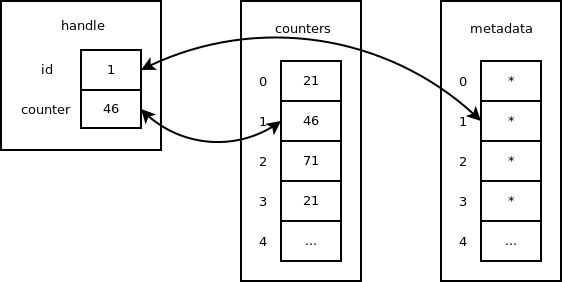
\includegraphics[width=0.80000\textwidth]{source/figures/handle.png}
\caption{ECST advanced features: accessing entity metadata through
handle}\label{handlepic}
\end{figure}

\chapter{Future work}\label{future-work}

ECST is in an experimental state and several design and implementation
choices are subject to change. This chapter aims to provide a brief
overview of the currently planned additions and adjustments.

\section{System instance
generalization}\label{system-instance-generalization}

Currently \protect\hyperlink{storage_system}{\emph{system instances}}
are closely tied to the concept of entity subscription and
unsubscription. In the future, a more general system instance class will
be introduced that will represent a \textbf{``generic computation
step''} in the depedency DAG.

Generalized system instances will have no knowledge of entities and
purely act on component data: this concept, alongside specialized
component storage strategies, will allow to easily deal with SIMD
operations.

\section{Deferred function queue}\label{deferred-function-queue}

\protect\hyperlink{flow_exec_dfuncs}{\emph{Deferred functions}} are
implemented using
\mintinline[numbersep=12pt, fontsize=\footnotesize, xleftmargin=17pt, linenos, mathescape, bgcolor=codebg]{text}{std::vector<std::function>}
in the current version of ECST, introducing unnecessary run-time
overhead due to dynamic allocation and polymorphism.

As suggested by \href{https://twitter.com/cppsage}{Matt Calabrese}, a
specialized \textbf{``deferred function queue''} class will be
introduced in the future, which will store callable objects of various
size in the same resizable buffer. This will be achieved using
fixed-size structures that will act similarly to \emph{``vtables''},
which will be stored before their corresponding callable object in the
buffer. A separate lightweight index will keep track of all the vtables
- iterating over them will allow efficient sequential execution of
deferred functions.

Appending functions to the queue will not require any additional memory
allocation.

\section{Declarative option map
interfaces}\label{declarative-option-map-interfaces}

Definining interfaces for
\protect\hyperlink{metaprogramming_option_maps}{\emph{option maps}}
requires the creation of a class and multiple methods which explicitly
need to check option value domains and update the option map. The
possibility of streamlining the definitions of compile-time option
interfaces using a declarative approach will be explored in the future -
the goal is to create a small code-generation library/module that will
generate rich compile-time option sets with an intuitive and safe user
interface.

\section{Streaming system outputs}\label{streaming-system-outputs}

Currently, a system depedendent on the output of another must wait until
its parent's execution has been completed. Sometimes outputs could be
processed as soon as they are generated connecting systems through a
\protect\hyperlink{sys_streamqueue}{\textbf{streaming queue}} - the
inclusion of this feature will be investigated in the future.

\chapter{Miscellaneous}\label{miscellaneous}

\hypertarget{appendix_sparse_integer_sets}{\section{Sparse integer
sets}\label{appendix_sparse_integer_sets}}

A \textbf{sparse integer set} is a data structures representing a set of
positive integers with the following time complexity characteristics:

\begin{longtable}[]{@{}lc@{}}
\toprule
& Time complexity\tabularnewline
\midrule
\endhead
Check presence of integer & \(\mathcal{O}(1)\)\tabularnewline
Add integer to set & \(\mathcal{O}(1)\)\tabularnewline
Remove integer from set & \(\mathcal{O}(1)\)\tabularnewline
Iterate over integers & \(\mathcal{O}(n)\)\tabularnewline
\bottomrule
\end{longtable}

Its space complexity is \(\mathcal{O}(n)\).

Sparse integers sets are perfect for entity ID management, as the
complexity of all required operations is optimal. They have been
extensively covered in {[}\protect\hyperlink{ref-sparsesets132}{30}{]}
and {[}\protect\hyperlink{ref-sparsesets_praxis}{31}{]}. A possible C++
implementation is analyzed in
{[}\protect\hyperlink{ref-sparsesets_cpp}{32}{]}. Sparse integer sets
have been already used in existing ECS libraries: an example is
\emph{Diana}, by Vincent Adam Burns
{[}\protect\hyperlink{ref-github_diana}{33}{]}.

\subsection{Implementation details}\label{implementation-details-4}

Sparse integer sets are implemented in \textbf{vrm\_core} \emph{(see
{[}\protect\hyperlink{ref-github_vrmcore}{34}{]})}, which is a
dependency of ECST. The used storage types depend on context settings
\emph{(\protect\hyperlink{appendix_static_dispatching}{static
dispatching})}, but conceptually every implementation is composed of the
following elements:

\begin{itemize}
\item
  An unordered \textbf{dense array} \(D\), which contiguously stores all
  integers present in the set;
\item
  A \textbf{sparse array} \(S\), containing indices to the elements of
  \(D\), or special null \(\emptyset\) values.
\end{itemize}

\begin{figure}[htbp]
\centering
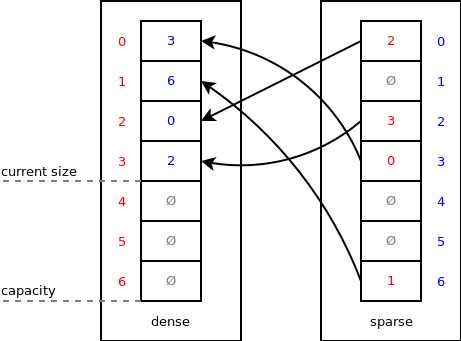
\includegraphics[width=0.85000\textwidth]{source/figures/sparseset.png}
\caption{ECST miscellaneous: fixed sparse integer set
example}\label{sparsesetexample}
\end{figure}

\subsubsection{Operation: contains}\label{operation-contains}

Checking whether or not an integer \(i\) is in the set consists in
checking if \(S_i \neq \emptyset\).

\subsubsection{Operation: iteration}\label{operation-iteration}

Iterating over the integers in the set consists in iterating over \(D\).

\subsubsection{Operation: add integer to
set}\label{operation-add-integer-to-set}

Adding an integer \(i\) to the set consists in appending it to \(D\) and
making \(S_i\) \emph{point} to \(D_{last}\).

\begin{algorithm}[H]

\caption{ECST miscellaneous: SparseIntSet - AddInteger}
\footnotesize

\SetKwData{I}{i}
\SetKwArray{D}{D}
\SetKwArray{S}{S}
\SetKwData{Last}{last}
\SetKwFunction{Contains}{Contains}

    \tcc{do nothing if \I is already in the set}
    \If{\Contains{\I} $=$ false}{
        \tcc{append \I to \D}
        \D{\Last} $\longleftarrow$ \I\;

        \tcc{make \S{\I} "point" to \I}
        \S{\I} $\longleftarrow$ \Last;
    }

\end{algorithm}

\subsubsection{Operation: remove integer from
set}\label{operation-remove-integer-from-set}

Removing an integer \(i\) from the set consists in swapping \(i\) with
\(D_{last}\) if necessary, then updating \(S_i\) and decrementing the
number of contained integers.

\begin{algorithm}[H]

\caption{ECST miscellaneous: SparseIntSet - RemoveInteger}
\footnotesize

\SetKwData{I}{i}
\SetKwData{J}{iPtr}
\SetKwArray{D}{D}
\SetKwArray{S}{S}
\SetKwData{Last}{last}
\SetKwFunction{Contains}{Contains}

    \tcc{do nothing if \I is not in the set}
    \If{\Contains{\I} $=$ true}{
        \tcc{access \S{\I}}
        \J $\longleftarrow$ \S{\I}\;

        \tcc{check if \J is the last element in \D}
        \If{\D{\Last} $\neq$ \D{\J}}{
            \tcc{if not, swap \J with the last element and update \S}
            \D{\J} $\longleftarrow$ \D{\Last}\;
            \S{\Last} $\longleftarrow$ \J\;
        }

        \tcc{nullify \S{\I} and decrement \Last}
        \S{\I} $\longleftarrow \emptyset$\;
        ${-}{-}$\Last\;
    }

\end{algorithm}

\hypertarget{appendix_component_bitset_creation}{\section{Component
bitset creation}\label{appendix_component_bitset_creation}}

\textbf{Component bitsets} are \emph{dense bitsets} implemented with
\mintinline[numbersep=12pt, fontsize=\footnotesize, xleftmargin=17pt, linenos, mathescape, bgcolor=codebg]{text}{std::bitset}
used to keep track of an entity's components and to efficiently check
whether or not an entity belongs to a system. Every component type is
represented by a unique bit.

\protect\hyperlink{storage_system}{System instances} store a component
bitset that represents the required component types for subscription.
The bitset is generated from a \protect\hyperlink{system_sigs}{system
signature}, using compile-time tuple iteration and Boost.Hana
algorithms.

Firstly, the component types specified in the system signature are
retrieved and concatenated:

\begin{minted}[numbersep=12pt, fontsize=\footnotesize, xleftmargin=17pt, linenos, mathescape]{cpp}
template <typename TSystemSignature, typename TSettings>
auto make_from_system_signature(TSystemSignature ss, TSettings s)
{
    // The "read" and "write" component tags are concatenated.
    auto all = boost::hana::concat(
        ss.read_ctag_list(), ss.write_ctag_list());

    // The complete list is passed to the `make_from_tag_list` 
    // function, which will create the bitset.
    return make_from_tag_list(s, all);
}
\end{minted}

Tags are values, and that type lists are
\mintinline[numbersep=12pt, fontsize=\footnotesize, xleftmargin=17pt, linenos, mathescape, bgcolor=codebg]{text}{boost::hana::tuple}
instances. Boost.Hana provides a
\mintinline[numbersep=12pt, fontsize=\footnotesize, xleftmargin=17pt, linenos, mathescape, bgcolor=codebg]{text}{boost::hana::for_each}
function that can be used to \emph{``iterate''} over the elements of a
tuple at compile-time. Building the bitset simply consists in iterating
over
\mintinline[numbersep=12pt, fontsize=\footnotesize, xleftmargin=17pt, linenos, mathescape, bgcolor=codebg]{text}{ctag_list}
and setting the corresponding component bits to
\mintinline[numbersep=12pt, fontsize=\footnotesize, xleftmargin=17pt, linenos, mathescape, bgcolor=codebg]{text}{1}:

\begin{minted}[numbersep=12pt, fontsize=\footnotesize, xleftmargin=17pt, linenos, mathescape]{cpp}
template <typename TSettings, typename TComponentTagList>
auto make_from_tag_list(TSettings s, TComponentTagList ctl)
{
    // Create empty `std::bitset` with length equal to the
    // number of components.
    component_bitset<TSettings> b;

    // Retrieve the complete list of component signatures
    // from the context settings.
    auto csl = settings::component_signature_list(s);

    // For each tag in `ctl`...
    boost::hana::for_each(ctl, [&](auto ct)
        {
            // Retrieve the unique component ID from `csl`.
            auto id(signature_list::component::id_by_tag(csl, ct));

            // Set the corresponding bit.
            b.set(id, true);
        });

    return b;
}
\end{minted}

\hypertarget{appendix_static_dispatching}{\section{Static
dispatching}\label{appendix_static_dispatching}}

\textbf{``Static dispatching''} is the term used in ECST to refer to
compile-time choices regarding data structures. It is used to avoid
unnecessary overhead depending on user-specified context settings. An
example use case can be found in the implementation of
\protect\hyperlink{storage_entity}{entity metadata storage}:
\mintinline[numbersep=12pt, fontsize=\footnotesize, xleftmargin=17pt, linenos, mathescape, bgcolor=codebg]{text}{std::array}
or
\mintinline[numbersep=12pt, fontsize=\footnotesize, xleftmargin=17pt, linenos, mathescape, bgcolor=codebg]{text}{std::vector}
will be used to store metadata depending on the
\emph{fixed}/\emph{dynamic} entity limit choice made by the user.

\subsection{Implementation details}\label{implementation-details-5}

Most occurrences of static dispatching are implemented using
\mintinline[numbersep=12pt, fontsize=\footnotesize, xleftmargin=17pt, linenos, mathescape, bgcolor=codebg]{text}{static_if},
available in \textbf{vrm\_core} \emph{(see
{[}\protect\hyperlink{ref-github_vrmcore}{34}{]})}. A compile-time
branching construct is not yet part of the standard, but it has been
proposed several times \emph{(see
{[}\protect\hyperlink{ref-isocpp_sif0}{35}{]},
{[}\protect\hyperlink{ref-isocpp_sif1}{36}{]},
{[}\protect\hyperlink{ref-isocpp_sif2}{37}{]} and
{[}\protect\hyperlink{ref-isocpp_sif3}{38}{]})} and it's likely to be
introduced in C++17. Nevertheless, a
\mintinline[numbersep=12pt, fontsize=\footnotesize, xleftmargin=17pt, linenos, mathescape, bgcolor=codebg]{text}{static_if}
construct that's more convienient and localized than \emph{explicit
template specialization}
{[}\protect\hyperlink{ref-cppreference_ets}{39}{]} can be implemented
using C++14 features \emph{(see {[}\protect\hyperlink{ref-sif0}{40}{]},
{[}\protect\hyperlink{ref-sif1}{41}{]} and
{[}\protect\hyperlink{ref-sif2}{42}{]})}.

Using
\mintinline[numbersep=12pt, fontsize=\footnotesize, xleftmargin=17pt, linenos, mathescape, bgcolor=codebg]{text}{static_if},
implementing static dispatching becomes straightforward. An auxiliary
\mintinline[numbersep=12pt, fontsize=\footnotesize, xleftmargin=17pt, linenos, mathescape, bgcolor=codebg]{text}{dispatch_on_storage_type}
function executes one of the passed callable objects depending on the
user-specified storage limitations:

\begin{minted}[numbersep=12pt, fontsize=\footnotesize, xleftmargin=17pt, linenos, mathescape]{cpp}
template <typename TSettings, typename TFFixed, typename TFDynamic>
auto dispatch_on_storage_type(
    TSettings&& s, TFFixed&& f_fixed, TFDynamic&& f_dynamic)
{
    return static_if(s.has_fixed_capacity())
        .then([&](auto xs)
            {
                return f_fixed(xs.get_fixed_capacity());
            })
        .else_([&](auto xs)
            {
                return f_dynamic(xs.get_dynamic_capacity());
            })(s);
}
\end{minted}

Using the function above, data structures wrapped in
\href{http://www.boost.org/doc/libs/1_61_0/libs/hana/doc/html/structboost_1_1hana_1_1type.html\#ae35139e732c4b75e91061513cf445628}{\mintinline[numbersep=12pt, fontsize=\footnotesize, xleftmargin=17pt, linenos, mathescape, bgcolor=codebg]{text}{boost::hana::type_c}}
can be returned and later instantiated. Here is the implementation of
the function statically dispatching entity metadata storage types:

\begin{minted}[numbersep=12pt, fontsize=\footnotesize, xleftmargin=17pt, linenos, mathescape]{cpp}
template <typename TSettings>
auto dispatch_entity_storage(TSettings s)
{
    return settings::dispatch_on_storage_type(s,
        [](auto fixed_capacity)
        {
            return boost::hana::type_c<
                impl::fixed_entity_storage<
                    metadata_type<TSettings>,
                    fixed_capacity>
                >;
        },
        [](auto)
        {
            return boost::hana::type_c<
                impl::dynamic_entity_storage<
                    TSettings,
                    metadata_type<TSettings>>
                >;
        });
}
\end{minted}

\hypertarget{appendix_compiletime_bfs}{\section{Compile-time
breadth-first traversal}\label{appendix_compiletime_bfs}}

A compile-time version of the \textbf{breadth-first traversal} algorithm
was implemented in order to allow users to begin system execution from
particular independent nodes. A complete
\protect\hyperlink{ctopts_siglist}{system signature list} represents a
DAG that can be composed of multiple \emph{connected components} -
knowledge of the exact number of nodes in a connected component is
required to properly execute the system chain using the
\protect\hyperlink{mt_ac_scheduler}{``atomic counter'' scheduler}.

Graph traversal algorithms provide a straightforward way of counting the
number of unique nodes in a connected component. The BFT algorithm was
chosen for this task: in short, it traverses a graph starting from a
particular node and exploring all neighbor nodes first. Explored nodes
have to be \emph{``marked''} to prevent redundant traversals.

Breadth-first traversal is easy to implement using mutable data
structures:

\begin{itemize}
\item
  A queue is used to keep track of the nodes that need to be explored;

  \begin{itemize}
  \tightlist
  \item
    Unmarked neighbors of the node currently being explored are enqueued
    for future traversal.
  \end{itemize}
\item
  Explored nodes need to be marked as \emph{``visited''} to guarantee
  each node being traversed exactly once.
\end{itemize}

Similarly to the implementation of
\protect\hyperlink{metaprogramming_option_maps}{option maps}, the
required state is implemented using immutable Boost.Hana data structures
whose operations yield a new \emph{(copy)} updated structure instead of
mutating the structure in-place.

\begin{itemize}
\item
  Nodes are compile-time numerical IDs
  \emph{(\href{http://www.boost.org/doc/libs/1_61_0/libs/hana/doc/html/structboost_1_1hana_1_1integral__constant.html}{\mintinline[numbersep=12pt, fontsize=\footnotesize, xleftmargin=17pt, linenos, mathescape, bgcolor=codebg]{text}{boost::hana::integral_constant}})};
\item
  The BFT queue is a
  \href{http://www.boost.org/doc/libs/1_61_0/libs/hana/doc/html/structboost_1_1hana_1_1tuple.html}{\mintinline[numbersep=12pt, fontsize=\footnotesize, xleftmargin=17pt, linenos, mathescape, bgcolor=codebg]{text}{boost::hana::tuple}};
\item
  Nodes are \emph{``marked as visited''} by storing their ID in a
  \href{http://www.boost.org/doc/libs/1_61_0/libs/hana/doc/html/structboost_1_1hana_1_1tuple.html}{\mintinline[numbersep=12pt, fontsize=\footnotesize, xleftmargin=17pt, linenos, mathescape, bgcolor=codebg]{text}{boost::hana::tuple}};
\item
  Both the queue and the \emph{``visited nodes tuple''} are stored in a
  \href{http://www.boost.org/doc/libs/1_61_0/libs/hana/doc/html/structboost_1_1hana_1_1pair.html}{\mintinline[numbersep=12pt, fontsize=\footnotesize, xleftmargin=17pt, linenos, mathescape, bgcolor=codebg]{text}{boost::hana::pair}}.
  The pair is referred to as the \textbf{BFT context}.
\end{itemize}

All operations are defined inside the
\mintinline[numbersep=12pt, fontsize=\footnotesize, xleftmargin=17pt, linenos, mathescape, bgcolor=codebg]{text}{bf_traversal}
namespace. The data structures can be initialized and accessed with the
following functions:

\begin{minted}[numbersep=12pt, fontsize=\footnotesize, xleftmargin=17pt, linenos, mathescape]{cpp}
namespace bf_traversal
{
    template <typename TStartNodeList>
    constexpr auto make(TStartNodeList&& snl)
    {
        return hana::make_pair(snl, hana::make_tuple());
    }

    template <typename TBFTContext>
    constexpr auto queue(TBFTContext&& c)
    {
        return hana::first(c);
    }

    template <typename TBFTContext>
    constexpr auto visited(TBFTContext&& c)
    {
        return hana::second(c);
    }
}
\end{minted}

Convenient functions to query the state of the BFT context are defined
as well:

\begin{minted}[numbersep=12pt, fontsize=\footnotesize, xleftmargin=17pt, linenos, mathescape]{cpp}
namespace bf_traversal
{
    template <typename TBFTContext, typename TNode>
    constexpr auto is_visited(TBFTContext&& c, TNode&& n)
    {
        return hana::contains(visited(c), n);
    }

    template <typename TBFTContext, typename TNode>
    constexpr auto is_in_queue(TBFTContext&& c, TNode&& n)
    {
        return hana::contains(queue(c), n);
    }

    template <typename TBFTContext>
    constexpr auto is_queue_empty(TBFTContext&& c)
    {
        return hana::is_empty(queue(c));
    }

    template <typename TBFTContext>
    constexpr auto top_node(TBFTContext&& c)
    {
        return hana::front(queue(c));
    }
}
\end{minted}

The algorithm is executed through the
\mintinline[numbersep=12pt, fontsize=\footnotesize, xleftmargin=17pt, linenos, mathescape, bgcolor=codebg]{text}{bf_traversal::execute}
function, which takes a list of starting nodes and the complete system
signature list as parameters. A
\mintinline[numbersep=12pt, fontsize=\footnotesize, xleftmargin=17pt, linenos, mathescape, bgcolor=codebg]{text}{step}
lambda, which repeatedly yields updated BFT context instances, is
executed recursively until the traversal is completed by using
\href{http://www.boost.org/doc/libs/1_61_0/libs/hana/doc/html/group__group-functional.html\#ga1393f40da2e8da6e0c12fce953e56a6c}{\mintinline[numbersep=12pt, fontsize=\footnotesize, xleftmargin=17pt, linenos, mathescape, bgcolor=codebg]{text}{boost::hana::fix}},
which is an implementation of the \textbf{``Y-combinator''}
\emph{(a.k.a. ``fixed-point combinator'')}.
\mintinline[numbersep=12pt, fontsize=\footnotesize, xleftmargin=17pt, linenos, mathescape, bgcolor=codebg]{text}{bf_traversal::execute}
returns a list of the traversed node IDs.

\begin{minted}[numbersep=12pt, fontsize=\footnotesize, xleftmargin=17pt, linenos, mathescape]{cpp}
template <typename TStartNodeList, typename TSSL>
auto execute(TStartNodeList&& snl, TSSL ssl)
{
    // Recursive step.
    // Takes itself as `self`, and the current context.
    auto step = [=](auto self, auto&& ctx)
    {
        return static_if(bf_traversal::is_queue_empty(ctx))
            .then([=](auto)
                {
                    // Base case: empty BFT queue.
                    // Return an empty tuple.
                    return hana::make_tuple();
                })
            .else_([=](auto&& x_ctx)
                {
                    // Recursive case.
                    // Call `self` with the updated context
                    // returned by `step_forward`.
                    // Append the last visited node to the
                    // final result.

                    auto updated_ctx =
                        step_forward(x_ctx, ssl);

                    return hana::append(
                        self(updated_ctx),
                        top_node(x_ctx));
                })(ctx);
    };

    // Begin the recursion vy initializing a BFT context.
    return hana::fix(step)(make(snl));
}
\end{minted}

The core of the algorithm resides in the
\mintinline[numbersep=12pt, fontsize=\footnotesize, xleftmargin=17pt, linenos, mathescape, bgcolor=codebg]{text}{bf_traversal::step_forward}
function:

\begin{minted}[numbersep=12pt, fontsize=\footnotesize, xleftmargin=17pt, linenos, mathescape]{cpp}
template <typename TBFTContext, typename TSSL>
auto step_forward(TBFTContext&& c, TSSL ssl) noexcept
{
    // Dequeue the first node.
    auto pop_queue = hana::remove_at(queue(c), mp::sz_v<0>);

    // List of neighbors of the dequeued node.
    auto neighbors = dependent_ids_list(
        ssl, signature_by_id(ssl, top_node(c)));

    // Filter out already visited neighbors.
    auto unvisited_neighbors =
        hana::remove_if(neighbors, [=](auto x_nbr)
            {
                return is_visited(c, x_nbr);
            });

    // Updated queue.
    auto new_queue =
        hana::concat(pop_queue, unvisited_neighbors);

    // Updated "visited nodes" list.
    auto new_visited =
        hana::concat(visited(c), unvisited_neighbors);

    // Updated BFT context.
    return hana::make_pair(new_queue, new_visited);
}
\end{minted}

The last missing piece is the implementation of
\mintinline[numbersep=12pt, fontsize=\footnotesize, xleftmargin=17pt, linenos, mathescape, bgcolor=codebg]{text}{dependent_ids_list},
which returns a list of nodes that depend on the passed \emph{``parent
node''}. It is implemented by iterating over the complete system
signature list \emph{(using
\href{http://www.boost.org/doc/libs/1_61_0/libs/hana/doc/html/fold__right_8hpp.html}{\mintinline[numbersep=12pt, fontsize=\footnotesize, xleftmargin=17pt, linenos, mathescape, bgcolor=codebg]{text}{boost::hana::fold_right}})},
gathering all nodes that have the \emph{``parent node''} as one of their
dependencies:

\begin{minted}[numbersep=12pt, fontsize=\footnotesize, xleftmargin=17pt, linenos, mathescape]{cpp}
template <typename TSystemSignatureList, typename TSystemSignature>
auto dependent_ids_list(
    TSystemSignatureList ssl, TSystemSignature parent)
{
    namespace ss = signature::system;
    namespace sls = signature_list::system;

    // Retrieve the id of `parent`.
    auto parent_id = sls::id_by_signature(ssl, parent);

    // Build a list of dependent IDs.
    return hana::fold_right(ssl, hana::make_tuple(),
        [=](auto ss, auto acc)
        {
            // Check if `parent_id` is one of `ss`'s depedendencies.
            auto dl = sls::dependencies_as_id_list(ssl, ss);
            return static_if(hana::contains(dl, parent_id))
                .then([=](auto x_acc)
                    {
                        // If so, add `ss`'s ID to the result list.
                        auto ss_id = sls::id_by_signature(ssl, ss);
                        return hana::append(x_acc, ss_id);
                    })
                .else_([=](auto x_acc)
                    {
                        return x_acc;
                    })(acc);
        });
}
\end{minted}

\protect\hyperlink{mt_s_sce}{The algorithm is used in the implementation
of the
\mintinline[numbersep=12pt, fontsize=\footnotesize, xleftmargin=17pt, linenos, mathescape, bgcolor=codebg]{text}{atomic_counter::execute}
scheduler function}, under the name
\mintinline[numbersep=12pt, fontsize=\footnotesize, xleftmargin=17pt, linenos, mathescape, bgcolor=codebg]{text}{chain_size},
in order to instantiate a
\mintinline[numbersep=12pt, fontsize=\footnotesize, xleftmargin=17pt, linenos, mathescape, bgcolor=codebg]{text}{counter_blocker}
that will block the calling thread until all systems belonging to a
particular connected component of the dependency DAG have been executed.

\part{Example ECST applications and benchmarks}

\hypertarget{part3_sim}{\chapter{Overview}\label{part3_sim}}

In this part two simple applications implemented using ECST will be
analyzed, in order to provide the readers with usage examples of the
library and with performance comparisons between various combinations of
the compile-time multithreading options:

\begin{itemize}
\item
  A \textbf{2D real-time particle simulation}, where circular particles
  collide with each other in a closed space;
\item
  A \textbf{real-time entity creation/destruction benchmark}, where
  entities with a limited life replicate themselves a fixed amout of
  times.
\end{itemize}

\chapter{2D particle simulation}\label{d-particle-simulation}

\section{Description}\label{description}

The simulation consists in a number of \textbf{rigid-body circular
particles} of various radius, colliding with each other in a closed
space. The particle entities are generated at the beginning of the demo.
A \textbf{2D grid} spatial partitioning system is used to speed-up
broadphase collision detection. Every particle has a \textbf{life} timer
that constantly gets decremented: the entity is destroyed as soon as the
timer reaches zero. When all the particles are destroyed, the simulation
automatically ends.

Multiple simulations are executed and benchmarked, combining the
following compile-time options and parameters:

\begin{itemize}
\item
  Entity count: \(50000\), \(100000\) and \(200000\);
\item
  Inner parallelism: \textbf{enabled} or \textbf{disabled};
\item
  Entity storage strategy: \textbf{fixed} or \textbf{dynamic}.
\end{itemize}

In total, \(12\) simulations are executed.

The \href{http://sfml-dev.org}{SFML} library is used for rendering and
math utilities.

\section{Components}\label{components}

Every particle is composed of the following component types:

\begin{itemize}
\item
  \textbf{Position}: 2D
  \mintinline[numbersep=12pt, fontsize=\footnotesize, xleftmargin=17pt, linenos, mathescape, bgcolor=codebg]{text}{float}
  vector;

  \begin{minted}[numbersep=12pt, fontsize=\footnotesize, xleftmargin=17pt, linenos, mathescape]{cpp}
  struct position { sf::Vector2f _v; };
  \end{minted}
\item
  \textbf{Velocity}: 2D
  \mintinline[numbersep=12pt, fontsize=\footnotesize, xleftmargin=17pt, linenos, mathescape, bgcolor=codebg]{text}{float}
  vector;

  \begin{minted}[numbersep=12pt, fontsize=\footnotesize, xleftmargin=17pt, linenos, mathescape]{cpp}
  struct velocity { sf::Vector2f _v; };
  \end{minted}
\item
  \textbf{Acceleration}: 2D
  \mintinline[numbersep=12pt, fontsize=\footnotesize, xleftmargin=17pt, linenos, mathescape, bgcolor=codebg]{text}{float}
  vector;

  \begin{minted}[numbersep=12pt, fontsize=\footnotesize, xleftmargin=17pt, linenos, mathescape]{cpp}
  struct acceleration { sf::Vector2f _v; };
  \end{minted}
\item
  \textbf{Color}: used for SFML rendering;

  \begin{minted}[numbersep=12pt, fontsize=\footnotesize, xleftmargin=17pt, linenos, mathescape]{cpp}
  struct color { sf::Color _v; };
  \end{minted}
\item
  \textbf{Circle}: shape of the particle, controls its radius;

  \begin{minted}[numbersep=12pt, fontsize=\footnotesize, xleftmargin=17pt, linenos, mathescape]{cpp}
  struct circle { float _radius; };
  \end{minted}
\item
  \textbf{Life}: controls the lifetime of a particle.

  \begin{minted}[numbersep=12pt, fontsize=\footnotesize, xleftmargin=17pt, linenos, mathescape]{cpp}
  struct life { float _v; };
  \end{minted}
\end{itemize}

\section{Systems}\label{systems}

\begin{itemize}
\item
  \textbf{Acceleration}: increments each particle's
  \mintinline[numbersep=12pt, fontsize=\footnotesize, xleftmargin=17pt, linenos, mathescape, bgcolor=codebg]{text}{velocity}
  vector by its
  \mintinline[numbersep=12pt, fontsize=\footnotesize, xleftmargin=17pt, linenos, mathescape, bgcolor=codebg]{text}{acceleration}
  vector;

  \begin{itemize}
  \tightlist
  \item
    Multithreading is enabled.
  \end{itemize}
\item
  \textbf{Velocity}: increments each particle's
  \mintinline[numbersep=12pt, fontsize=\footnotesize, xleftmargin=17pt, linenos, mathescape, bgcolor=codebg]{text}{position}
  vector by its
  \mintinline[numbersep=12pt, fontsize=\footnotesize, xleftmargin=17pt, linenos, mathescape, bgcolor=codebg]{text}{velocity}
  vector;

  \begin{itemize}
  \tightlist
  \item
    Multithreading is enabled.
  \end{itemize}
\item
  \textbf{Keep in bounds}: keeps every particle inside the boundaries of
  the simulation;

  \begin{itemize}
  \tightlist
  \item
    Multithreading is enabled.
  \end{itemize}
\item
  \textbf{Spatial partition}: stores the 2D spatial partitioning grid
  and manages it;

  \begin{itemize}
  \item
    Multithreading is enabled;
  \item
    Produces
    \mintinline[numbersep=12pt, fontsize=\footnotesize, xleftmargin=17pt, linenos, mathescape, bgcolor=codebg]{text}{std::vector<sp_data>}
    outputs.
    \mintinline[numbersep=12pt, fontsize=\footnotesize, xleftmargin=17pt, linenos, mathescape, bgcolor=codebg]{text}{sp_data}
    is a lightweight
    \mintinline[numbersep=12pt, fontsize=\footnotesize, xleftmargin=17pt, linenos, mathescape, bgcolor=codebg]{text}{struct}
    holding an
    \mintinline[numbersep=12pt, fontsize=\footnotesize, xleftmargin=17pt, linenos, mathescape, bgcolor=codebg]{text}{entity_id}
    and a pair of 2D cells coordinates. The produced vectors will be
    read from the context step in order to fill the stored 2D grid data
    structure.
  \end{itemize}
\item
  \textbf{Collision detection}: detects collisions between particles
  \emph{(filtered by the broadphase spartial partitioning system)}. The
  detected collisions are resolved by a subsequent system;

  \begin{itemize}
  \item
    Multithreading is enabled;
  \item
    Produces
    \mintinline[numbersep=12pt, fontsize=\footnotesize, xleftmargin=17pt, linenos, mathescape, bgcolor=codebg]{text}{std::vector<contact>}
    outputs.
    \mintinline[numbersep=12pt, fontsize=\footnotesize, xleftmargin=17pt, linenos, mathescape, bgcolor=codebg]{text}{contact}
    is a lightweight
    \mintinline[numbersep=12pt, fontsize=\footnotesize, xleftmargin=17pt, linenos, mathescape, bgcolor=codebg]{text}{struct}
    holding
    \mintinline[numbersep=12pt, fontsize=\footnotesize, xleftmargin=17pt, linenos, mathescape, bgcolor=codebg]{text}{entity_id}
    instances of two colliding particles. The contacts sequentially read
    from the
    \mintinline[numbersep=12pt, fontsize=\footnotesize, xleftmargin=17pt, linenos, mathescape, bgcolor=codebg]{text}{solve_contacts}
    system to solve penetration between particles.
  \end{itemize}
\item
  \textbf{Solve contacts}: reads
  \mintinline[numbersep=12pt, fontsize=\footnotesize, xleftmargin=17pt, linenos, mathescape, bgcolor=codebg]{text}{collision}'s
  produced
  \mintinline[numbersep=12pt, fontsize=\footnotesize, xleftmargin=17pt, linenos, mathescape, bgcolor=codebg]{text}{contact}
  outputs and sequentially solves penetration between particles;

  \begin{itemize}
  \tightlist
  \item
    Multithreading is disabled.
  \end{itemize}
\item
  \textbf{Render colored circle}: deals with particle rendering;

  \begin{itemize}
  \item
    Multithreading is enabled;
  \item
    Produces
    \mintinline[numbersep=12pt, fontsize=\footnotesize, xleftmargin=17pt, linenos, mathescape, bgcolor=codebg]{text}{std::vector<sf::Vertex>}
    outputs. The vertices are used to render the circles using SFML.
  \end{itemize}
\item
  \textbf{Life}: deals with particle lifetime. Continuously decreases
  every particle's
  \mintinline[numbersep=12pt, fontsize=\footnotesize, xleftmargin=17pt, linenos, mathescape, bgcolor=codebg]{text}{life}
  value and marks particles as dead when their lifetime is over;

  \begin{itemize}
  \tightlist
  \item
    Multithreading is enabled.
  \end{itemize}
\item
  \textbf{Fade}: changes particles' opacity depending on their life.

  \begin{itemize}
  \tightlist
  \item
    Multithreading is enabled.
  \end{itemize}
\end{itemize}

The implicitly generated depedency DAG is shown below:

\begin{figure}[htbp]
\centering
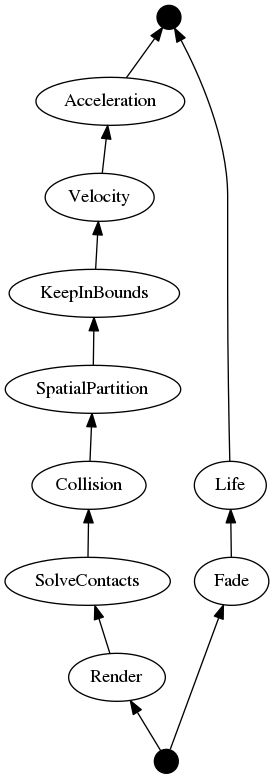
\includegraphics[height=0.85000\textwidth]{source/figures/generated/sim/dag0.png}
\caption{Particle simulation: dependency DAG}
\end{figure}

\subsection{System implementations}\label{system-implementations}

Most of the system implementations are straightforward:
\mintinline[numbersep=12pt, fontsize=\footnotesize, xleftmargin=17pt, linenos, mathescape, bgcolor=codebg]{text}{s::acceleration}
and
\mintinline[numbersep=12pt, fontsize=\footnotesize, xleftmargin=17pt, linenos, mathescape, bgcolor=codebg]{text}{s::velocity}
simply iterate over their subscribed entities, mutating the values of
the targeted components. Here is the implementation of
\mintinline[numbersep=12pt, fontsize=\footnotesize, xleftmargin=17pt, linenos, mathescape, bgcolor=codebg]{text}{s::acceleration}:

\begin{minted}[numbersep=12pt, fontsize=\footnotesize, xleftmargin=17pt, linenos, mathescape]{cpp}
struct acceleration
{
    template <typename TData>
    void process(ft dt, TData& data)
    {
        data.for_entities([&](auto eid)
            {
                auto& v = data.get(ct::velocity, eid)._v;
                const auto& a = data.get(ct::acceleration, eid)._v;
                v += a * dt;
            });
    }
};
\end{minted}

\mintinline[numbersep=12pt, fontsize=\footnotesize, xleftmargin=17pt, linenos, mathescape, bgcolor=codebg]{text}{s::fade},
\mintinline[numbersep=12pt, fontsize=\footnotesize, xleftmargin=17pt, linenos, mathescape, bgcolor=codebg]{text}{s::life}
and
\mintinline[numbersep=12pt, fontsize=\footnotesize, xleftmargin=17pt, linenos, mathescape, bgcolor=codebg]{text}{s::keep_in_bounds}
are implemented in a similar way.

\subsubsection{Spatial partition}\label{spatial-partition}

\mintinline[numbersep=12pt, fontsize=\footnotesize, xleftmargin=17pt, linenos, mathescape, bgcolor=codebg]{text}{s::spatial_parititon}
is a stateful system: it stores a 2D grid used to speed-up broadphase
collisions and produces outputs later read in \emph{step stage} to
mutate the stored grid.

The grid is implemented with two nested
\mintinline[numbersep=12pt, fontsize=\footnotesize, xleftmargin=17pt, linenos, mathescape, bgcolor=codebg]{text}{std::array}
of
\mintinline[numbersep=12pt, fontsize=\footnotesize, xleftmargin=17pt, linenos, mathescape, bgcolor=codebg]{text}{std::vector<entity_id>}:

\begin{minted}[numbersep=12pt, fontsize=\footnotesize, xleftmargin=17pt, linenos, mathescape]{cpp}
struct spatial_partition
{
    using cell_type = std::vector<ecst::entity_id>;
    std::array<std::array<cell_type, grid_height>, grid_width> _grid;
    // ...
\end{minted}

At the beginning of every step stage
\mintinline[numbersep=12pt, fontsize=\footnotesize, xleftmargin=17pt, linenos, mathescape, bgcolor=codebg]{text}{_grid}
is cleared. The
\mintinline[numbersep=12pt, fontsize=\footnotesize, xleftmargin=17pt, linenos, mathescape, bgcolor=codebg]{text}{process}
method of the system iterates over the subscribed entities and produces
\mintinline[numbersep=12pt, fontsize=\footnotesize, xleftmargin=17pt, linenos, mathescape, bgcolor=codebg]{text}{sp_data}
instances:

\begin{minted}[numbersep=12pt, fontsize=\footnotesize, xleftmargin=17pt, linenos, mathescape]{cpp}
template <typename TData>
void process(TData& data)
{
    // Get a reference to the output vector and clear it.
    auto& o = data.output();
    o.clear();

    // For every entity in the subtask...
    data.for_entities([&](auto eid)
        {
            // Access component data.
            const auto& p = data.get(ct::position, eid)._v;
            const auto& c = data.get(ct::circle, eid)._radius;

            // Figure out the broadphase cell and emplace an
            // `sp_data` instance in the output vector.
            this->for_cells_of(p, c, [eid, &o](auto cx, auto cy)
                {
                    o.emplace_back(eid, cx, cy);
                });
        });
}
\end{minted}

The
\mintinline[numbersep=12pt, fontsize=\footnotesize, xleftmargin=17pt, linenos, mathescape, bgcolor=codebg]{text}{sp_data}
struct is defined as follows:

\begin{minted}[numbersep=12pt, fontsize=\footnotesize, xleftmargin=17pt, linenos, mathescape]{cpp}
struct sp_data
{
    ecst::entity_id _e;
    sz_t _cell_x, _cell_y;
};
\end{minted}

Every subtask of
\mintinline[numbersep=12pt, fontsize=\footnotesize, xleftmargin=17pt, linenos, mathescape, bgcolor=codebg]{text}{s::spatial_partition}
will produce
\mintinline[numbersep=12pt, fontsize=\footnotesize, xleftmargin=17pt, linenos, mathescape, bgcolor=codebg]{text}{sp_data}
instances in parallel. They will be sequentially read in the step stage
to fill the 2D grid:

\begin{minted}[numbersep=12pt, fontsize=\footnotesize, xleftmargin=17pt, linenos, mathescape]{cpp}
sea::t(st::spatial_partition).detailed_instance(
    [&proxy](auto& instance, auto& executor)
    {
        // Clear 2D grid.
        auto& s(instance.system());
        s.clear_cells();

        // Produce `sp_data` instances in parallel.
        executor.for_subtasks([&s](auto& data)
            {
                s.process(data);
            });

        // Fill 2D grid sequentially.
        instance.for_outputs(
            [](auto& xs, auto& sp_vector)
            {
                for(const auto& x : sp_vector)
                {
                    xs.add_sp(x);
                }
            });
    }));
\end{minted}

\subsubsection{Collision}\label{collision}

The
\mintinline[numbersep=12pt, fontsize=\footnotesize, xleftmargin=17pt, linenos, mathescape, bgcolor=codebg]{text}{s::collision}
system will iterate over unique pairs of particles in the same spatial
partitioning cell and produce
\mintinline[numbersep=12pt, fontsize=\footnotesize, xleftmargin=17pt, linenos, mathescape, bgcolor=codebg]{text}{contact}
instances in parallel that will be sequentially processed by the
\mintinline[numbersep=12pt, fontsize=\footnotesize, xleftmargin=17pt, linenos, mathescape, bgcolor=codebg]{text}{s::solve_contacts}
system.

The
\mintinline[numbersep=12pt, fontsize=\footnotesize, xleftmargin=17pt, linenos, mathescape, bgcolor=codebg]{text}{contact}
struct is defined as follows:

\begin{minted}[numbersep=12pt, fontsize=\footnotesize, xleftmargin=17pt, linenos, mathescape]{cpp}
struct contact
{
    // IDs of the colliding entities.
    ecst::entity_id _e0, _e1;

    // Distance between entities.
    float _dist;
};
\end{minted}

As
\mintinline[numbersep=12pt, fontsize=\footnotesize, xleftmargin=17pt, linenos, mathescape, bgcolor=codebg]{text}{s::spatial_parititon}
is a dependency of
\mintinline[numbersep=12pt, fontsize=\footnotesize, xleftmargin=17pt, linenos, mathescape, bgcolor=codebg]{text}{s::collision},
its state can be safely accessed in
\mintinline[numbersep=12pt, fontsize=\footnotesize, xleftmargin=17pt, linenos, mathescape, bgcolor=codebg]{text}{s::collision::process}:

\begin{minted}[numbersep=12pt, fontsize=\footnotesize, xleftmargin=17pt, linenos, mathescape]{cpp}
template <typename TData>
void process(TData& data)
{
    // Get a reference to the output vector and clear it.
    auto& out = data.output();
    out.clear();

    // Get a reference to the `spatial_partition` system.
    auto& sp = data.system(st::spatial_partition);

    // For every entity in the subtask...
    data.for_entities([&](auto eid)
        {
            // Access the grid cell containing position `p0`.
            auto& p0 = data.get(ct::position, eid)._v;
            auto& cell = sp.cell_by_pos(p0);

            for_unique_pairs(cell, eid, [&](auto eid2)
                {
                    // Check "circle vs circle" collision
                    // and eventually emplace a `contact`
                    // instance in `out`.
                });
        });
}
\end{minted}

\section{Results}\label{results}

\subsection{Screenshots}\label{screenshots}

Two screenshots of the particle simulations are shown below. The first
one shows 50000 particle entities colliding in a closed space:

\begin{figure}[htbp]
\centering

\includegraphics{source/figures/bench/sc0.png}
\caption{Particle simulation: screenshot - 50000 colliding particles}
\end{figure}

The second one shows one of the cells of the spatial partitioning 2D
grid - all particles belonging to the cell are highlighted:

\begin{figure}[htbp]
\centering
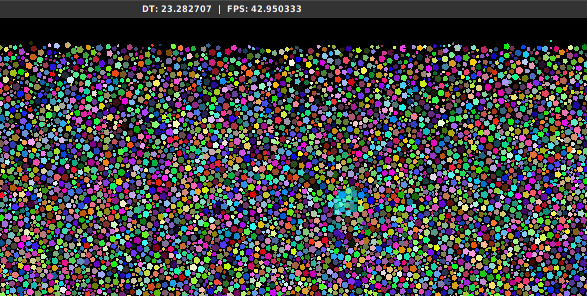
\includegraphics{source/figures/bench/sc1.png}
\caption{Particle simulation: screenshot - spatial partitioning cell}
\end{figure}

\hypertarget{bench_particlesim}{\subsection{Benchmarks}\label{bench_particlesim}}

The computer used to benchmark the particle simulation has the following
hardware specifications:

\begin{itemize}
\item
  CPU:
  \href{http://ark.intel.com/products/61275/Intel-Core-i7-2700K-Processor-8M-Cache-up-to-3_90-GHz}{\textbf{Intel®
  Core™ i7-2700K Processor} \emph{(8M Cache, up to 3.90 GHz)}};
\item
  RAM: \href{http://www.hyperxgaming.com/us/memory/beast}{\textbf{HyperX
  Beast 16GB DDR3-2400MHz}};
\item
  Motherboard:
  \href{http://www.asrock.com/mb/intel/z77\%20extreme4-m/}{\textbf{ASRock
  Z77 Extreme4-M}}.
\end{itemize}

The simulation was executed on a system with
\href{https://www.archlinux.org/}{\textbf{Arch Linux x64}} as its
operating system, using \(8\) worker threads. Rendering was disabled for
the benchmarks.

\mintinline[numbersep=12pt, fontsize=\footnotesize, xleftmargin=17pt, linenos, mathescape, bgcolor=codebg]{text}{g++}
version 6.1.1 was used, with the following compiler flags:\\
\mintinline[numbersep=12pt, fontsize=\footnotesize, xleftmargin=17pt, linenos, mathescape, bgcolor=codebg]{text}{-Ofast -march=native -ffast-math -ftree-vectorize}.

The error bars in the following graphs represent the \emph{standard
deviation}.

\subsubsection{Dynamic versus fixed entity
storage}\label{dynamic-versus-fixed-entity-storage}

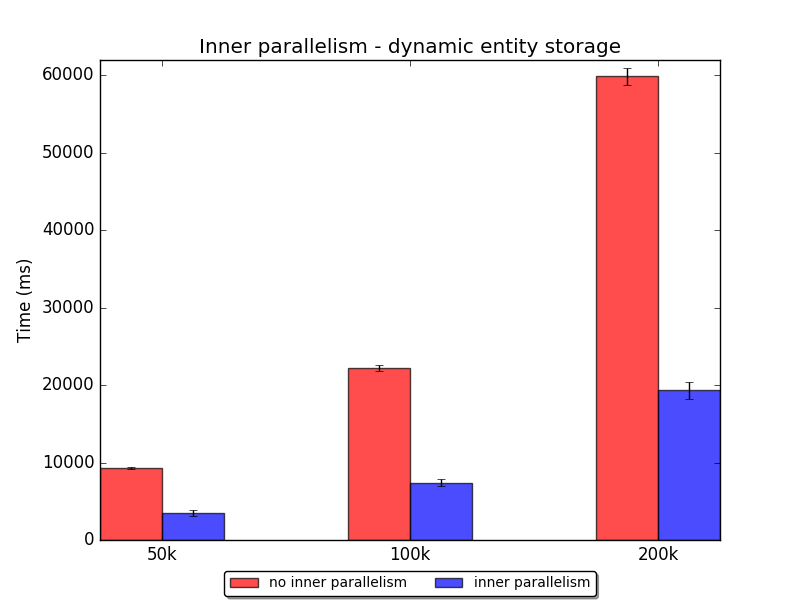
\includegraphics{source/figures/bench/ipcomp_dynamic.png}
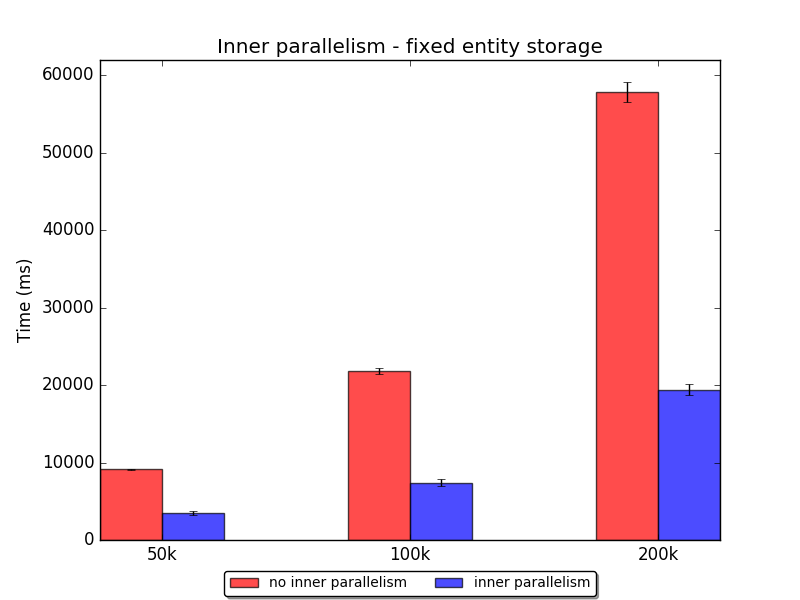
\includegraphics{source/figures/bench/ipcomp_fixed.png}

\subsubsection{Entity scaling}\label{entity-scaling}

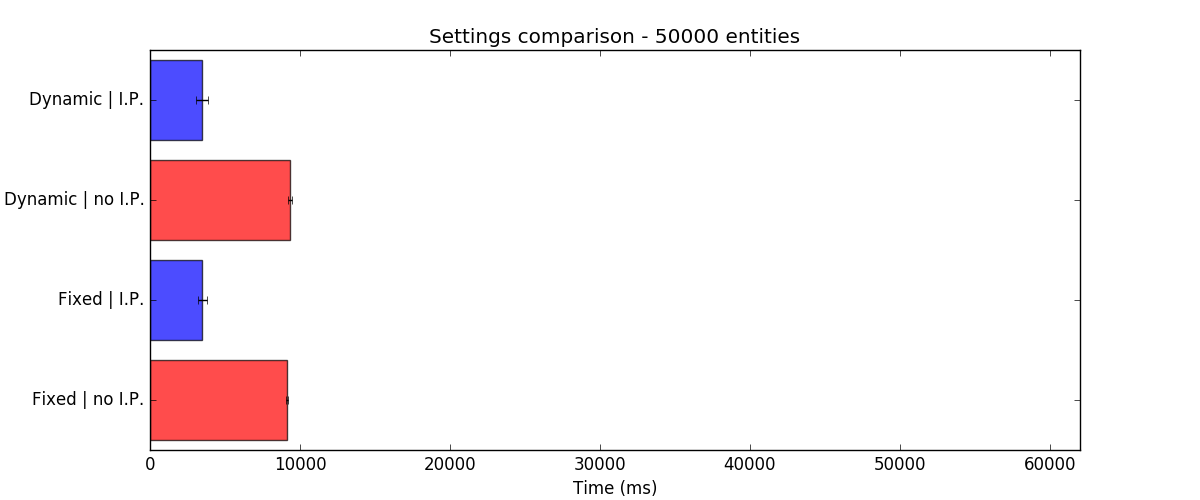
\includegraphics{source/figures/bench/entity_50k.png}
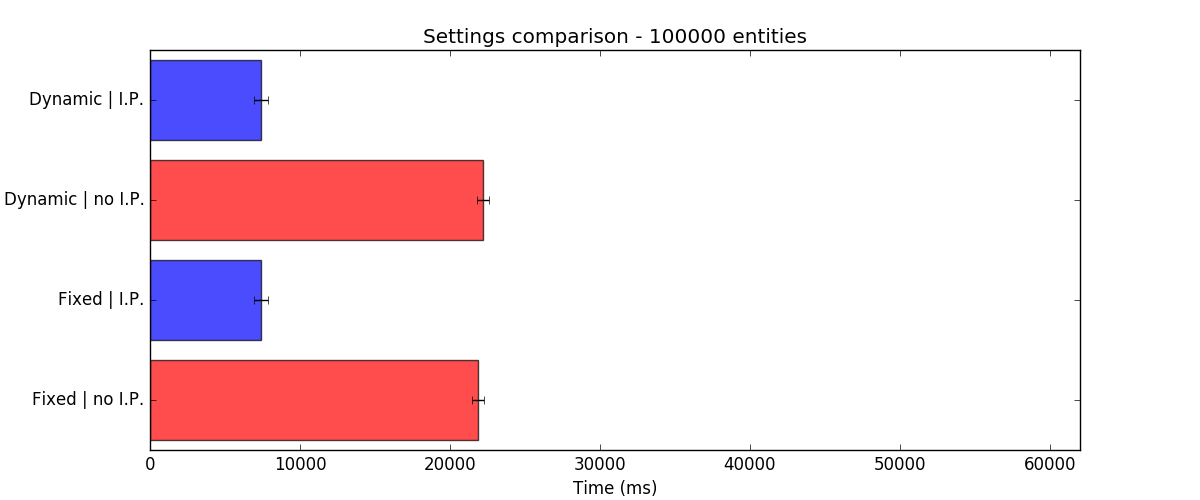
\includegraphics{source/figures/bench/entity_100k.png}
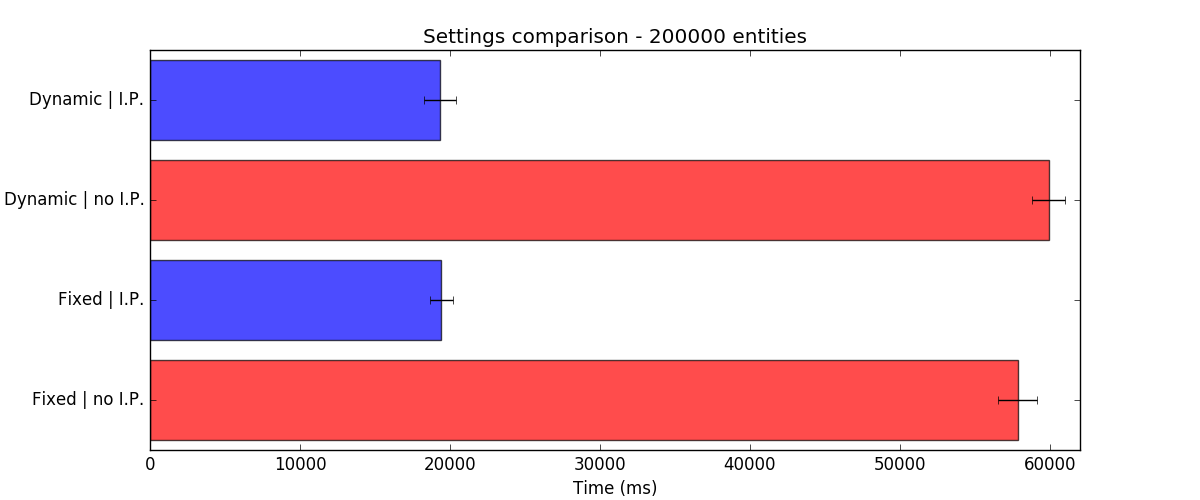
\includegraphics{source/figures/bench/entity_200k.png}

\hypertarget{bench_parsim_conc}{\section{Conclusions}\label{bench_parsim_conc}}

The following conclusions can be deduced from the benchmark graphs:

\begin{itemize}
\item
  \textbf{Fixed} entity storage seems slightly faster than
  \textbf{dynamic} entity storage when inner parallelism is disabled,
  possibly due to the fact that checks for possible reallocations during
  entity creations are not present. However, dynamic entity storage
  seems slightly faster than fixed entity storage when inner parallelism
  is enabled, even if entity creation only occurs sequentially at the
  beginning of the simulation. The results on \textbf{fixed versus
  dynamic} entity storage are therefore inconclusive with this benchmark
  - a different simulation, where entities are continuously created and
  destroyed over time, may compare the two entity storage strategies
  more fairly. The tables below shows the execution time percent change
  of the dynamic storage strategy:

  \begin{longtable}[]{@{}lll@{}}
  \toprule
  & Fixed (no I.P.) & Dynamic (no I.P.)\tabularnewline
  \midrule
  \endhead
  50k & baseline & +2.28\%\tabularnewline
  100k & baseline & +1.42\%\tabularnewline
  200k & baseline & +3.56\%\tabularnewline
  \bottomrule
  \end{longtable}

  \begin{longtable}[]{@{}lll@{}}
  \toprule
  & Fixed (I.P.) & Dynamic (I.P.)\tabularnewline
  \midrule
  \endhead
  50k & baseline & -0.45\%\tabularnewline
  100k & baseline & -0.26\%\tabularnewline
  200k & baseline & -0.44\%\tabularnewline
  \bottomrule
  \end{longtable}
\item
  As expected, splitting system execution in multiple subtasks using
  \protect\hyperlink{multithreading_inner_par}{\textbf{inner
  parallelism}} results in a huge run-time performance boost. On the
  machine used for the benchmarks, an average \(65\)\% relative
  performance increment is achieved:

  \begin{longtable}[]{@{}lcc@{}}
  \toprule
  & No inner parallelism & Inner parallelism\tabularnewline
  \midrule
  \endhead
  50k & baseline & -62.32\%\tabularnewline
  100k & baseline & -66.38\%\tabularnewline
  200k & baseline & -67.07\%\tabularnewline
  \bottomrule
  \end{longtable}
\end{itemize}

The complete source code of the example particle simulation can be found
in the following GitHub repository, under the \emph{Academic Free
License (``AFL'') v. 3.0}:
\url{https://github.com/SuperV1234/bcs_thesis}.

\chapter{Entity creation/destruction
benchmark}\label{entity-creationdestruction-benchmark}

\section{Description}\label{description-1}

The benchmark aims to measure the performance of continuous real-time
entity creation/destruction with various combinations of compile-time
settings. At the beginning of the application, a fixed number of
entities is created. The entities possess a
\mintinline[numbersep=12pt, fontsize=\footnotesize, xleftmargin=17pt, linenos, mathescape, bgcolor=codebg]{text}{c::life}
component that will destroy them after a random amount of time, creating
a new entity instance on destruction. The entity replication process is
limited by a counter stored in
\mintinline[numbersep=12pt, fontsize=\footnotesize, xleftmargin=17pt, linenos, mathescape, bgcolor=codebg]{text}{c::life}
that is decreased on creation.

As with the previous example application, multiple simulations are
executed and benchmarked, combining the following compile-time options
and parameters:

\begin{itemize}
\item
  Entity count: \(50000\), \(100000\) and \(200000\);
\item
  Inner parallelism: \textbf{enabled} or \textbf{disabled};
\item
  Entity storage strategy: \textbf{fixed} or \textbf{dynamic}.
\end{itemize}

In total, \(12\) simulations are executed.

\section{Components}\label{components-1}

The only existing component type is
\mintinline[numbersep=12pt, fontsize=\footnotesize, xleftmargin=17pt, linenos, mathescape, bgcolor=codebg]{text}{c::life}.

\begin{itemize}
\item
  \textbf{Life}: controls the lifetime of an entity and its amount of
  replications.

  \begin{minted}[numbersep=12pt, fontsize=\footnotesize, xleftmargin=17pt, linenos, mathescape]{cpp}
  struct life
  {
      float _v;
      int _spawns;
  };
  \end{minted}
\end{itemize}

\section{Systems}\label{systems-1}

\begin{itemize}
\item
  \textbf{Life}: deals with entity lifetime and replication.
  Continuously decreases every particle's
  \mintinline[numbersep=12pt, fontsize=\footnotesize, xleftmargin=17pt, linenos, mathescape, bgcolor=codebg]{text}{life}
  value and marks particles as dead when their lifetime is over. Once an
  entity is marked as dead, a
  \protect\hyperlink{flow_exec_dfuncs}{\textbf{deferred function}} that
  creates a new particle is enqueued if
  \mintinline[numbersep=12pt, fontsize=\footnotesize, xleftmargin=17pt, linenos, mathescape, bgcolor=codebg]{text}{c::life::_spawns}
  is greater than \(0\).

  \begin{itemize}
  \tightlist
  \item
    Multithreading is enabled.
  \end{itemize}
\end{itemize}

\subsection{System implementations}\label{system-implementations-1}

The commented implementation of the
\mintinline[numbersep=12pt, fontsize=\footnotesize, xleftmargin=17pt, linenos, mathescape, bgcolor=codebg]{text}{s::life}
system is provided below:

\begin{minted}[numbersep=12pt, fontsize=\footnotesize, xleftmargin=17pt, linenos, mathescape]{cpp}
struct life
{
    template <typename TData>
    void process(ft dt, TData& data)
    {
        data.for_entities([&](auto eid)
            {
                // Alias the entity's lifetime value.
                auto& l = data.get(ct::life, eid)._v;

                // Alias the entity's left replications value.
                auto& spawns = data.get(ct::life, eid)._spawns;

                // Decrease the entity's lifetime.
                l -= 10.f * dt;

                // If the lifetime value reaches zero...
                if(l <= 0.f)
                {
                    // ...mark the entity as dead.
                    data.kill_entity(eid);

                    // If the entity can replicate itself...
                    if(spawns > 0)
                    {
                        // ...enqueue a deferred function creating
                        // a new entity with one less replication.
                        data.defer([spawns](auto& proxy)
                            {
                                mk_particle(proxy, spawns - 1);
                            });
                    }
                }
            });
    }
};
\end{minted}

\section{Results}\label{results-1}

\subsection{Benchmarks}\label{benchmarks}

The \protect\hyperlink{bench_particlesim}{previously described machine
and environment} were used for this simulation.

Again, the error bars in the following graphs represent the
\emph{standard deviation}.

\subsubsection{Dynamic versus fixed entity
storage}\label{dynamic-versus-fixed-entity-storage-1}

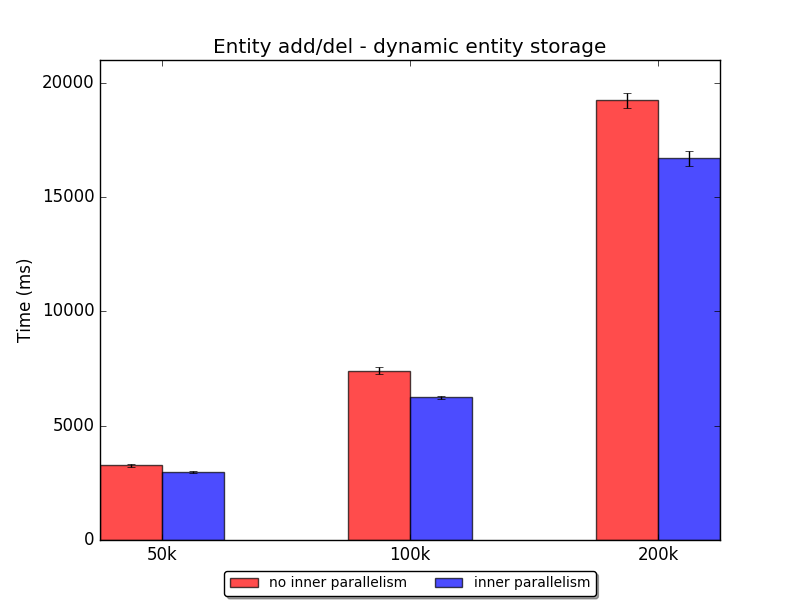
\includegraphics{source/figures/bench2/ipcomp_dynamic.png}
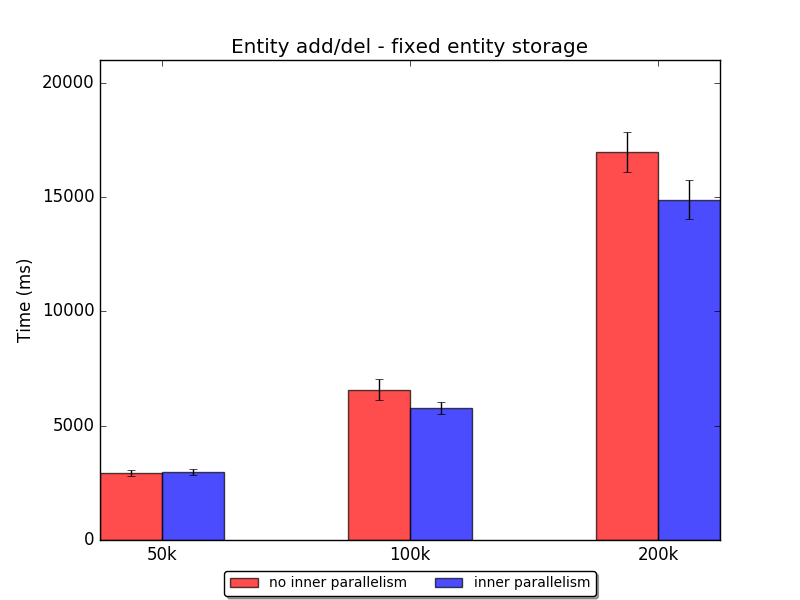
\includegraphics{source/figures/bench2/ipcomp_fixed.png}

\subsubsection{Entity scaling}\label{entity-scaling-1}

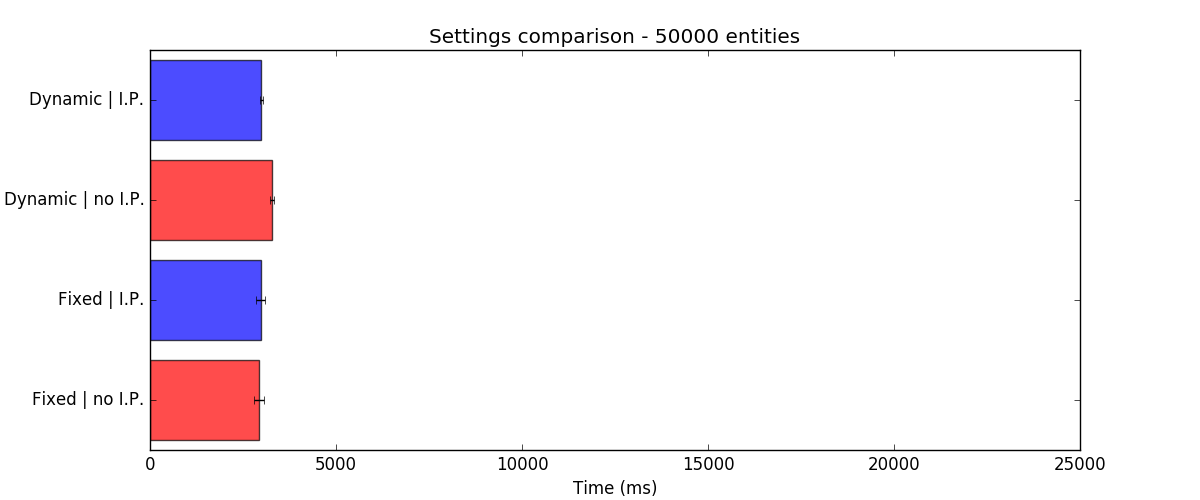
\includegraphics{source/figures/bench2/entity_50k.png}
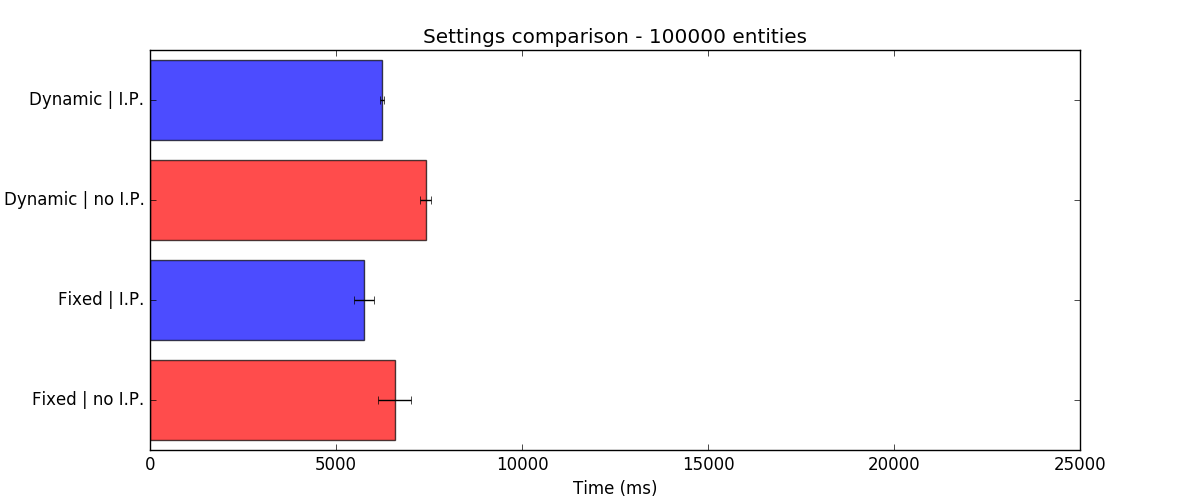
\includegraphics{source/figures/bench2/entity_100k.png}
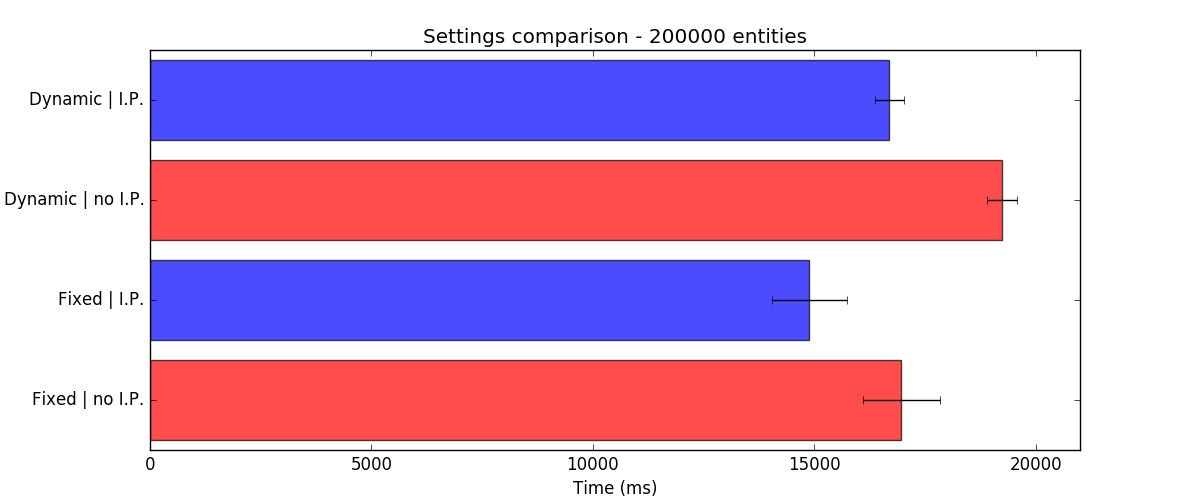
\includegraphics{source/figures/bench2/entity_200k.png}

\section{Conclusions}\label{conclusions}

The following conclusions can be deduced from the benchmark graphs:

\begin{itemize}
\item
  \textbf{Fixed} entity storage is definitely slightly faster than
  \textbf{dynamic} entity storage, indepedently of inner parallelism
  settings. The presence of reallocation checks \emph{(in dynamic entity
  storage)} produces a noticeable run-time overhead due to the huge
  number of entity creations/destructions. The tables below shows the
  execution time percent change of the dynamic storage strategy:

  \begin{longtable}[]{@{}lll@{}}
  \toprule
  & Fixed (no I.P.) & Dynamic (no I.P.)\tabularnewline
  \midrule
  \endhead
  50k & baseline & +11.77\%\tabularnewline
  100k & baseline & +12.56\%\tabularnewline
  200k & baseline & +13.34\%\tabularnewline
  \bottomrule
  \end{longtable}

  \begin{longtable}[]{@{}lll@{}}
  \toprule
  & Fixed (I.P.) & Dynamic (I.P.)\tabularnewline
  \midrule
  \endhead
  50k & baseline & +0.47\%\tabularnewline
  100k & baseline & +8.19\%\tabularnewline
  200k & baseline & +12.09\%\tabularnewline
  \bottomrule
  \end{longtable}
\item
  Again, using
  \protect\hyperlink{multithreading_inner_par}{\textbf{inner
  parallelism}} results in an expected run-time performance boost. Due
  to the nature of this simulation, however, only an average \(10\)\%
  relative performance increment is achieved compared to the
  \protect\hyperlink{bench_parsim_conc}{previous simulation's} \(65\)\%
  relative performance increment:

  \begin{longtable}[]{@{}lcc@{}}
  \toprule
  & No inner parallelism & Inner parallelism\tabularnewline
  \midrule
  \endhead
  50k & baseline & -3.98\%\tabularnewline
  100k & baseline & -14.23\%\tabularnewline
  200k & baseline & -12.75\%\tabularnewline
  \bottomrule
  \end{longtable}
\end{itemize}

The complete source code of the example entity creation/destruction
benchmark can be found in the following GitHub repository, under the
\emph{Academic Free License (``AFL'') v. 3.0}:
\url{https://github.com/SuperV1234/bcs_thesis}.

\chapter*{List of figures}\label{list-of-figures}
\addcontentsline{toc}{chapter}{List of figures}

\makeatletter
\renewcommand\listoffigures{%
        \@starttoc{lof}%
} \makeatother

\listoffigures

\footnotesize
\clearpage
\pagestyle{plain} \fancyhf{} \lhead{} \chead{} \rhead{} \lfoot{}
\cfoot{} \rfoot{}

\chapter*{References}\label{references}
\addcontentsline{toc}{chapter}{References}

\hypertarget{refs}{}
\hypertarget{ref-gregory2014game}{}
{[}1{]} J. Gregory, \emph{Game engine architecture, second edition}. CRC
Press, 2014.

\hypertarget{ref-game_programming_gems_4}{}
{[}2{]} A. Kirmse, \emph{Game programming gems 4}, vol. 4. Charles River
Media, 2004.

\hypertarget{ref-game_programming_gems_5}{}
{[}3{]} K. Pallister, \emph{Game programming gems 5}, vol. 5. Charles
River Media, 2005.

\hypertarget{ref-game_programming_gems_6}{}
{[}4{]} M. Dickheiser, \emph{Game programming gems 6}, vol. 6. Charles
River Media, 2006.

\hypertarget{ref-doherty2003software}{}
{[}5{]} M. Doherty, ``A software architecture for games.''

\hypertarget{ref-Wiebusch:2012}{}
{[}6{]} D. Wiebusch and M. E. Latoschik, ``Enhanced decoupling of
components in intelligent realtime interactive systems using
ontologies,'' in \emph{Software engineering and architectures for
realtime interactive systems (searis), proceedings of the ieee virtual
reality 2012 workshop}, 2012.

\hypertarget{ref-6658092}{}
{[}7{]} T. Dahl, T. Koskela, S. Hickey, and J. Vatjus-Anttila, ``A
virtual world web client utilizing an entity-component model,'' in
\emph{2013 seventh international conference on next generation mobile
apps, services and technologies}, 2013, pp. 7--12.

\hypertarget{ref-robertnystorm_gpp_component}{}
{[}8{]} R. Nystrom, ``Game Programming Patterns - Decoupling Patterns -
Component,'' 2014. {[}Online{]}. Available:
\url{http://gameprogrammingpatterns.com/component.html}.

\hypertarget{ref-tmachine_es_category}{}
{[}9{]} A. Martin, ``T-machine.org category archives - Entity Systems.''
{[}Online{]}. Available:
\url{http://t-machine.org/index.php/category/entity-systems/}.

\hypertarget{ref-tmachine_esmmogfuturep2_2007}{}
{[}10{]} A. Martin, ``Entity Systems are the future of MMOG development
-- Part 2,'' 2007. {[}Online{]}. Available:
\url{http://t-machine.org/index.php/2007/11/11/entity-systems-are-the-future-of-mmog-development-part-2/}.

\hypertarget{ref-tomleonard_thiefpostmortem_1999}{}
{[}11{]} T. Leonard, ``Postmortem: Thief: The Dark Project,'' 1999.
{[}Online{]}. Available:
\url{http://www.gamasutra.com/view/feature/3355/postmortem_thief_the_dark_project.php}.

\hypertarget{ref-scottbilas_dungeonsiege_2002}{}
{[}12{]} S. Bilas, ``A Data-Driven Game Object System,'' 2002.
{[}Online{]}. Available:
\url{http://scottbilas.com/games/dungeon-siege/}.

\hypertarget{ref-mickwest_evolveyourhierarchy_2007}{}
{[}13{]} M. West, ``Evolve Your Hierarchy,'' 2007. {[}Online{]}.
Available:
\url{http://cowboyprogramming.com/2007/01/05/evolve-your-heirachy/}.

\hypertarget{ref-terrancecohen_dynamiccomparchitecture_2010}{}
{[}14{]} T. Cohen, ``A Dynamic Component Architecture for High
Performance Gameplay,'' 2010. {[}Online{]}. Available:
\url{http://www.insomniacgames.com/a-dynamic-component-architecture-for-high-performance-gameplay/}.

\hypertarget{ref-stackexchange_ixe_answer}{}
{[}15{]} Ike, ``Is it reasonable to build applications (not games) using
a component-entity-system architecture? - Answer,'' 2016. {[}Online{]}.
Available: \url{http://programmers.stackexchange.com/a/306983/78524}.

\hypertarget{ref-sproggiwood_irdc_2015_talk}{}
{[}16{]} B. Bucklew, ``IRDC US 2015 - Data-Driven Engines of Qud and
Sproggiwood,'' 2015. {[}Online{]}. Available:
\url{https://www.youtube.com/watch?v=U03XXzcThGU}.

\hypertarget{ref-cppreference_virtual_base_classes}{}
{[}17{]} cppreference, ``Derived classes - Virtual base classes.''
{[}Online{]}. Available:
\url{http://en.cppreference.com/w/cpp/language/derived_class\#Virtual_base_classes}.

\hypertarget{ref-truyen2004generalization}{}
{[}18{]} E. Truyen, W. Joosen, B. N. Jørgensen, and P. Verbaeten, ``A
generalization and solution to the common ancestor dilemma problem in
delegation-based object systems,'' in \emph{Dynamic aspects workshop
(daw04)}, 2004, vol. 6.

\hypertarget{ref-ithare_allocations}{}
{[}19{]} ``No Bugs'' Hare, ``C++ for Games: Performance. Allocations and
Data Locality,'' 2016. {[}Online{]}. Available:
\url{http://ithare.com/c-for-games-performance-allocations-and-data-locality/}.

\hypertarget{ref-scee_oop_pitfalls}{}
{[}20{]} T. Albrecht, ``Pitfalls of Object Oriented Programming,'' 2009.
{[}Online{]}. Available:
\url{http://harmful.cat-v.org/software/OO_programming/_pdf/Pitfalls_of_Object_Oriented_Programming_GCAP_09.pdf}.

\hypertarget{ref-spatialos_learnmore}{}
{[}21{]} Improbable, ``Improbable - SpatialOS - Learn more,'' 2016.
{[}Online{]}. Available: \url{https://improbable.io/learn-more}.

\hypertarget{ref-boosthana}{}
{[}22{]} L. Dionne, ``Boost.Hana documentation.'' {[}Online{]}.
Available:
\url{http://www.boost.org/doc/libs/1_61_0/libs/hana/doc/html/index.html}.

\hypertarget{ref-pfultz2_dependentyping}{}
{[}23{]} P. F. II, ``Dependent typing in C++,'' 2015. {[}Online{]}.
Available: \url{http://pfultz2.com/blog/2015/01/24/dependent-typing/}.

\hypertarget{ref-isocpp_proposal_p0125r0}{}
{[}24{]} V. Romeo, ```std::bitset` inclusion test methods,'' 2015.
{[}Online{]}. Available:
\url{http://www.open-std.org/jtc1/sc22/wg21/docs/papers/2015/p0125r0.html}.

\hypertarget{ref-tmachine_compstorage}{}
{[}25{]} A. Martin, ``Data Structures for Entity Systems: Contiguous
memory,'' 2014. {[}Online{]}. Available:
\url{http://t-machine.org/index.php/2014/03/08/data-structures-for-entity-systems-contiguous-memory/}.

\hypertarget{ref-cppreference_ebo}{}
{[}26{]} cppreference, ``Empty base optimization.'' {[}Online{]}.
Available: \url{http://en.cppreference.com/w/cpp/language/ebo}.

\hypertarget{ref-tmachine_eids}{}
{[}27{]} A. Martin, ``Entity ID's: how big, using UUIDs or not, why,
etc?'' 2015. {[}Online{]}. Available:
\url{http://t-machine.org/index.php/2015/06/09/entity-ids-how-big-using-uuids-or-not-why-etc/}.

\hypertarget{ref-cppreference_enable_if}{}
{[}28{]} cppreference, ```std::enable\_if`.'' {[}Online{]}. Available:
\url{http://en.cppreference.com/w/cpp/types/enable_if}.

\hypertarget{ref-cppreference_overload_resolution}{}
{[}29{]} cppreference, ``Overload resolution.'' {[}Online{]}. Available:
\url{http://en.cppreference.com/w/cpp/language/overload_resolution}.

\hypertarget{ref-sparsesets132}{}
{[}30{]} V. le Clément, P. Schaus, C. Solnon, and C. Lecoutre,
\emph{Sparse-sets for domain implementation}. 2013.

\hypertarget{ref-sparsesets_praxis}{}
{[}31{]} P. Praxis, ``Sparse Sets,'' 2012. {[}Online{]}. Available:
\url{https://programmingpraxis.com/2012/03/09/sparse-sets/}.

\hypertarget{ref-sparsesets_cpp}{}
{[}32{]} M. Semenov, ``Fast Implementations of Sparse Sets in C++,''
2015. {[}Online{]}. Available:
\url{http://www.codeproject.com/Articles/859324/Fast-Implementations-of-Sparse-Sets-in-Cplusplus}.

\hypertarget{ref-github_diana}{}
{[}33{]} V. A. Burns, ``GitHub: `Diana`,'' 2013. {[}Online{]}.
Available: \url{https://github.com/discoloda/Diana}.

\hypertarget{ref-github_vrmcore}{}
{[}34{]} V. Romeo, ``GitHub: `vrm\_core`.'' {[}Online{]}. Available:
\url{https://github.com/SuperV1234/vrm_core}.

\hypertarget{ref-isocpp_sif0}{}
{[}35{]} B. Stroustrup, G. D. Reis, and A. Sutton, ```Static If '
Considered,'' 2013. {[}Online{]}. Available:
\url{http://open-std.org/jtc1/sc22/wg21/docs/papers/2013/n3613.pdf}.

\hypertarget{ref-isocpp_sif1}{}
{[}36{]} V. Voutilainen, ``Static if resurrected,'' 2015. {[}Online{]}.
Available:
\url{http://open-std.org/jtc1/sc22/wg21/docs/papers/2015/n4461.html}.

\hypertarget{ref-isocpp_sif2}{}
{[}37{]} V. Voutilainen, ``constexpr\_if,'' 2015. {[}Online{]}.
Available:
\url{http://open-std.org/jtc1/sc22/wg21/docs/papers/2015/p0128r0.html}.

\hypertarget{ref-isocpp_sif3}{}
{[}38{]} J. Maurer, ``constexpr if: A slightly different syntax,'' 2016.
{[}Online{]}. Available:
\url{http://open-std.org/jtc1/sc22/wg21/docs/papers/2016/p0292r0.html}.

\hypertarget{ref-cppreference_ets}{}
{[}39{]} cppreference, ``explicit (full) template specialization.''
{[}Online{]}. Available:
\url{http://en.cppreference.com/w/cpp/language/template_specialization}.

\hypertarget{ref-sif0}{}
{[}40{]} B. Wicht, ``Simulate static\_if with C++11/C++14,'' 2015.
{[}Online{]}. Available:
\url{http://baptiste-wicht.com/posts/2015/07/simulate-static_if-with-c11c14.html}.

\hypertarget{ref-sif1}{}
{[}41{]} G. Diago, ``Proposal for techniques that improve ad-hoc generic
code: static\_if emulation,'' 2015. {[}Online{]}. Available:
\url{https://github.com/isocpp/CppCoreGuidelines/issues/353}.

\hypertarget{ref-sif2}{}
{[}42{]} V. Romeo, ``C++Now 2016: "Implementing `static` control flow in
C++14",'' 2016. {[}Online{]}. Available:
\url{https://github.com/SuperV1234/cppnow2016/tree/master/static_control_flow}.

\end{document}
